\documentclass[dissertation.tex]{subfiles} 
\begin{document}

\chapter{The Compact Muon Solenoid Experiment}
\label{chap:The Compact Muon Solenoid Experiment}

\thispagestyle{myheadings}
\markright{\hfill}

The Compact Muon Solenoid (CMS) detector sits at point 5 of the LHC ring, diametrically opposite the ATLAS detector at point 1.  It is a 4$\pi$ hermetic general purpose detector, meaning that it has the capability to detect charged and neutral hadrons, photons, electrons, muons, taus, neutrinos, and non-Standard-Model particles with good efficiency over a large range of rapidity.  Its main distinguishing feature is a superconducting solenoid that provides a 3.8T magnetic field parallel to the beam line.  This strong magnetic field allows precise determination of the momentum and charge of muons and electrons up to a momentum of $\sim$1 TeV.

The origin of the CMS coordinate system is at the nominal interaction point.  The $y$-axis points skyward, the $x$-axis points towards the center of the LHC ring, and the $z$-axis points counterclockwise along the LHC ring.  $r$ denotes radial distances from the beam line, $\phi$ is the azimuthal angle measured with respect to the positive $x$-axis, and $\theta$ is the polar angle measured with respect to the positive $z$-axis.  The \textit{pseudorapidity} $\eta$ is defined as $\eta = -\ln\tan(\theta/2)$, and is a good approximation to rapidity $y = (1/2)\ln((E + p_{z}c)/(E - p_{z}c))$ for relativistic particles.  The transverse momentum and energy ($p_{T}$ and $E_{T}$) of a particle are defined as $p_{T} = p\cos\phi$ and $E_{T} = E\cos\phi$, where $p$ and $E$ are the magnitude of the particle's momentum vector and the particle's total energy, respectively.  A depiction of the CMS coordinate system is shown in Figure~\ref{fig:CMS_coordinate_system}.

\begin{figure}
	\centering
	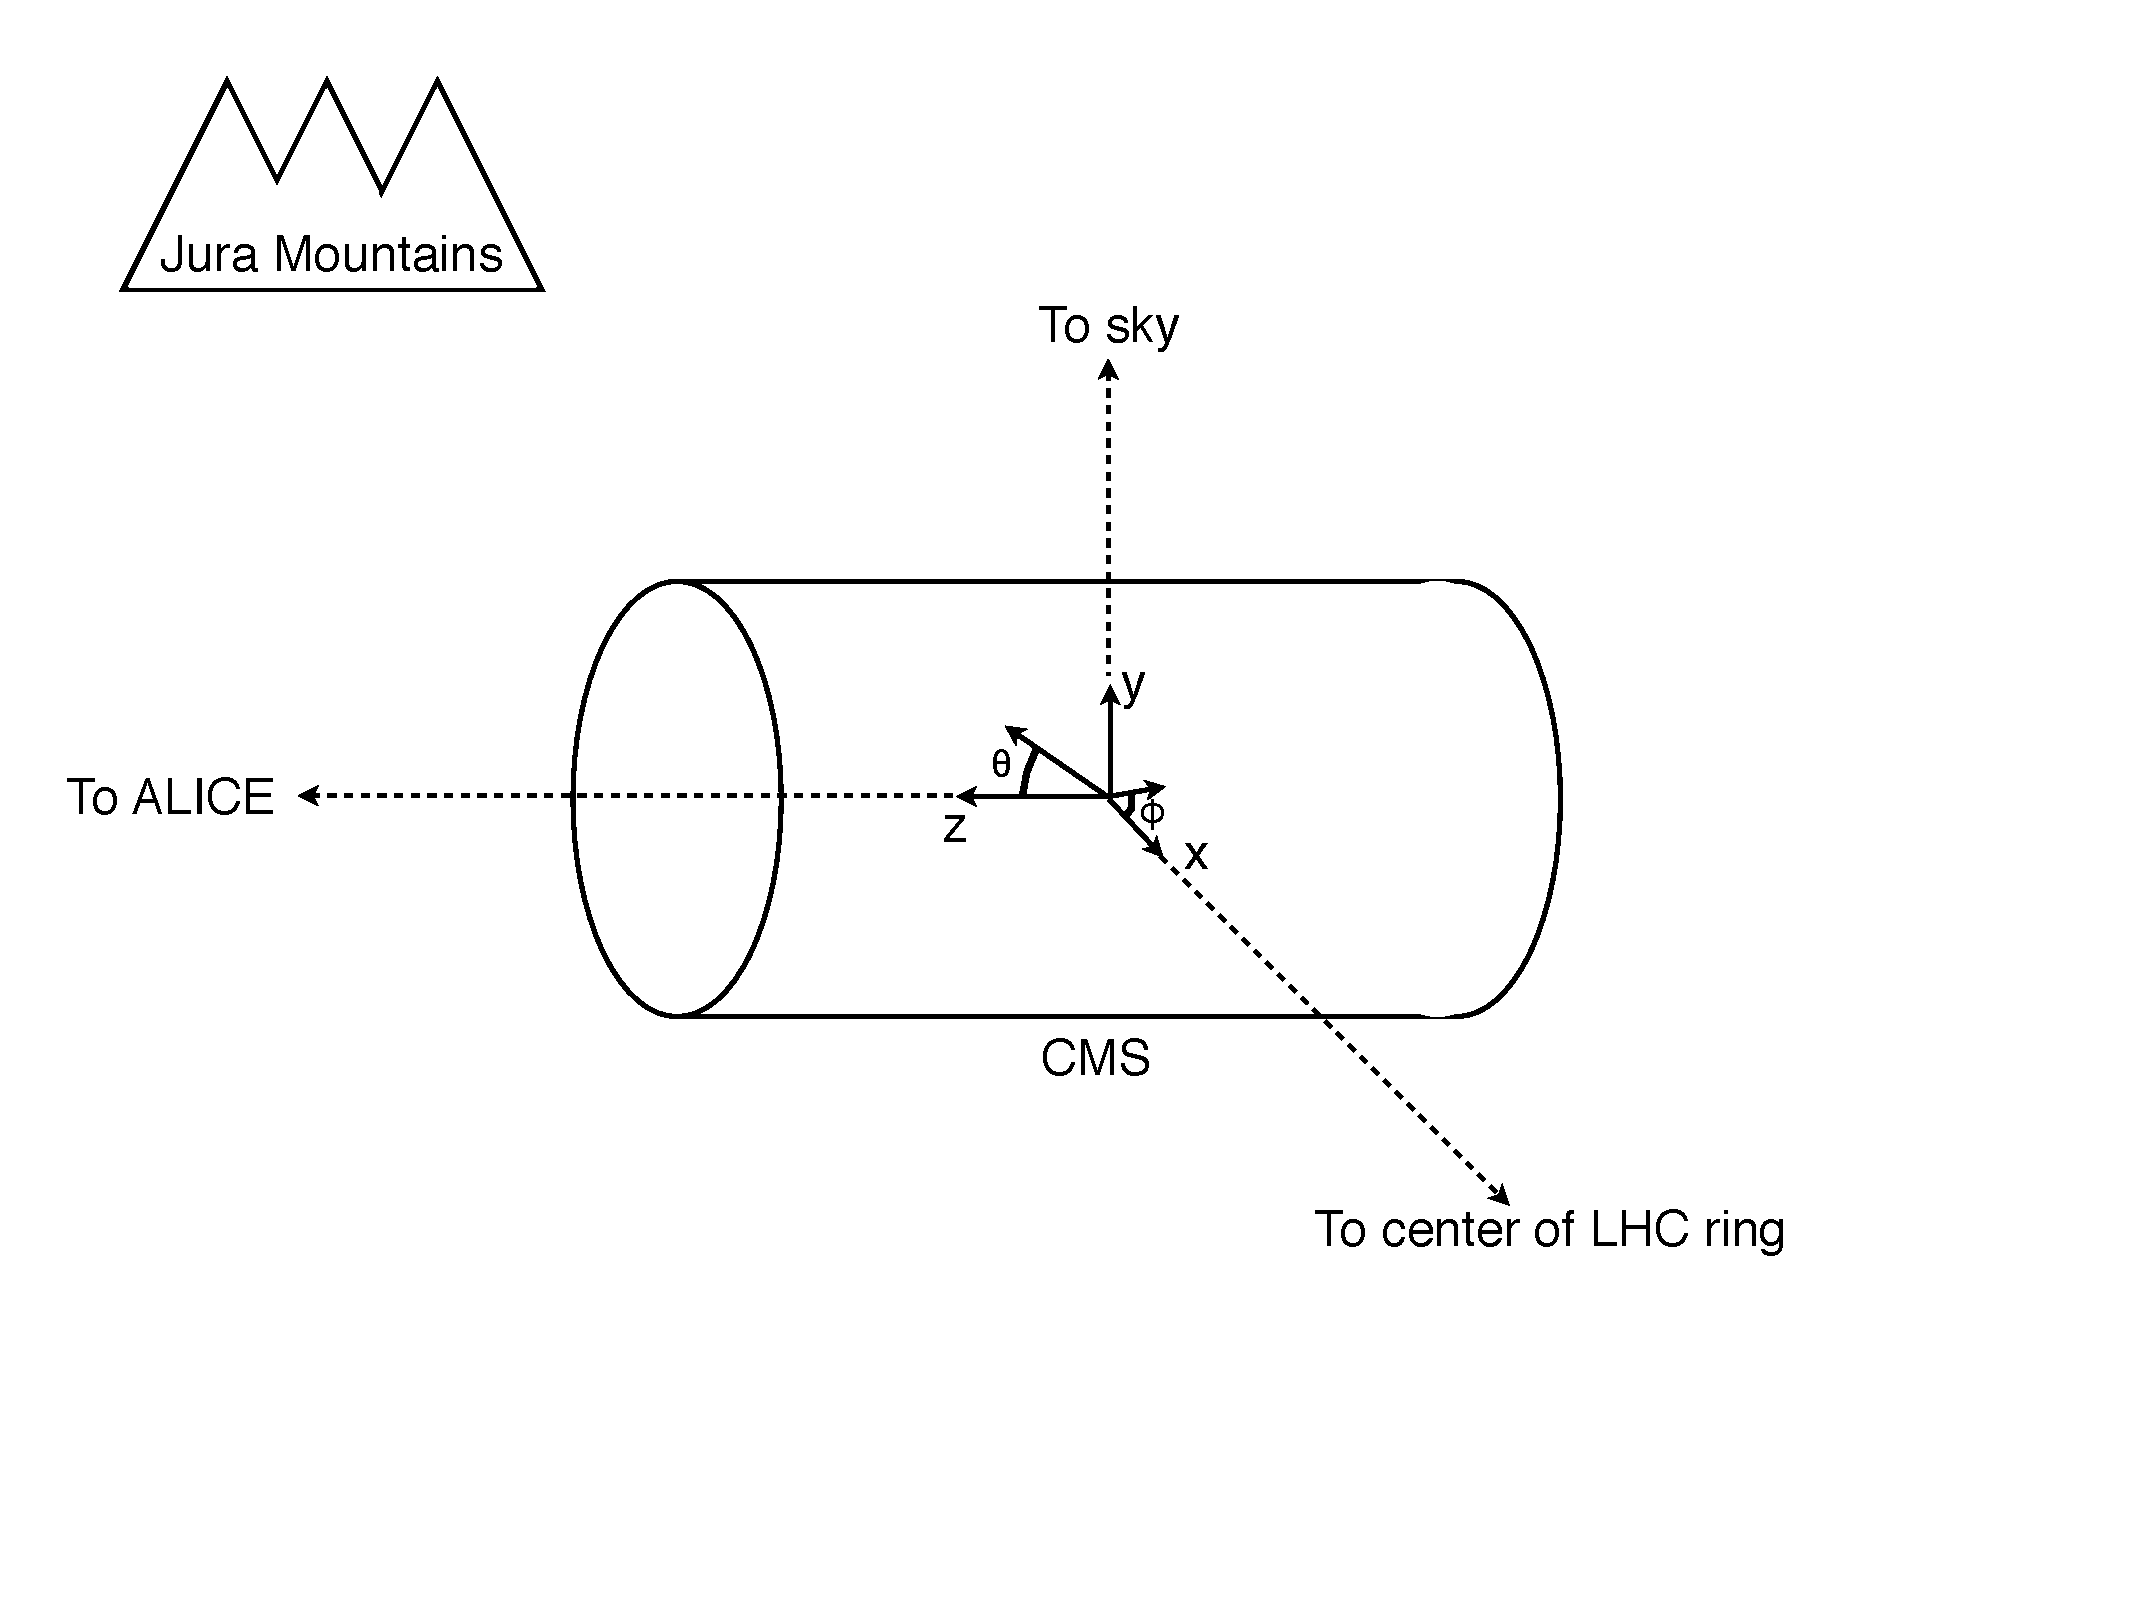
\includegraphics[scale=0.5]{CMS_coordinate_system}
	\caption{CMS coordinate system.}
	\label{fig:CMS_coordinate_system}
\end{figure}

The CMS sub-detectors are arranged in concentric cylindrical layers, plus ``endcaps," around the beam line, as shown in Figure~\ref{fig:CMS_cutaway}.  Closest to the beam line are three layers of silicon pixel detectors, with the innermost at radius 4.4 cm and outermost at radius 10.2 cm \cite{1748-0221-3-08-S08004}.  Including the pixel endcaps, the total pixel coverage extends to $\eta$ = 2.5 \cite{1748-0221-3-08-S08004}.  The pixel detector plays in important role in determining the proton-proton interaction position (\textit{beam spot}) and the impact parameters of charged particle trajectories, and is critical for the measurement of decay positions some distance from the beam spot (\textit{displaced vertices}), such as those due to the showering and hadronization of a $b$ quark.

\begin{figure}
	\centering
	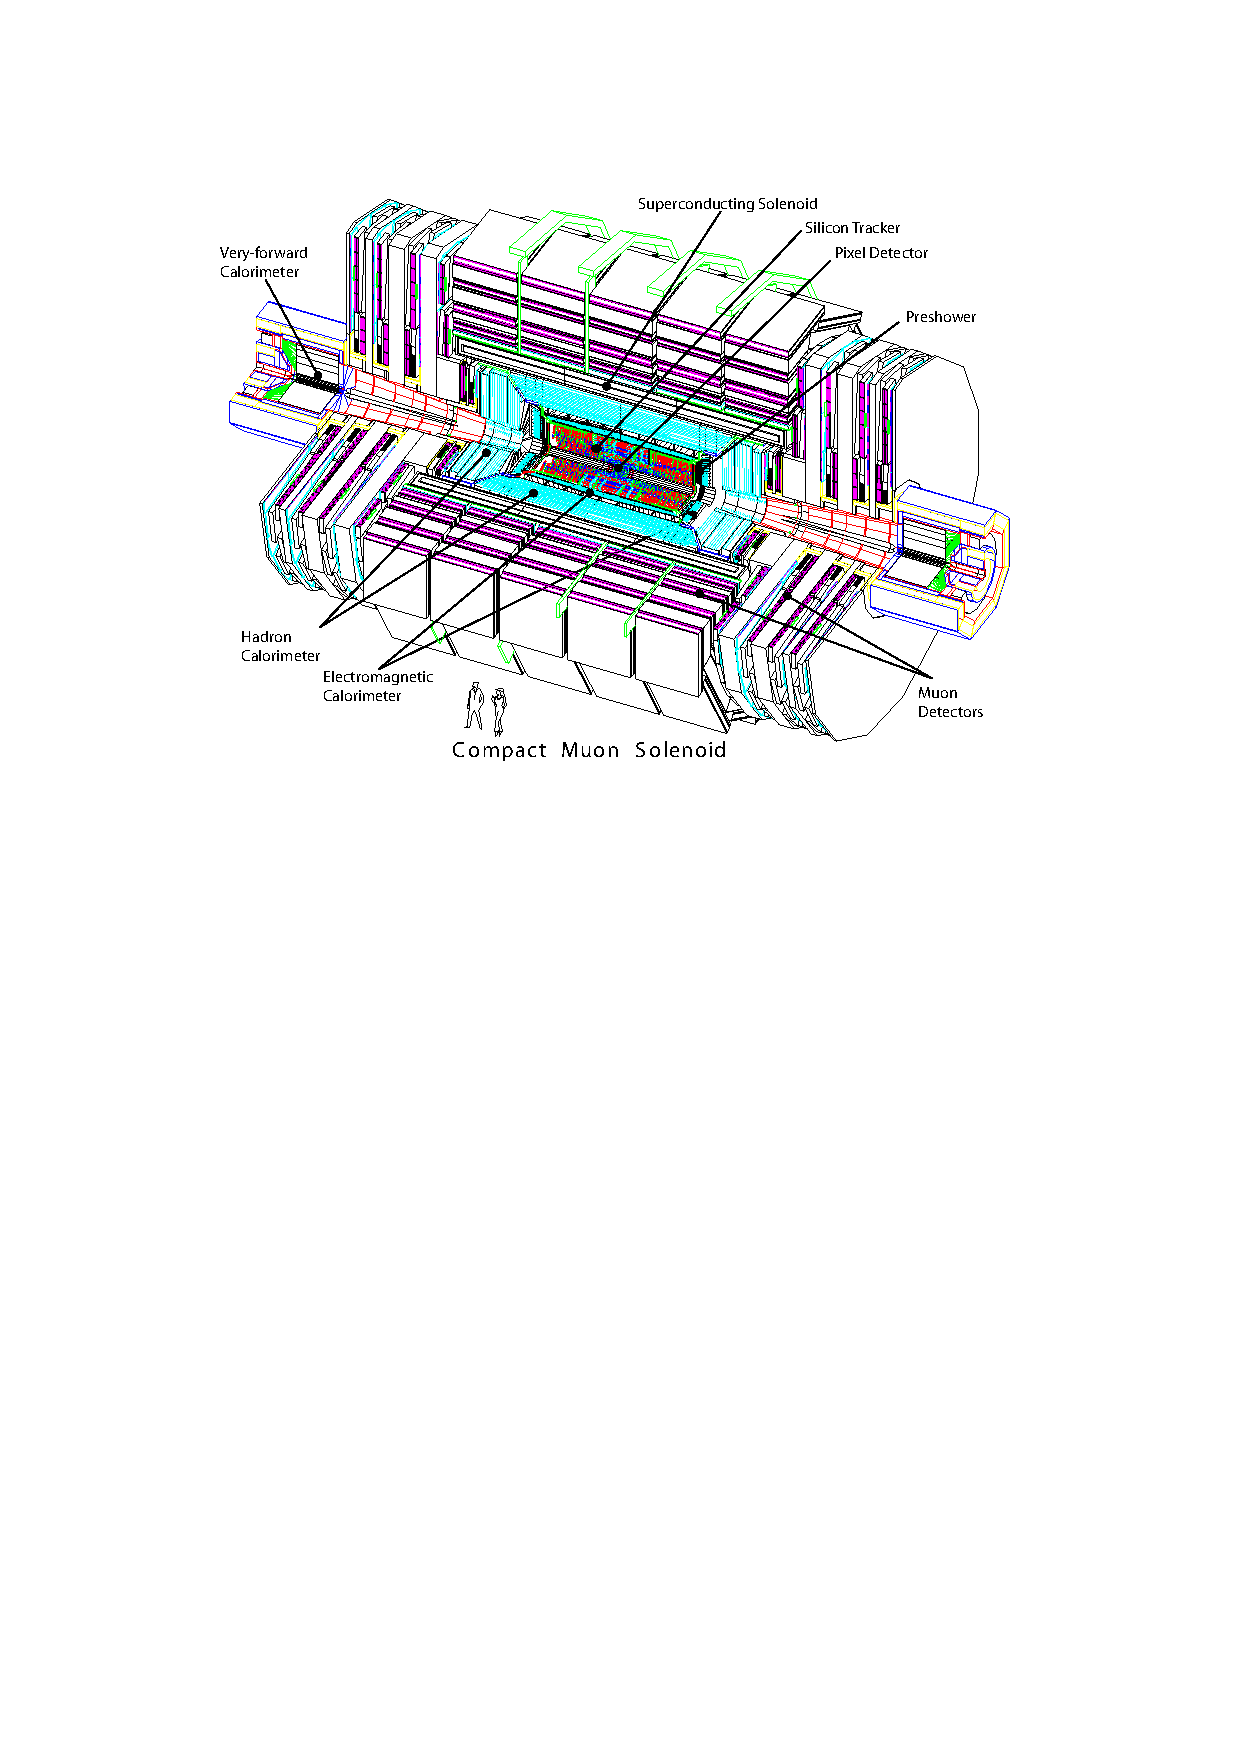
\includegraphics[scale=1.0]{CMS_cutaway}
	\caption{Cutaway view of CMS.  Reprinted from Fig. 1.1 of ref. \cite{1748-0221-3-08-S08004}.}
	\label{fig:CMS_cutaway}
\end{figure}

The 10 next layers of CMS are comprised of silicon microstrip detectors, with the outermost layer at a radius of 1.3 m from the beam line \cite{1748-0221-3-08-S08004}.  As for the pixel detectors, the silicon strip endcaps extecnd tracking coverage to $\eta$ = 2.5.  The silicon microstrip layers are the workhorse of the CMS tracking system, and provide excellent charged particle momentum resolution and track finding efficiency.

Outside the tracking detectors are the calorimeters, starting with the single-layer lead tungstate crystal electromagnetic calorimeter at a radius of 1.3 m from the beam line (location of crystal front faces) \cite{1748-0221-3-08-S08004}.  Each crystal is 23 cm long, corresponding to 25.8 radiation lengths ($\mbox{X}_{0}$)  \cite{1748-0221-3-08-S08004}.  The crystal dimensions are such that most of one electromagnetic shower, and no more, can be contained in a single crystal, leading to excellent energy resolution for photons and electrons.  The electromagnetic calorimeter radial and endcap layers cover a pseudorapidity range up to 3.0.  A lead/silicon sampling calorimeter sits in front of the crystal endcaps to provide better rejection of neutral pions.

The last layer of calorimetry inside the solenoid is the brass/scintillator sampling hadronic calorimeter, which has a radial extent from 1.77-2.95 m \cite{1748-0221-3-08-S08004}.  The hadronic barrel and endcap calorimeters cover up to $|\eta|$ = 3.0, while the iron/quartz-fiber forward hadronic calorimeter covers the region $3.0 \leq |\eta| \leq 5.2$. \footnote{The Centauro and Strange Object Research (CASTOR) and Zero Degree Calorimeter (ZDC) detectors provide additional calorimetry beyond $|\eta| = 5.2$.  However, they are mainly used in the heavy ion and diffractive physics programs of CMS, and play no role in the detection of heavy SUSY particles.  Therefore, they will not be discussed here.}  There is one more layer of hadronic calorimetry outside the solenoid in $|\eta| < 1.3$ which, together with the layers inside the solenoid, provides approximately 12 hadronic interaction lengths of instrumented absorber.  Because of its large $|\eta|$ coverage and depth, the hadronic calorimeter provides good missing transverse energy resolution and accurate measurements of high energy jets.

The iron return yoke of the solenoidal magnetic field is interleaved with muon detectors from 4.1-7.4 m in $r$ and 6.6-10.6 m in $z$, providing muon detection up to $|\eta| = 2.4$ \cite{1748-0221-3-08-S08004}.  In the barrel region of $|\eta| < 1.2$, drift tubes are used to read out the muon tracks, while in the endcaps cathode strip chambers are used.  Due to their speed, resistive plate chambers are used throughout the muon system to provide an independent trigger and timing measurement.  Combining the tracker and muon system hits, the momenta and charge of muons up to $p_{T} = 1$ TeV can be precisely reconstructed.

A longitudinal quarter cross-sectional view of CMS is shown in Figure~\ref{fig:CMS_longitudinal_xsec}.  The remainder of this chapter is devoted to explaining the CMS subdetectors and readout systems.  Section~\ref{sec:The Detectors and Their Operating Principles} describes the subdetector technologies and performance benchmarks, while Section~\ref{sec:Triggering, Data Acquisition, and Data Transfer} details the CMS trigger and data acquisition systems and framework for promptly reconstructing and transferring data worldwide.  For a thorough description of CMS, see ref. \cite{1748-0221-3-08-S08004}.  Unless otherwise noted, all information in this chapter comes from ref. \cite{1748-0221-3-08-S08004}.

\begin{figure}
	\centering
	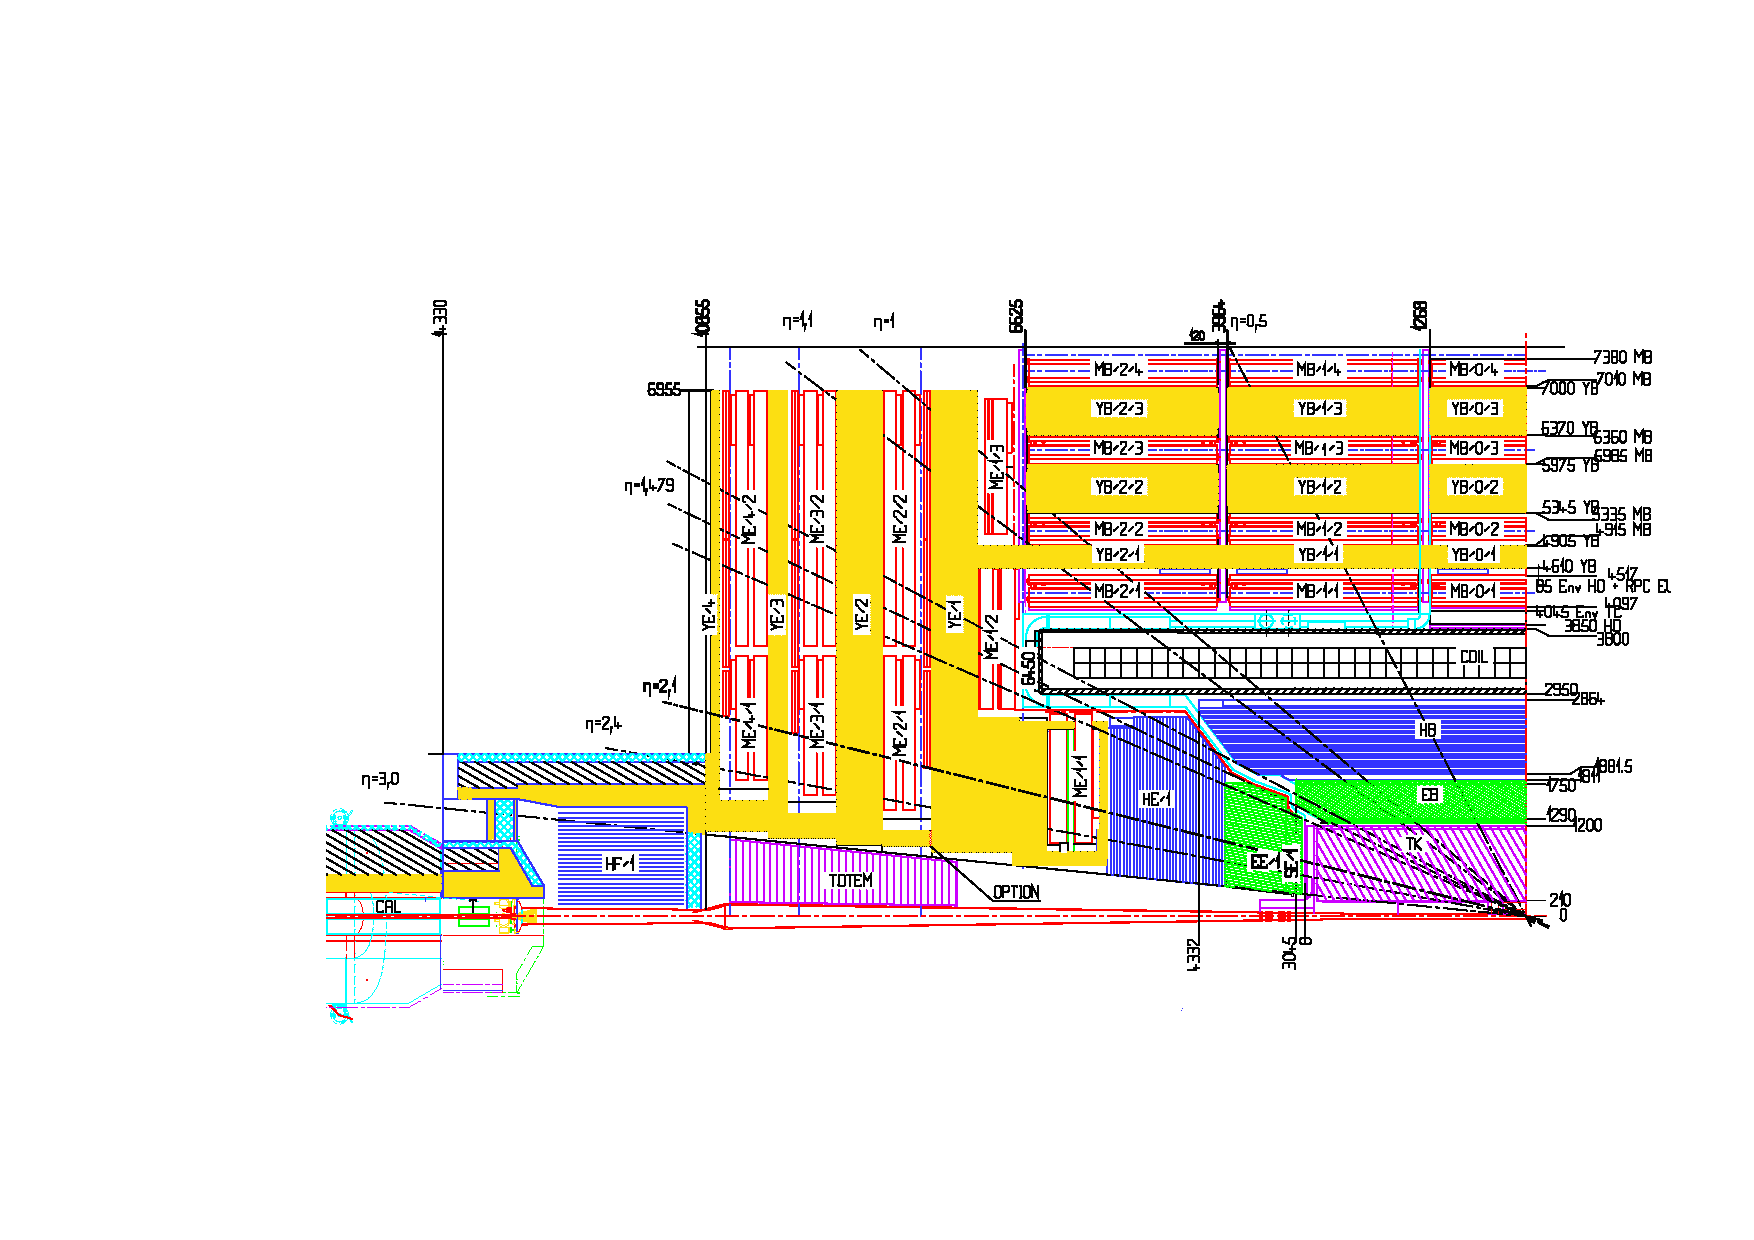
\includegraphics[scale=0.5]{CMS_longitudinal_xsec}
	\caption{Longitudinal quarter cross-sectional view of CMS.  The nominal interaction point is at the lower right-hand corner of the drawing.  The tracker is shown in purple diagonal hashing, the electromagnetic calorimeter in green, the hadronic calorimeter in blue, and the muon stations in red.  The solenoid is shown in black and white and labeled \texttt{COIL}, and the magnet return yoke is shown in yellow.  Radial and longitudinal distances are measured in millimeters.  Reprinted from Fig. CP 1 of ref. \cite{Bayatian:922757}.}
	\label{fig:CMS_longitudinal_xsec}
\end{figure}

\section{The Detectors and Their Operating Principles}
\label{sec:The Detectors and Their Operating Principles}

\subsection{Tracking System}
\label{sec:Tracking System}

Given the LHC design instantaneous luminosity, efficient reconstruction of charged particle tracks from transverse momenta of 1 GeV up to 1 TeV can only be achieved with a low occupancy tracker.  For $r < 10$ cm, the hit rate density is highest, leading to the choice of $100\mbox{ }\mu\mbox{m} \times 150\mbox{ }\mu\mbox{m}$ silicon pixel sensors for hit detection.  For $20\mbox{ cm }< r < 110\mbox{ cm}$, the lower hit rate allows the use of silicon strips, with length along $z$ of order centimeters and length along the $r\cdot\phi$ curve of order hundreds of microns.  This design leads to a pixel hit occupancy of $\sim10^{-4}$/pixel/BX and a strip hit occupancy of $\sim10^{-2}$/pixel/BX, where BX refers to 1 LHC bunch crossing.

As radiation dose from hadrons accumulates over the lifetime of the tracker, silicon leakage current through the semiconductor junctions increases, heating up the sensors.  Since the leakage current itself depends on temperature, this can lead to \textit{thermal runaway} that damages the detector.  To avoid this, the tracker must be cooled to approximately $-10^{\circ}$C.  Operating at this temperature, the signal:noise ratio in the silicon sensors is 10:1, and should remain at that level over the 10-year lifetime of the tracker.

At its thickest ($|\eta|\sim1.5$), the tracker depth (including services) is $\sim1.8X_{0}$, and the depth falls off to $\sim1X_{0}$ in thinner areas.  Unfortunately, the large mass of the tracker degrades somewhat the performance of the electromagnetic calorimeter behind it, as $\sim50$\% of photons will convert to $e^{+}e^{-}$ pairs in the tracker.

\subsubsection{Pixel Detector}
\label{sec:Pixel Detector}

A longitudinal quarter view of the three barrel pixel (BPix) layers and two forward pixel (FPix) disks is shown in Figure~\ref{fig:pixel_longitudinal_quarter_view}.  There are 768 BPix modules in total.  Each BPix layer is divided into 32 $\phi$-wedges, with eight modules per wedge arranged end-to-end in $z$.  The $\phi$-wedges operate nearly independently in terms of clock and readout.  Each FPix disk consists of 24 $\phi$-wedges, with pie-shaped modules attached to the front and back of the disk, for a total of 192 modules.  The front- and back-side modules of the FPix disks are constructed of different sized \textit{plaquettes}, or multi-pixel sensor chips, such that the gaps in the front-side module are covered by plaquette area in the back-side module and vice versa.  An illustration of the BPix and FPix mechanical layouts is given in Figure~\ref{fig:pixel_mechanics}.

\begin{figure}
	\centering
	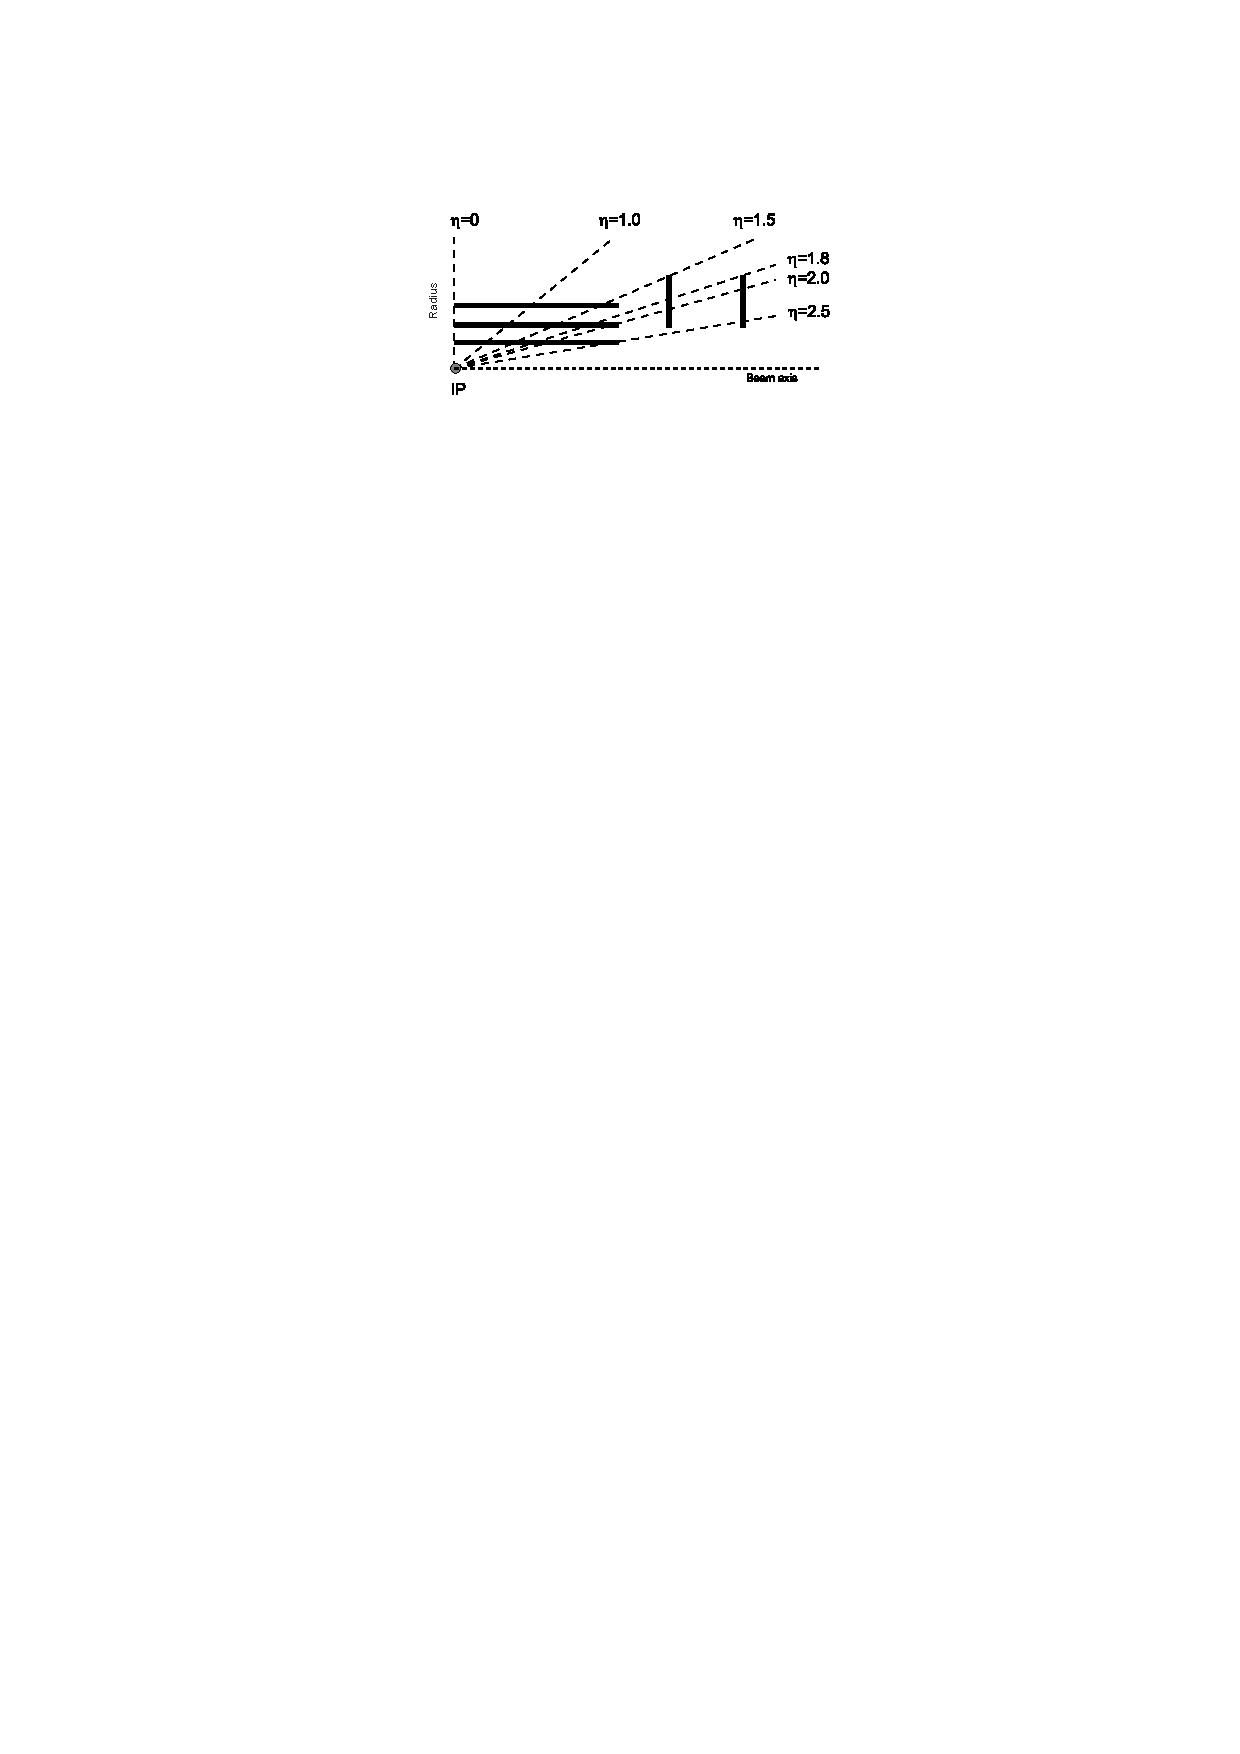
\includegraphics[scale=1.0]{pixel_longitudinal_quarter_view}
	\caption{Longitudinal quarter view of the pixel detector.  Reprinted from Fig. 3.6 of ref. \cite{1748-0221-3-08-S08004}.}
	\label{fig:pixel_longitudinal_quarter_view}
\end{figure}

\begin{figure}
	\centering
 	\subfloat[Cutaway view of the barrel pixel layers, showing the three layers and the eight end-to-end modules along $z$.  Reprinted from Fig. 3.11 of ref. \cite{1748-0221-3-08-S08004}.]{\label{fig:BPix_mechanics}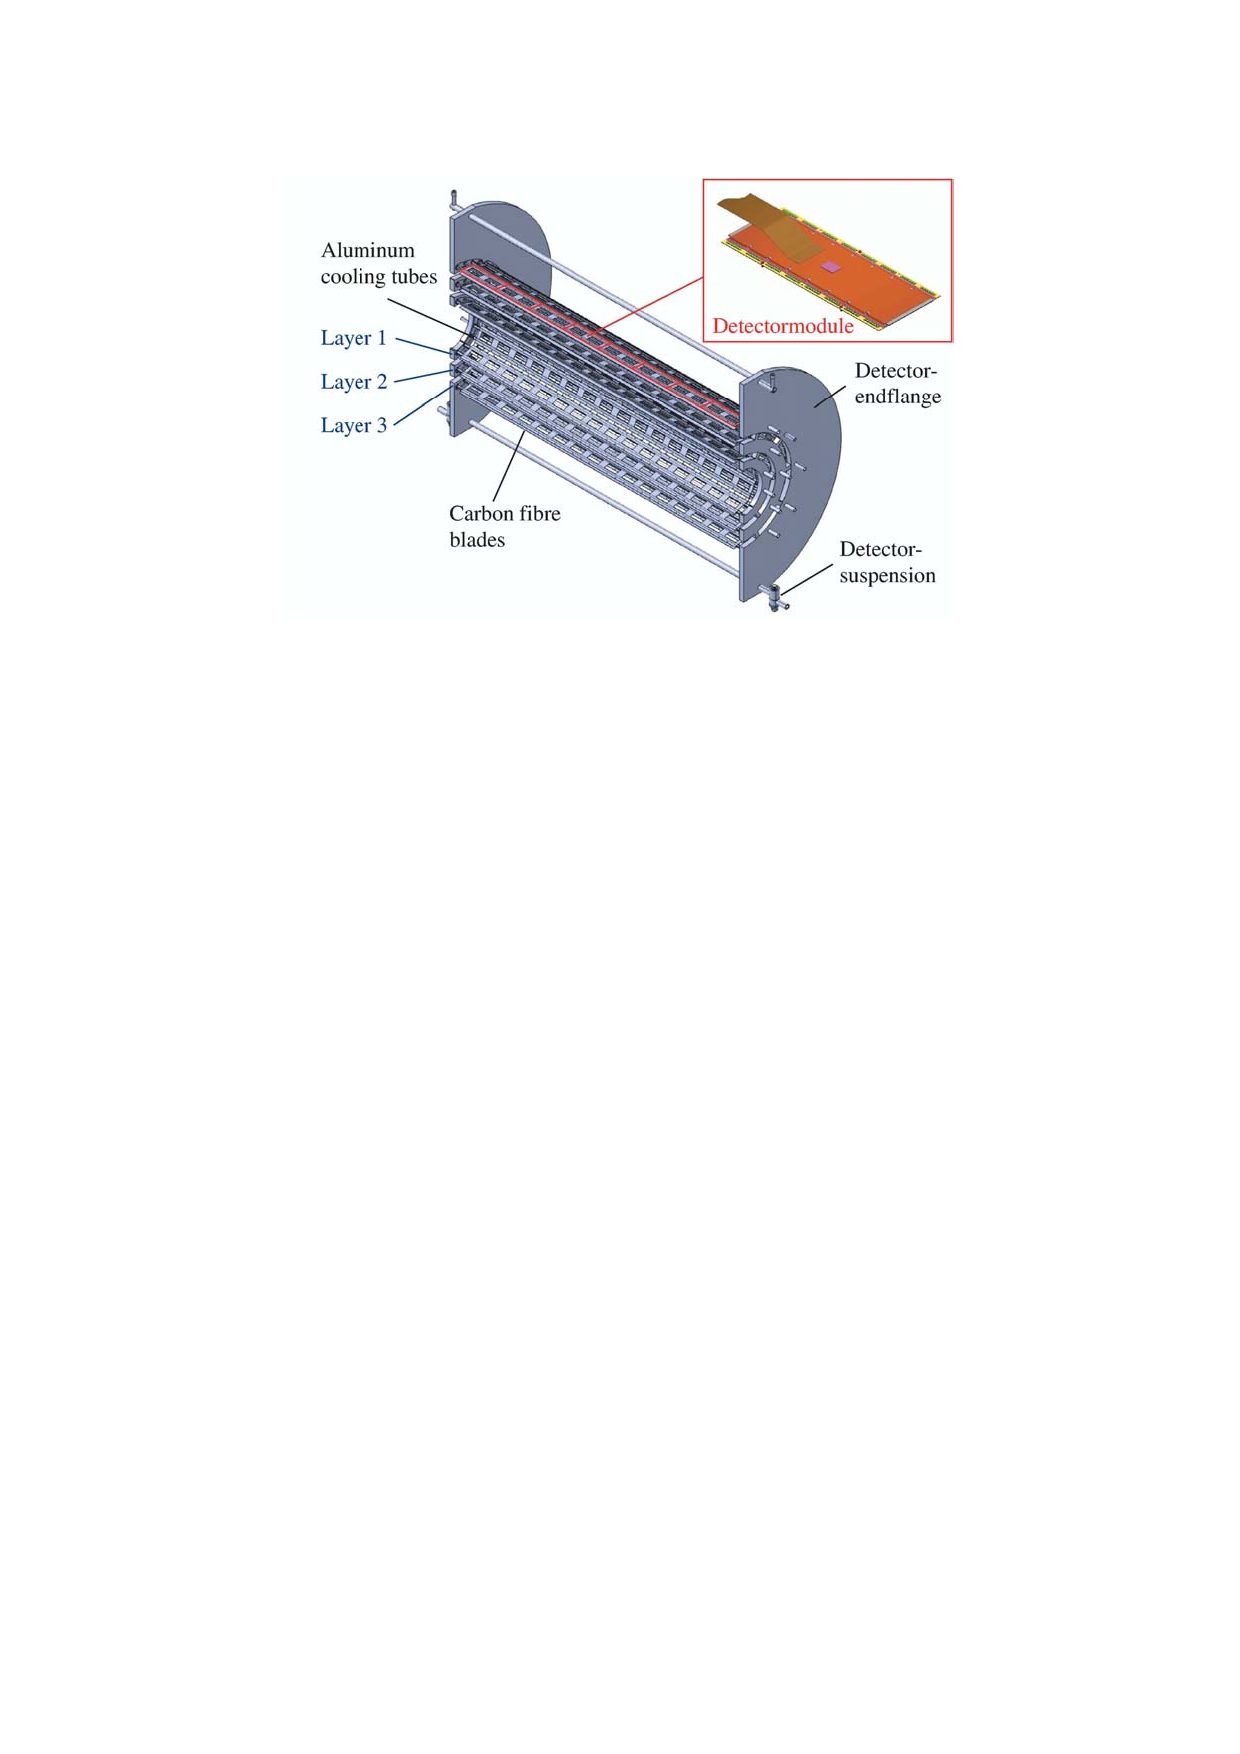
\includegraphics[scale=0.6]{BPix_mechanics}}
	\hspace{1cm}
	\subfloat[Half-disk of the foward pixel detector, showing the 12 pie-shaped module mounts.  Reprinted from Fig. 3.15 of ref. \cite{1748-0221-3-08-S08004}.]{\label{fig:FPix_mechanics}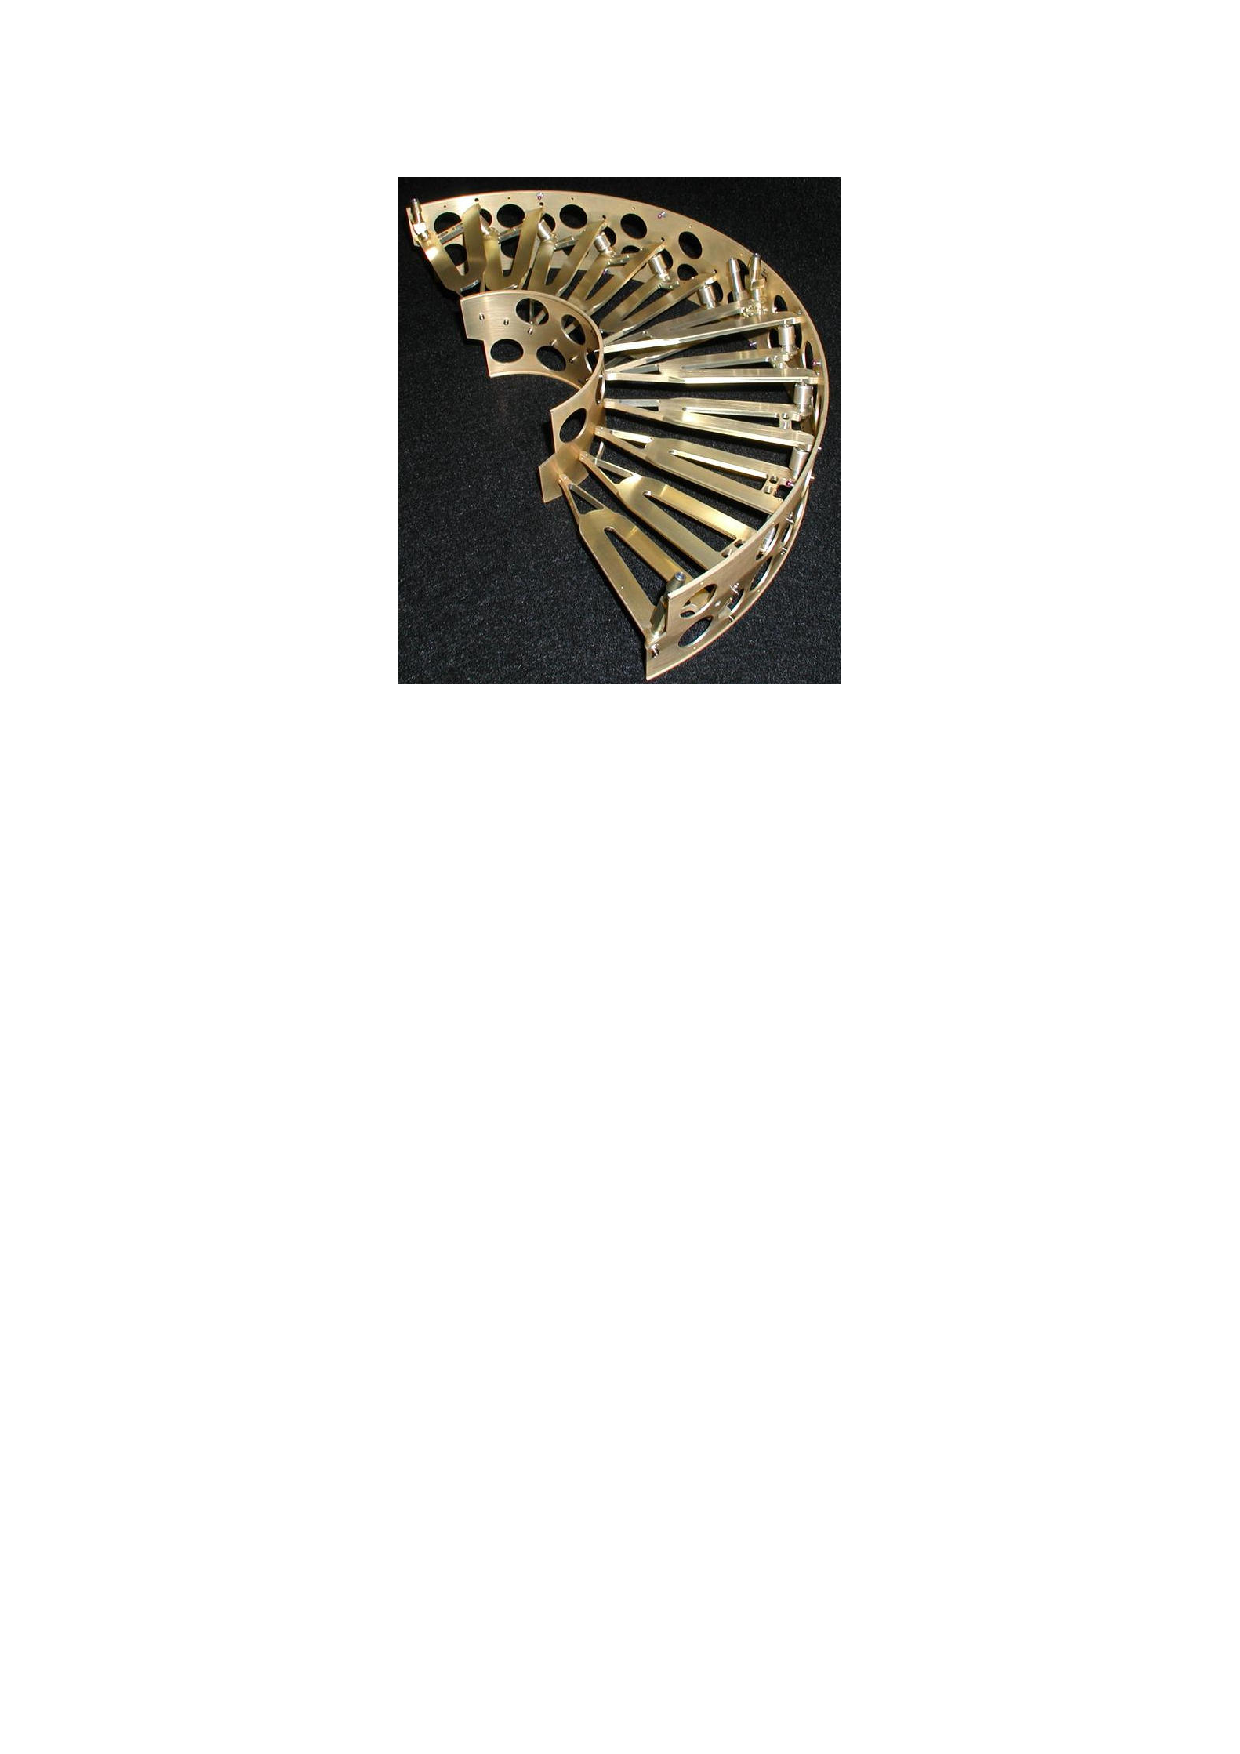
\includegraphics[scale=0.6]{FPix_mechanics}}
	\caption{BPix and FPix mechanical structures.}
	\label{fig:pixel_mechanics}
\end{figure}

Since the electric field in the depletion region of the BPix sensors is perpendicular (i.e. pointing along $r$) to the magnetic field of CMS (i.e. pointing along $z$), the charge carriers in the silicon experience a Lorentz drift along $\phi$.  The multi-pixel sensor pitch is such that this causes the charge from one particle hit to be shared among multiple pixels.  Particle hits are reconstructed reading out the analog pixel signal and interpolating between signals in multiple pixels.  This method achieves a 15-20 $\mu\mbox{m}$ spatial resolution, which is comparable to the sensor pitch.  To induce this effect in FPix, the sensor wedges are tilted by the approximate BPix Lorentz angle of $20^{\circ}$ \cite{Ivova} with respect to the $y$-axis.

Each multi-pixel sensor consists of an array of $52\times80$ n-type pixels implanted onto an n-type substrate with 320 $\mu\mbox{m}$ thickness.  The other face of the substrate is covered with a thin layer of p-type semiconductor.  Except for the outer edges, which are held at ground potential to prevent sparking between the sensor edges and the connected readout chip \cite{Bolla2001182}, the p-side is reverse biased at 150 V (BPix) or 300 V (FPix).  The pixels are held at ground potential.  A particle entering through the p-side will cause a burst of current to flow across the p-n junction.  The charge will be collected by the pixels, which are bump-bonded to the readout.  The BPix and FPix sensors employ slightly different technologies for electrically isolating the individual pixels, but both rely on the idea of surrounding the pixels with a p-type material to provide a p-n junction that acts as a barrier to current flow.

Each $52\times80$ pixel sensor is bump bonded to a readout chip (ROC).  The ROCs provide zero suppression and amplify,  buffer, and communicate the signals from the sensors.  A single token bit manager (TBM) controls $\sim16$ ROCs in the barrel or $\sim24$ ROCs in the endcaps.  Its purpose is to distribute the clock and trigger to the ROCs (the latter initiates a transmission of the signal further upstream to be assembled into the full event readout of CMS).  The clock and trigger are supplied by the pixel front end controller (pFEC), which interfaces to the central clock and data acquisition systems.  Analog signals that are collected from the pixel front ends are digitized by the pixel front end digitizer (pxFED).  A diagram of the readout system is shown in Figure~\ref{fig:pixel_readout}.

\begin{figure}
	\centering
	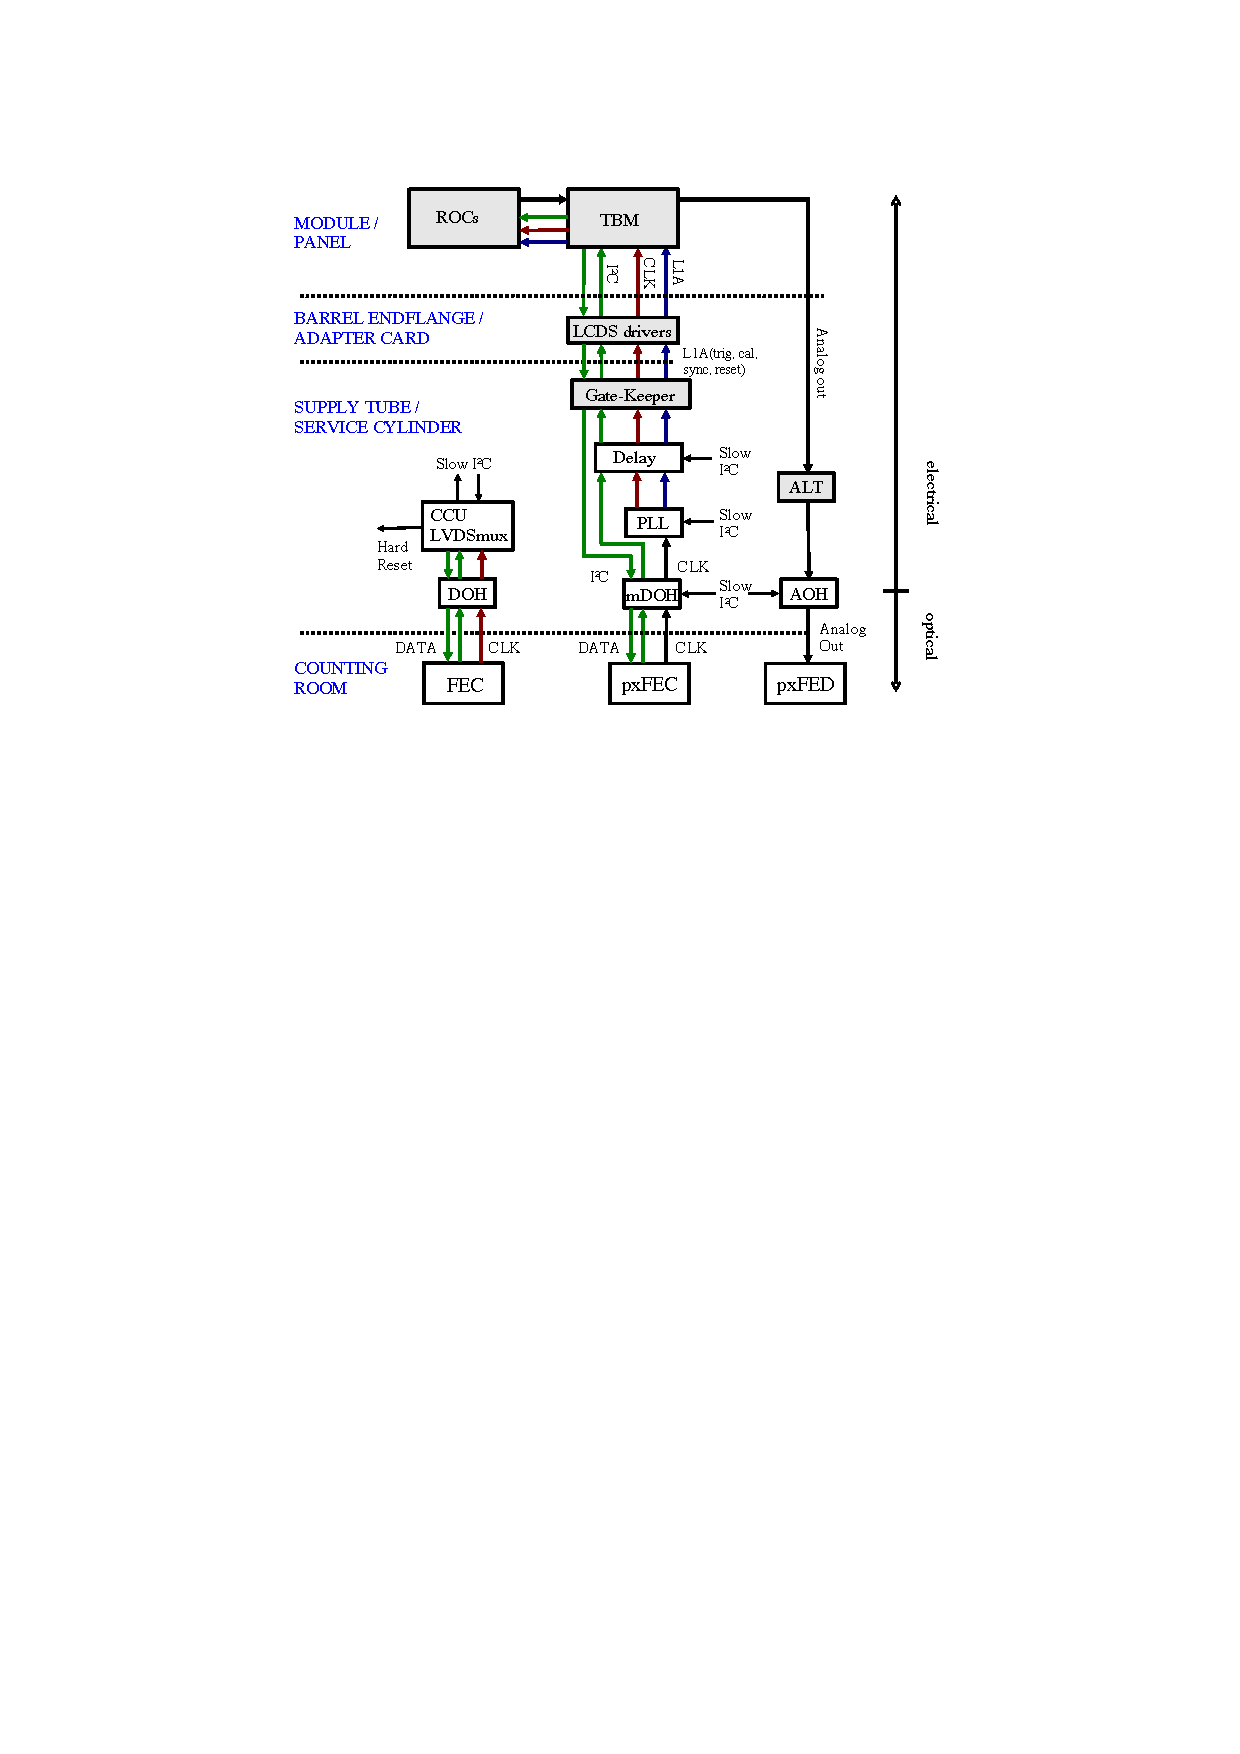
\includegraphics[scale=1.0]{pixel_readout}
	\caption{Pixel control and readout system.  Reprinted from Fig. 3.9 of ref. \cite{1748-0221-3-08-S08004}.}
	\label{fig:pixel_readout}
\end{figure}

Figure~\ref{fig:pixel_results} shows some results highlighting the performance of the pixel detector.

\begin{figure}
	\centering
 	\subfloat[BPix hit resolution in the $r\cdot\phi$ coordinate \cite{pixel_DPG_Twiki_rphi_res}.]{\label{fig:pixel_results_rphi_res}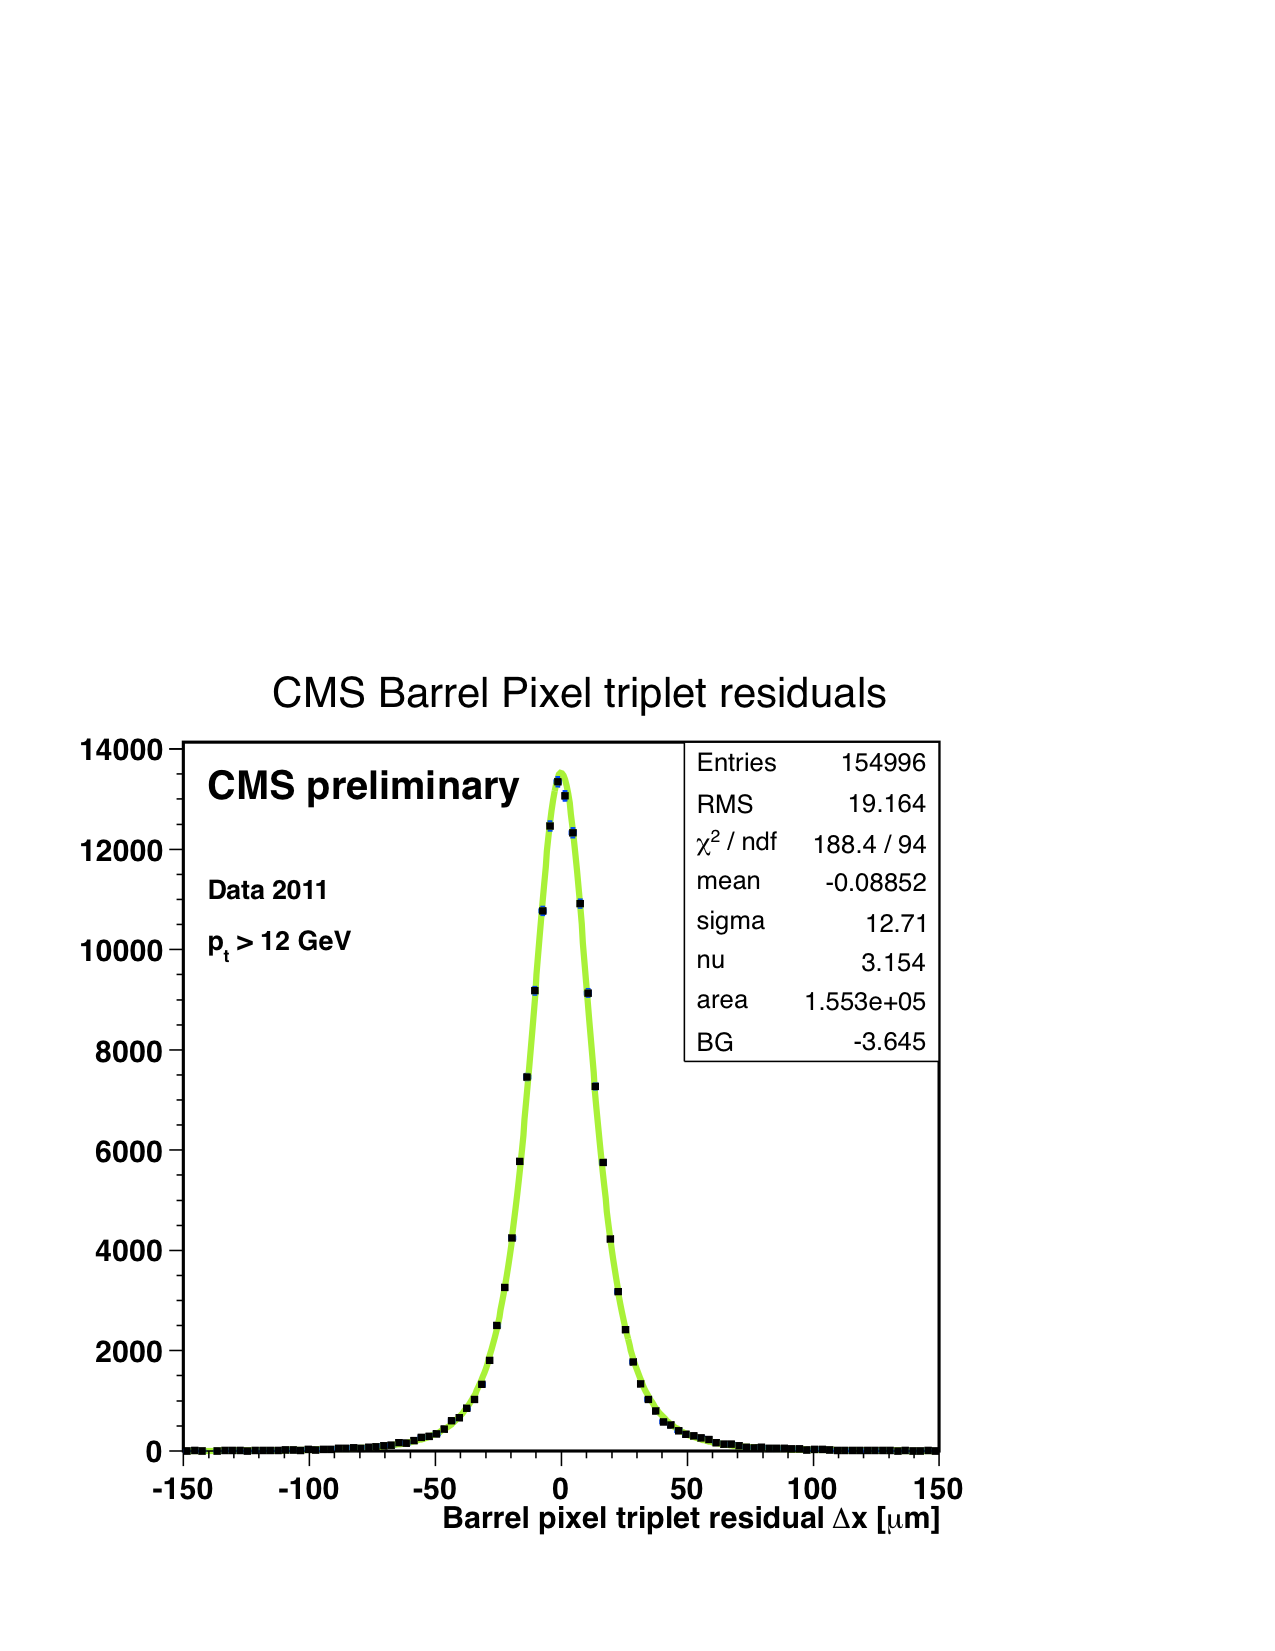
\includegraphics[scale=0.3]{pixel_results_rphi_res}}
	\hspace{1cm}
	\subfloat[BPix hit resolution in the $z$ coordinate vs. track dip angle, showing the effect of charge sharing on resolution \cite{pixel_DPG_Twiki_z_res}.]{\label{fig:pixel_results_z_res}\includegraphics[scale=0.3]{pixel_results_z_res}}
	\\
	\subfloat[Pixel reconstruction efficiency vs. bias voltage for a group of three wedges in FPix \cite{pixel_DPG_Twiki_eff}.]{\label{fig:pixel_results_eff}\includegraphics[scale=0.3]{pixel_results_eff}}
	\caption{Pixel detector performance highlights.}
	\label{fig:pixel_results}
\end{figure}

\subsubsection{Silicon Strip Tracker}
\label{sec:Silicon Strip Tracker}

The silicon strip tracker is divided into four parts: the inner barrel (TIB) and inner disks (TID), covering the radial extent $20\mbox{ cm} < r < 55\mbox{ cm}$ and $z$ extent $80\mbox{ cm} < |z| < 90\mbox{ cm}$; and the outer barrel (TOB) and endcap (TEC), covering the radial extent $61\mbox{ cm} < r < 108\mbox{ cm}$ and $z$ extent $124\mbox{ cm} < |z| < 282\mbox{ cm}$.  A number of the tracker layers and endcaps hold double-sided strip modules (shown as double lines in Figure~\ref{fig:strip_longitudinal_xsec}), with the rear module tilted at an angle of 100 mrad with respect to the front module, to provide a measurement in two coordinates.  There are a total of 15,148 modules in the tracker, arranged as shown in the longitudinal cross-sectional view of Fig.~\ref{fig:strip_longitudinal_xsec}.  For the TIB and TOB, the modules are arranged in straight rows end-to-end along $z$, with repeating rows covering the full $2\pi$ extent in $\phi$.  In each of the TID disks, the modules are arranged into three concentric circular rings of increasing $r$.  In the TEC, the modules are affixed to $\phi$-wedges called $\textit{petals}$.   One side of the TEC and its petal structure is shown in Figure~\ref{fig:tracker_TEC}.

\begin{figure}
	\centering
	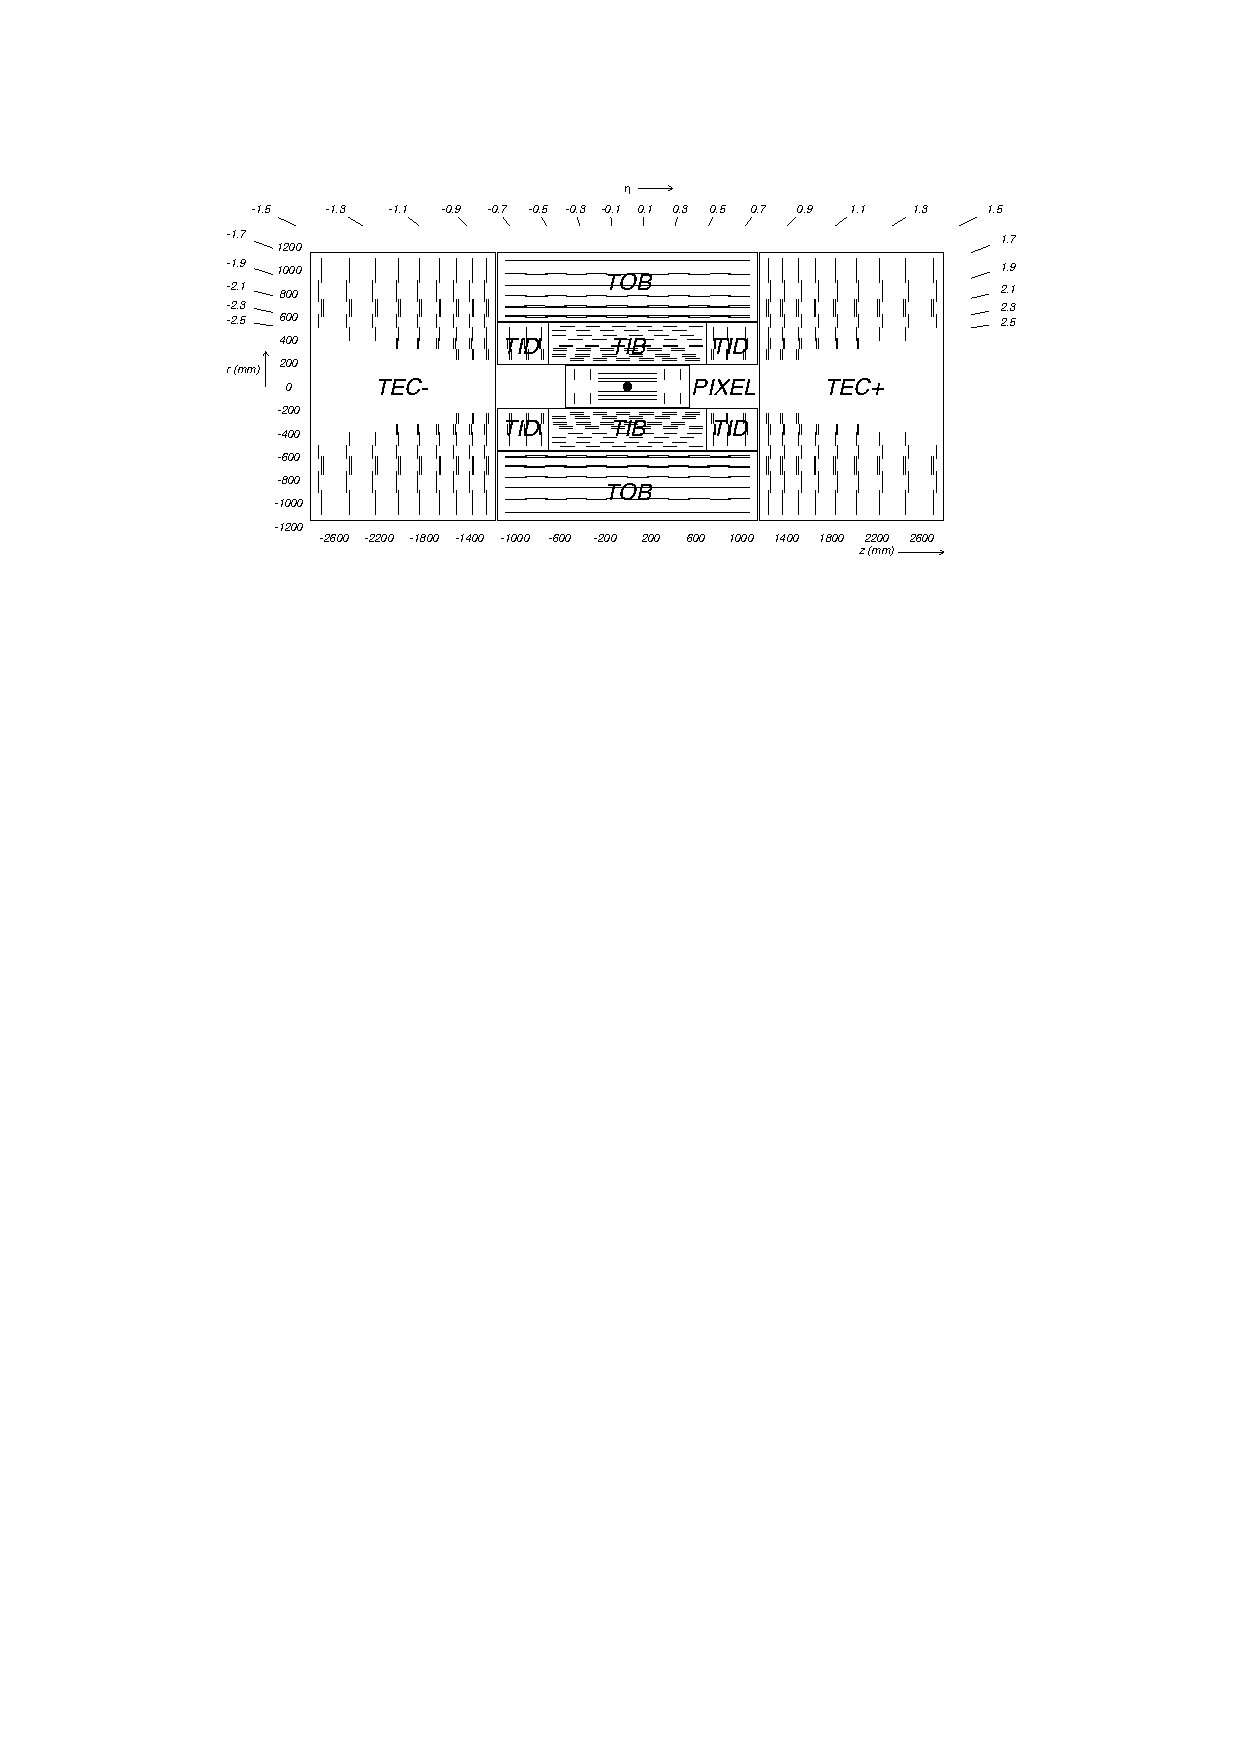
\includegraphics[scale=1.0]{strip_longitudinal_xsec}
	\caption{Longitudinal cross section of the silicon strip detector.  Reprinted from Fig. 3.1 of ref. \cite{1748-0221-3-08-S08004}.}
	\label{fig:strip_longitudinal_xsec}
\end{figure}

\begin{figure}
	\centering
	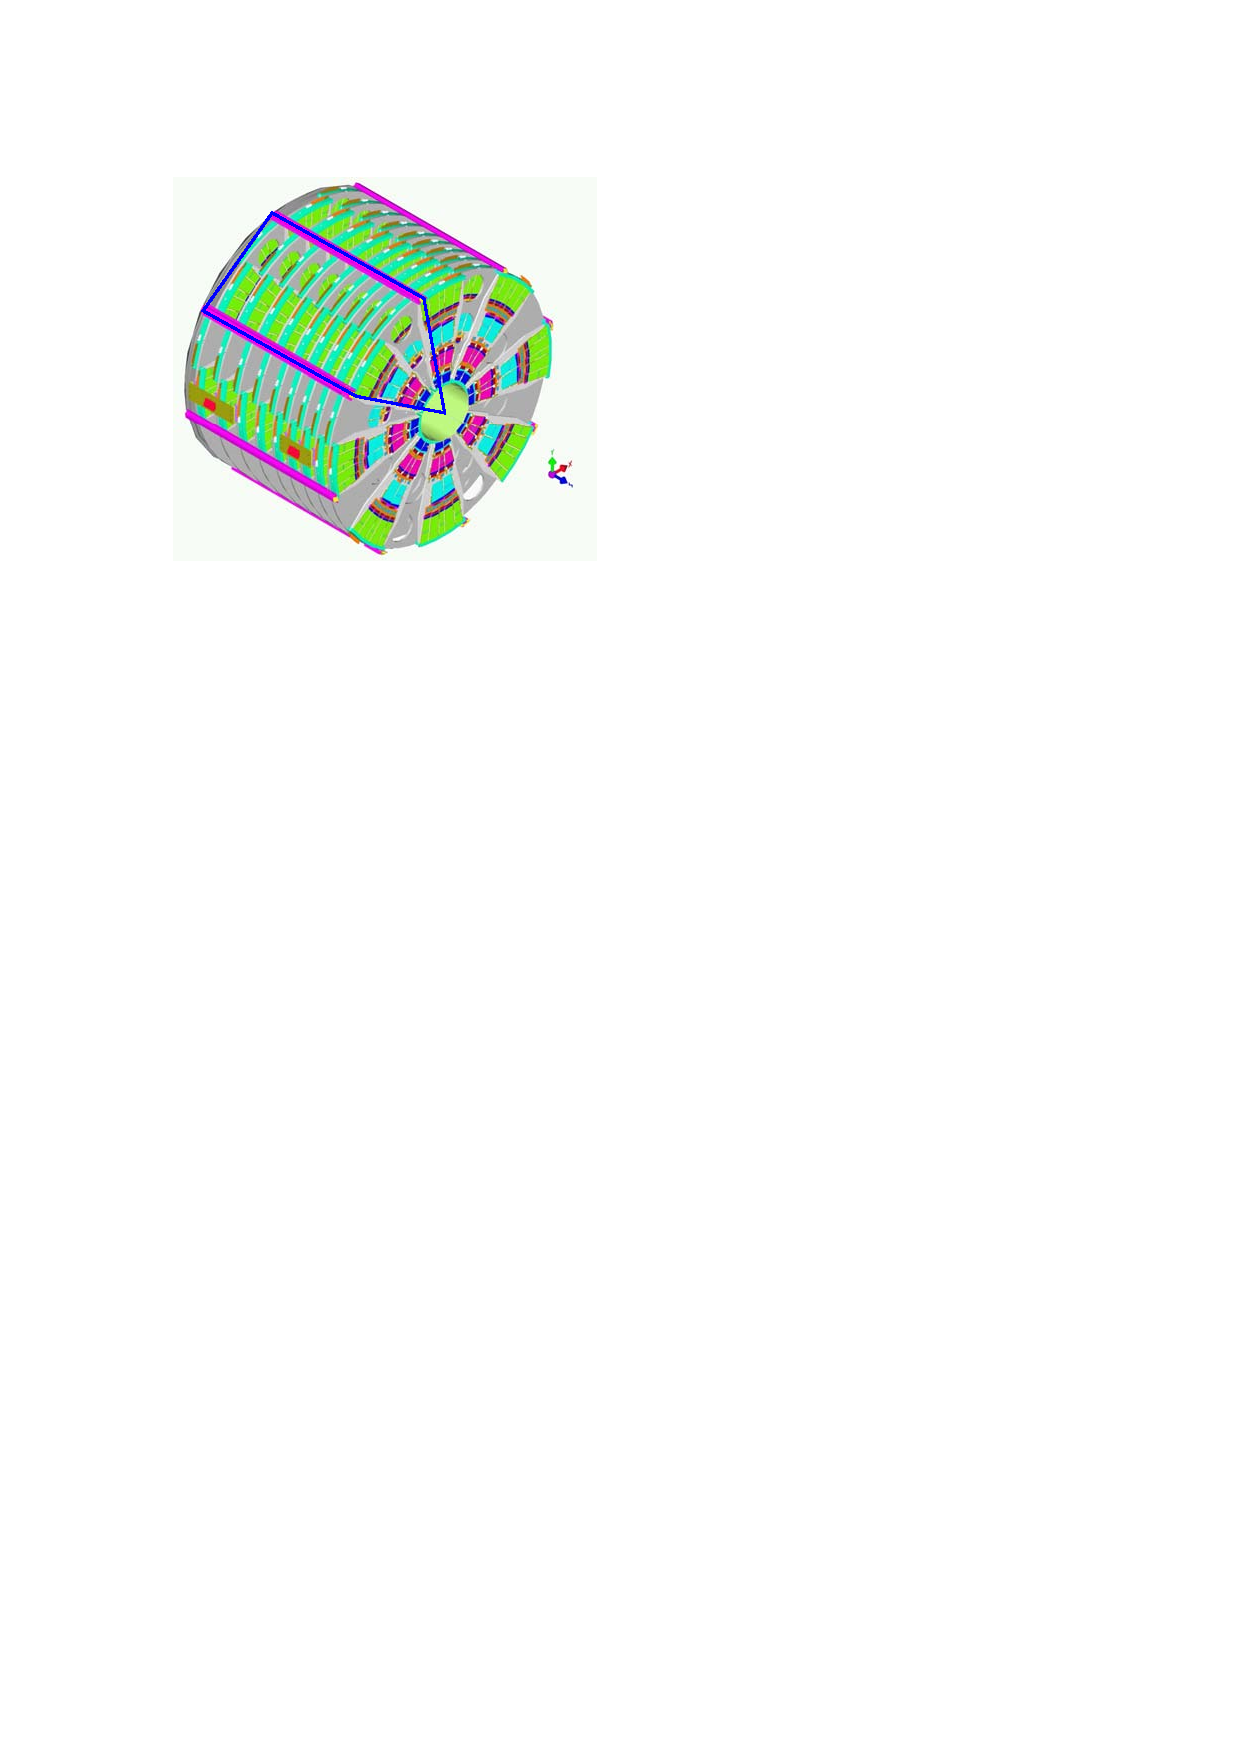
\includegraphics[scale=1.0]{tracker_TEC}
	\caption{View of one tracker endcap, with the outline of a petal shown in blue.  There are nine petals per wedge-shaped sector (one per TEC disk).  Reprinted from Fig. 3.30 of ref. \cite{1748-0221-3-08-S08004}.}
	\label{fig:tracker_TEC}
\end{figure}

Like the pixels, the strip sensors generate a signal when current flows across a p-n junction in response to interaction with a charged particle.  Whereas the pixels are n-type implants on an n-type substrate, with a solid p-type rear layer to which the high voltage is connected, the strips are p-type implants on an n-type substrate, with a solid n-type rear layer connecting to the high voltage.  The p-n junction in the strip sensors is at the strip-substrate boundary, whereas in the pixel sensors it is at the boundary between the rear layer and the substrate.  Each sensor has either 512 or 768 electrically isolated strips, with pitch varying from 80-205 $\mu\mbox{m}$ depending on location.  Strip lengths in $z$ range from $\sim10$ to $\sim25$ cm.  Thin (320 $\mu\mbox{m}$) sensors are used in the TIB, TID, and inner four rings of the TEC, while thick (500 $\mu\mbox{m}$) sensors are used in the TOB and the outer rings of the TEC.  The thicker sensors compensate for the increased strip capacitance (and hence electronics noise) of the longer strips in the outer layers/disk of the tracker such that strip signal:noise is maintained above 10 everywhere.

The strips are wire bonded to a front end readout chip called the APV25.  The APV25 amplifies and shapes the strip signals before sending the full analog pulse information to an APVMUX, which multiplexes the output of two APV25s.   Then, the electrical signal from the APVMUX is set differentially a few centimeters to an optical driver, where it is converted to an optical signal and sent to one of the 450 front end drivers (FEDs).  The FEDs convert the signal back to an electrical pulse and digitize it for use in the global event assembly.  As for the pixels, analog readout is used on detector so that hit reconstruction may benefit from charge sharing.

Clock, trigger, and control signals are sent from the front end controllers (FECs) to phase locked loop (PLL) chips on the front ends.  The FECs interface to the global clock and trigger system.  Four or six APV25s, an APVMUX, and a PLL chip all sit on a \textit{hybrid}, two which one thin or two thick sensors are also affixed.  The sensor-hybrid combination and its frame form a module.  Figure ~\ref{fig:tracker_module} shows a diagram of a module, while Figure~\ref{fig:tracker_readout} shows a block diagram of the strip readout architecture.

\begin{figure}
	\centering
	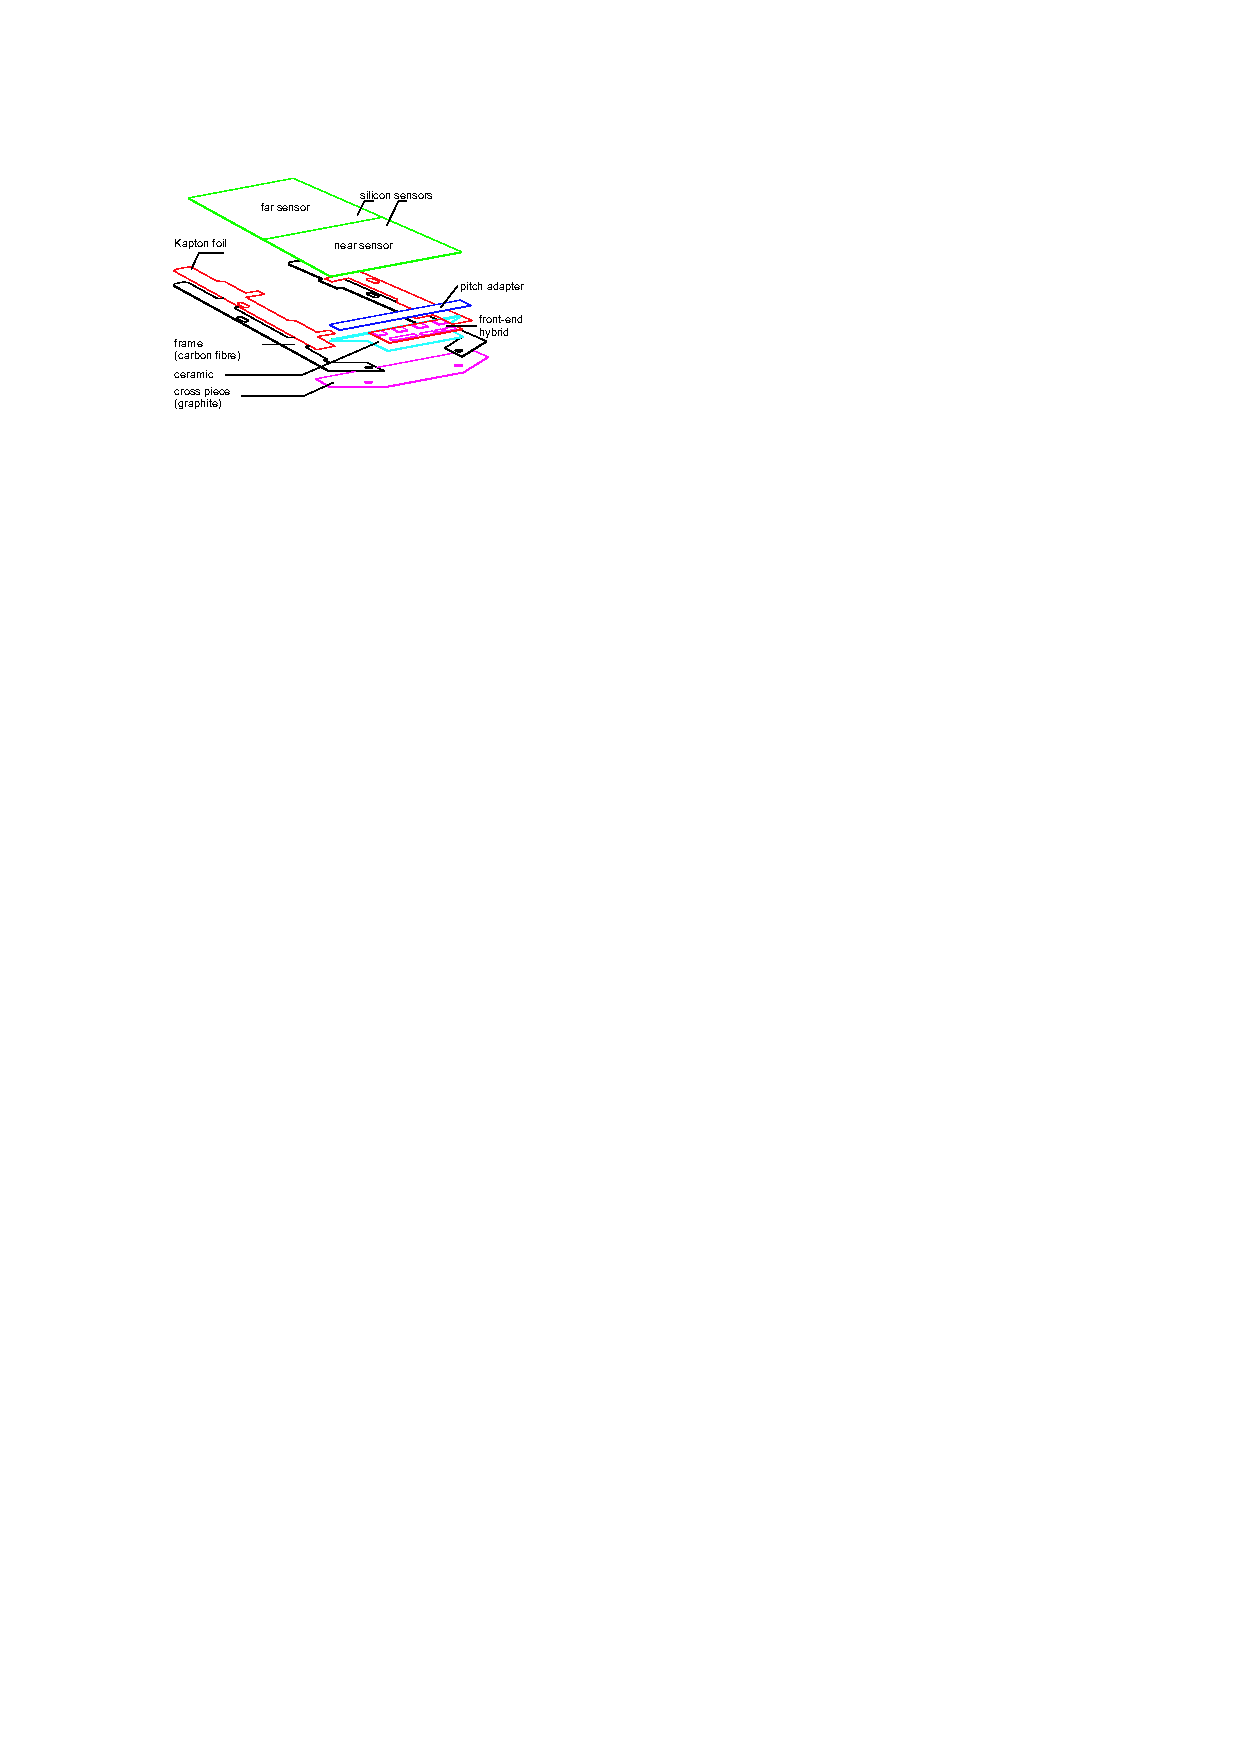
\includegraphics[scale=1.5]{tracker_module}
	\caption{Exploded view of a strip module with two sensors.  Reprinted from Fig. 3.22 of ref. \cite{1748-0221-3-08-S08004}.}
	\label{fig:tracker_module}
\end{figure}

\begin{figure}
	\centering
	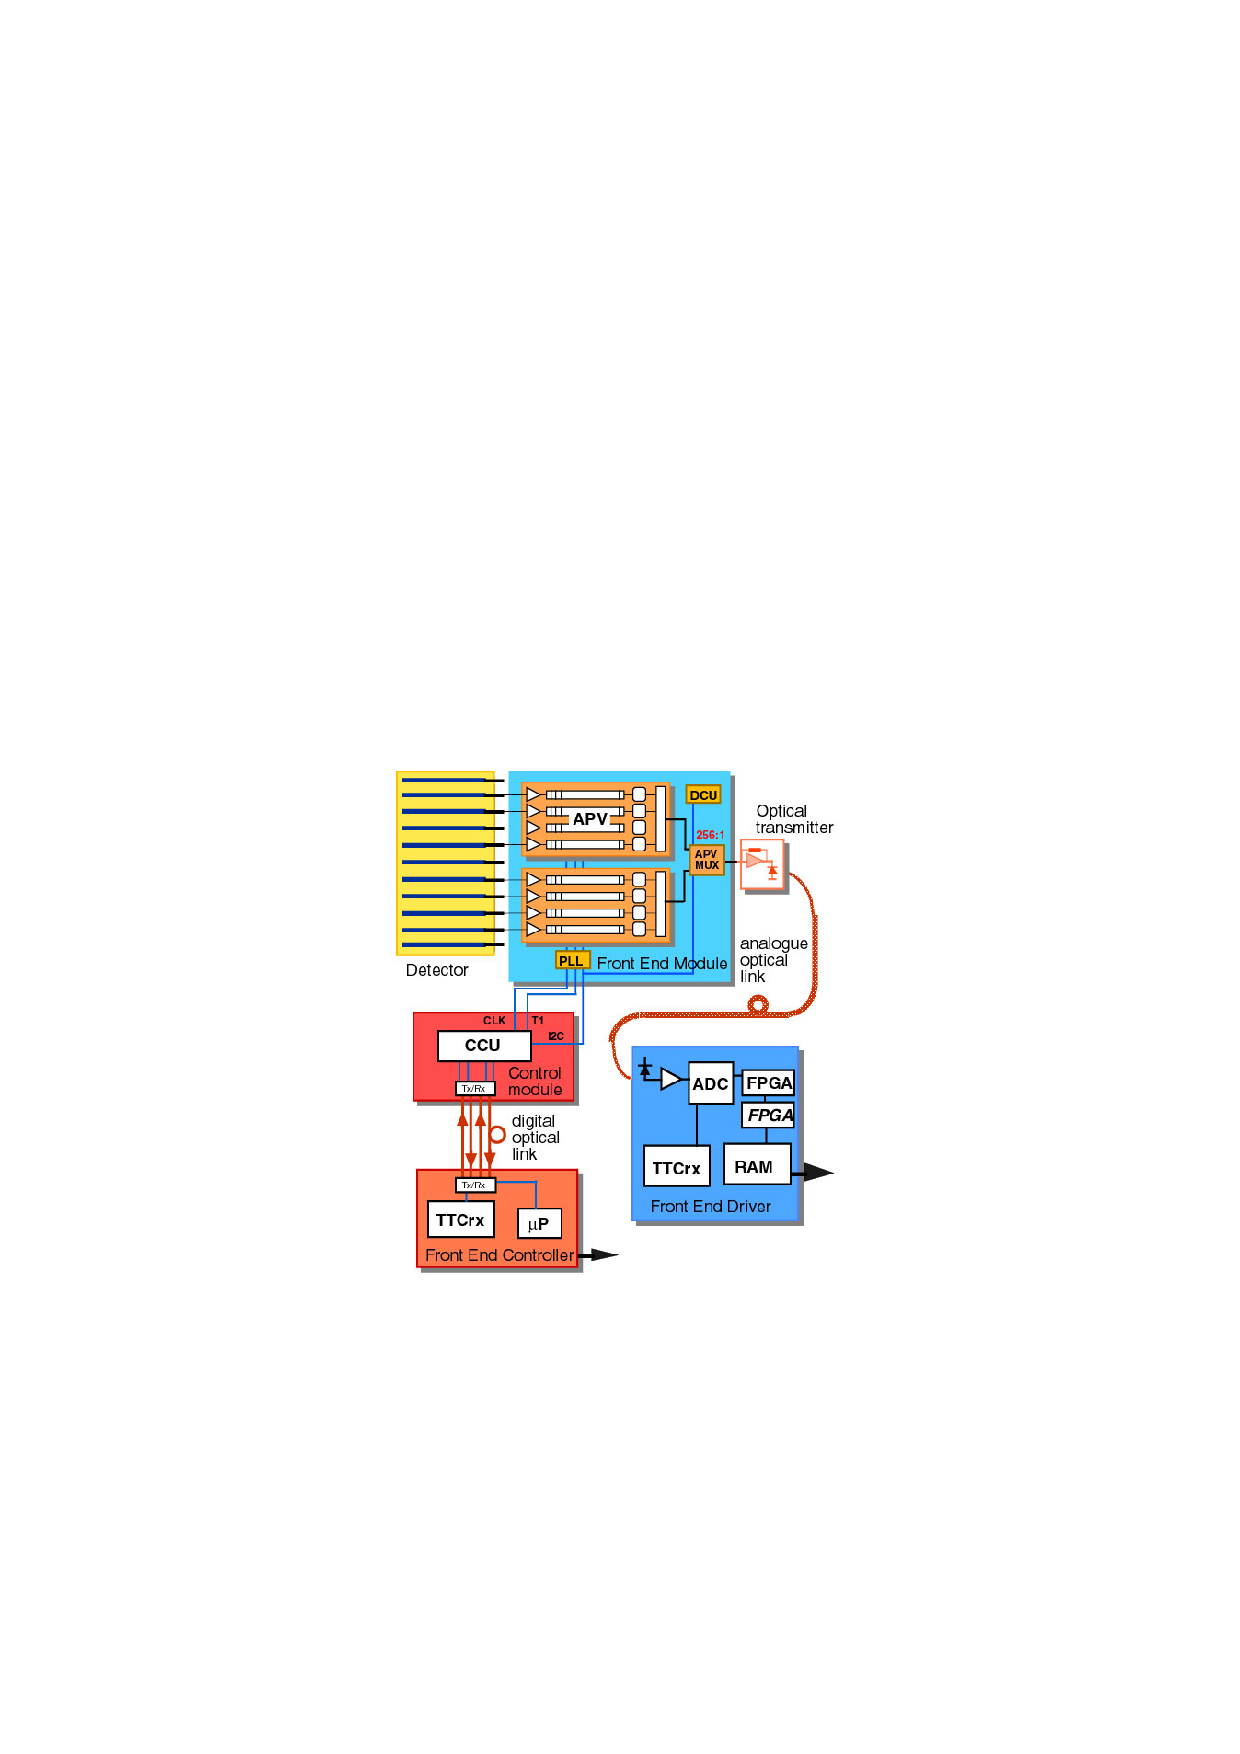
\includegraphics[scale=1.0]{tracker_readout}
	\caption{Block diagram of the strip readout architecture.  Reprinted from Fig. 3.20 of ref. \cite{1748-0221-3-08-S08004}.}
	\label{fig:tracker_readout}
\end{figure}

As an example of the strip capabilities, strip hit resolution and signal:noise measurements are shown in Figure~\ref{fig:tracker_results}.  The entire pixel + strip tracker has been used successfully in the reconstruction of primary and secondary vertices, electrons, muons, tau decays, and charm and bottom hadron decays.  In addition, the superior performance of the tracker over the hadronic calorimeter for low energy charged hadrons has been exploited in the the particle flow jet and \MET reconstruction technique (see Sec.~\ref{sec:Particle Flow}).  The CMS silicon strips, as well as the pixels, are well aligned and operating at close to design performance.  

\begin{figure}
	\centering
 	\subfloat[TIB signal:noise \cite{tracker_DPG_Twiki_TIB_SNR}.]{\label{fig:tracker_results_TIB_SNR}\includegraphics[scale=0.5]{tracker_results_TIB_SNR.gif}}
	\\
	\subfloat[TIB and TOB hit resolution as a function of strip pitch \cite{tracker_DPG_Twiki_res}.]{\label{fig:tracker_results_res}\includegraphics[scale=0.3]{tracker_results_res.gif}}
	\caption{Strip detector performance highlights.}
	\label{fig:tracker_results}
\end{figure}

\subsection{Electromagnetic Calorimeter}
\label{sec:Electromagnetic Calorimeter}

The electromagnetic calorimeter (ECAL) is composed of 75,848 lead tungstate ($\mbox{PbWO}_{4}$) crystals, divided into one barrel (EB) layer and two endcap (EE) disks.  In EB, there are 1700 crystals per \textit{supermodule} (SM), arranged in a $20\times85$ grid in $\phi\times\eta$.  Two SMs are laid out end-to-end to form one row at fixed $\phi$, with a total of 18 rows needed to cover the entire $2\pi$ extent in $\phi$.  The SMs may be operated independently.  In EE, the independent unit is a wedge-shaped sector, with nine sectors covering each endcap side.  The 14,648 EE crystals are divided approximately evenly between the 18 EE sectors.  A two-layer preshower detector is placed in front of the EE disks, each layer consisting of a lead absorber followed by 1.9 mm pitch silicon strip detectors (the strips in the first layer are rotated $90^{\circ}$ with respect to the second layer).  The ECAL layout is shown in Figure~\ref{fig:ECAL_layout}.

\begin{figure}
	\centering
	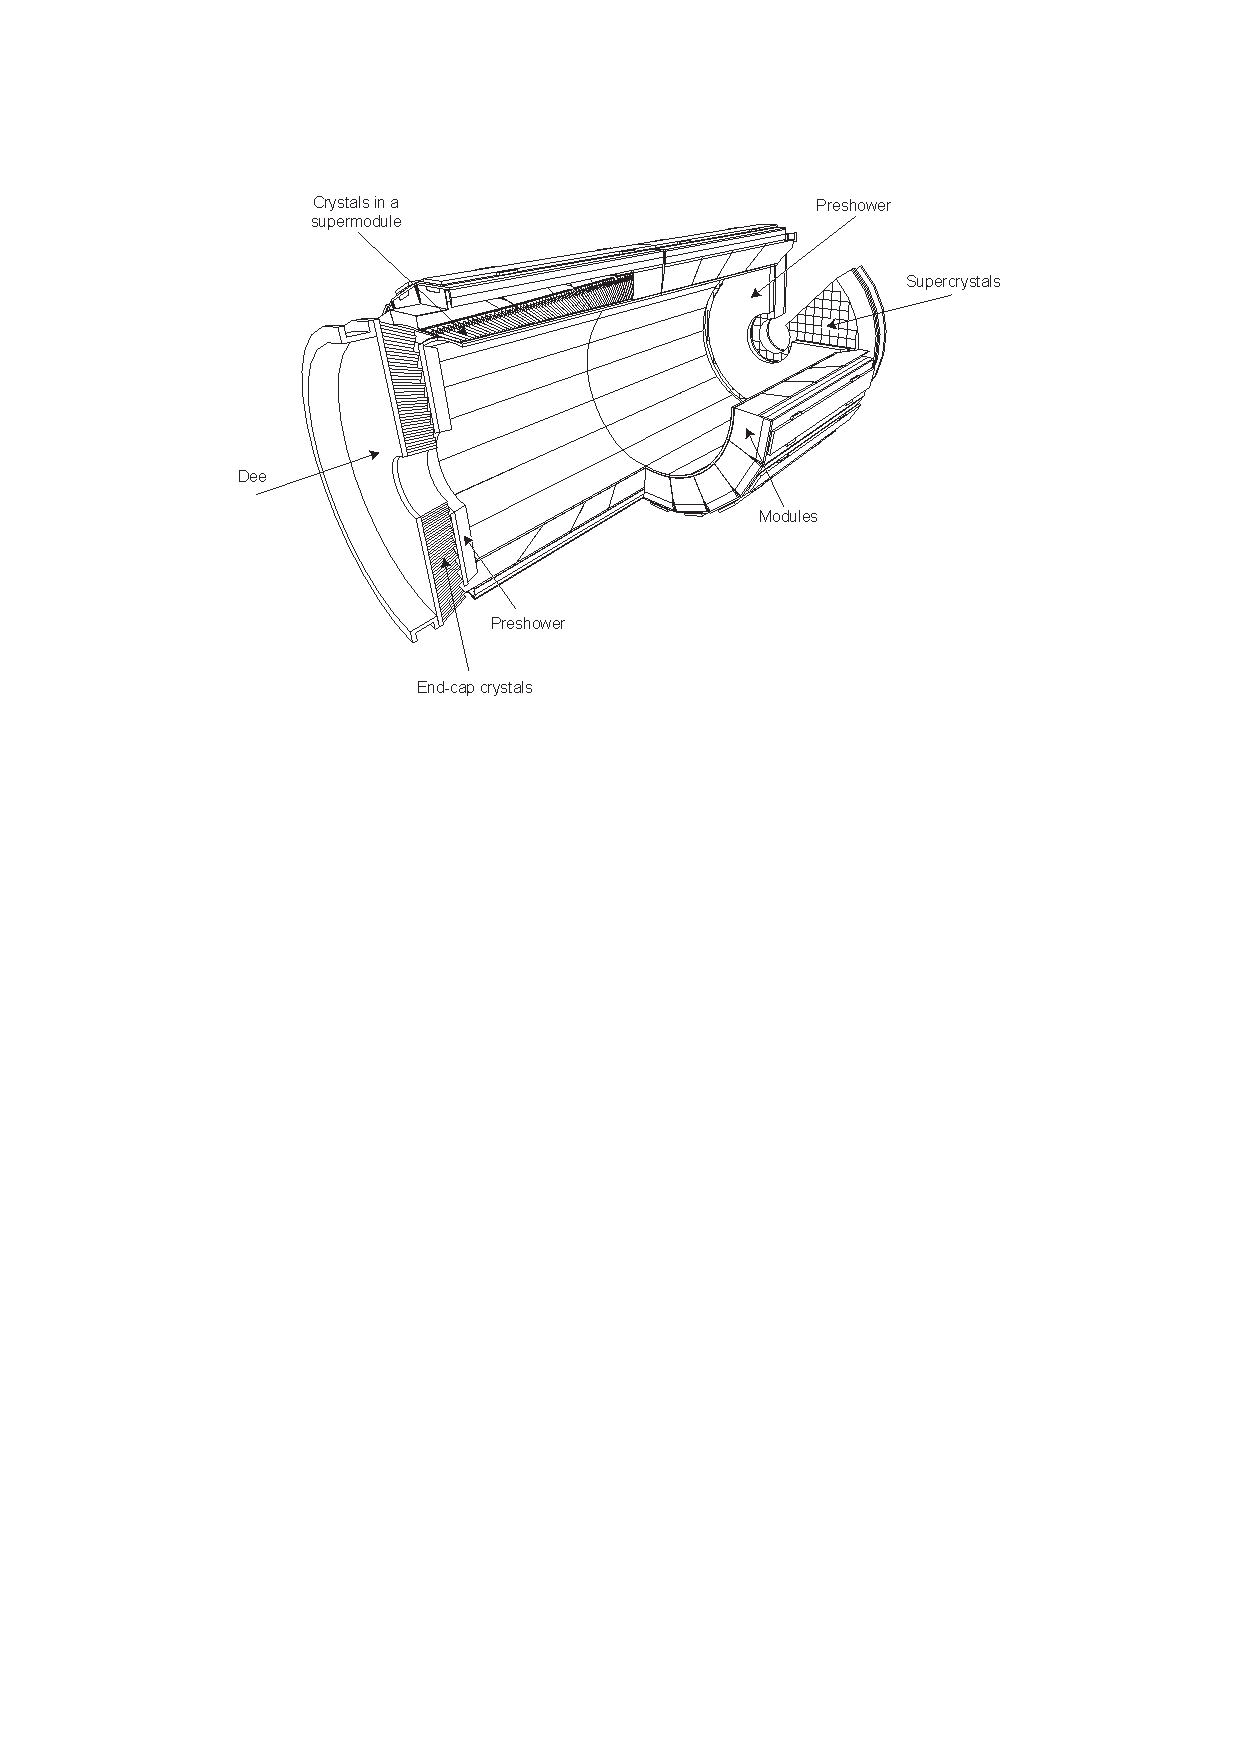
\includegraphics[scale=1.0]{ECAL_layout}
	\caption{Layout of the ECAL detector.  Reprinted from Fig. 4.5 of ref. \cite{1748-0221-3-08-S08004}.}
	\label{fig:ECAL_layout}
\end{figure}

The electromagnetic energy resolution can be parametrized as $(\sigma/E)^{2} = (S/\sqrt{E})^{2} + (N/E)^{2} + (C)^{2}$, where $S$ characterizes the size of photostatistical fluctuations, $N$ characterizes the contribution from electronics noise, and $C$ is a constant accounting for imperfect intercalibration between crystals, non-uniformity of crystal performance, and incomplete shower containment within one crystal.  The design goal of the ECAL is to achieve C = 0.5\%.  Therefore, fast, dense, and relatively radiation hard $\mbox{PbWO}_{4}$ was chosen as the crystal material.  When a photon or electron strikes the crystal, it initiates an electromagnetic (EM) shower.  Due to the density, short radiation length, and small Moli\`ere radius of $\mbox{PbWO}_{4}$, nearly the entirety of an EM shower can be contained in a single 23-cm long crystal with front face dimensions $2.2\mbox{ cm}\times2.2\mbox{ cm}$.  The crystals scintillate in the blue-green part of the spectrum at 440 nm, emitting $\sim80$\% of the scintillation light within 25 ns.  Light is transmitted along the length of the crystals and collected at the rear with avalanche photodiodes (APDs; semiconductor diodes) in EB or vacuum phototriodes (VPTs; conventional photomultipliers) in EE.  Since the light output is low and varies with temperature, the crystals must be kept precisely at $18^{\circ}$C.  The EB and EE crystals, which are slightly tapered to match the lateral shower development, are shown in Figure~\ref{fig:ECAL_crystals}.

\begin{figure}
	\centering
	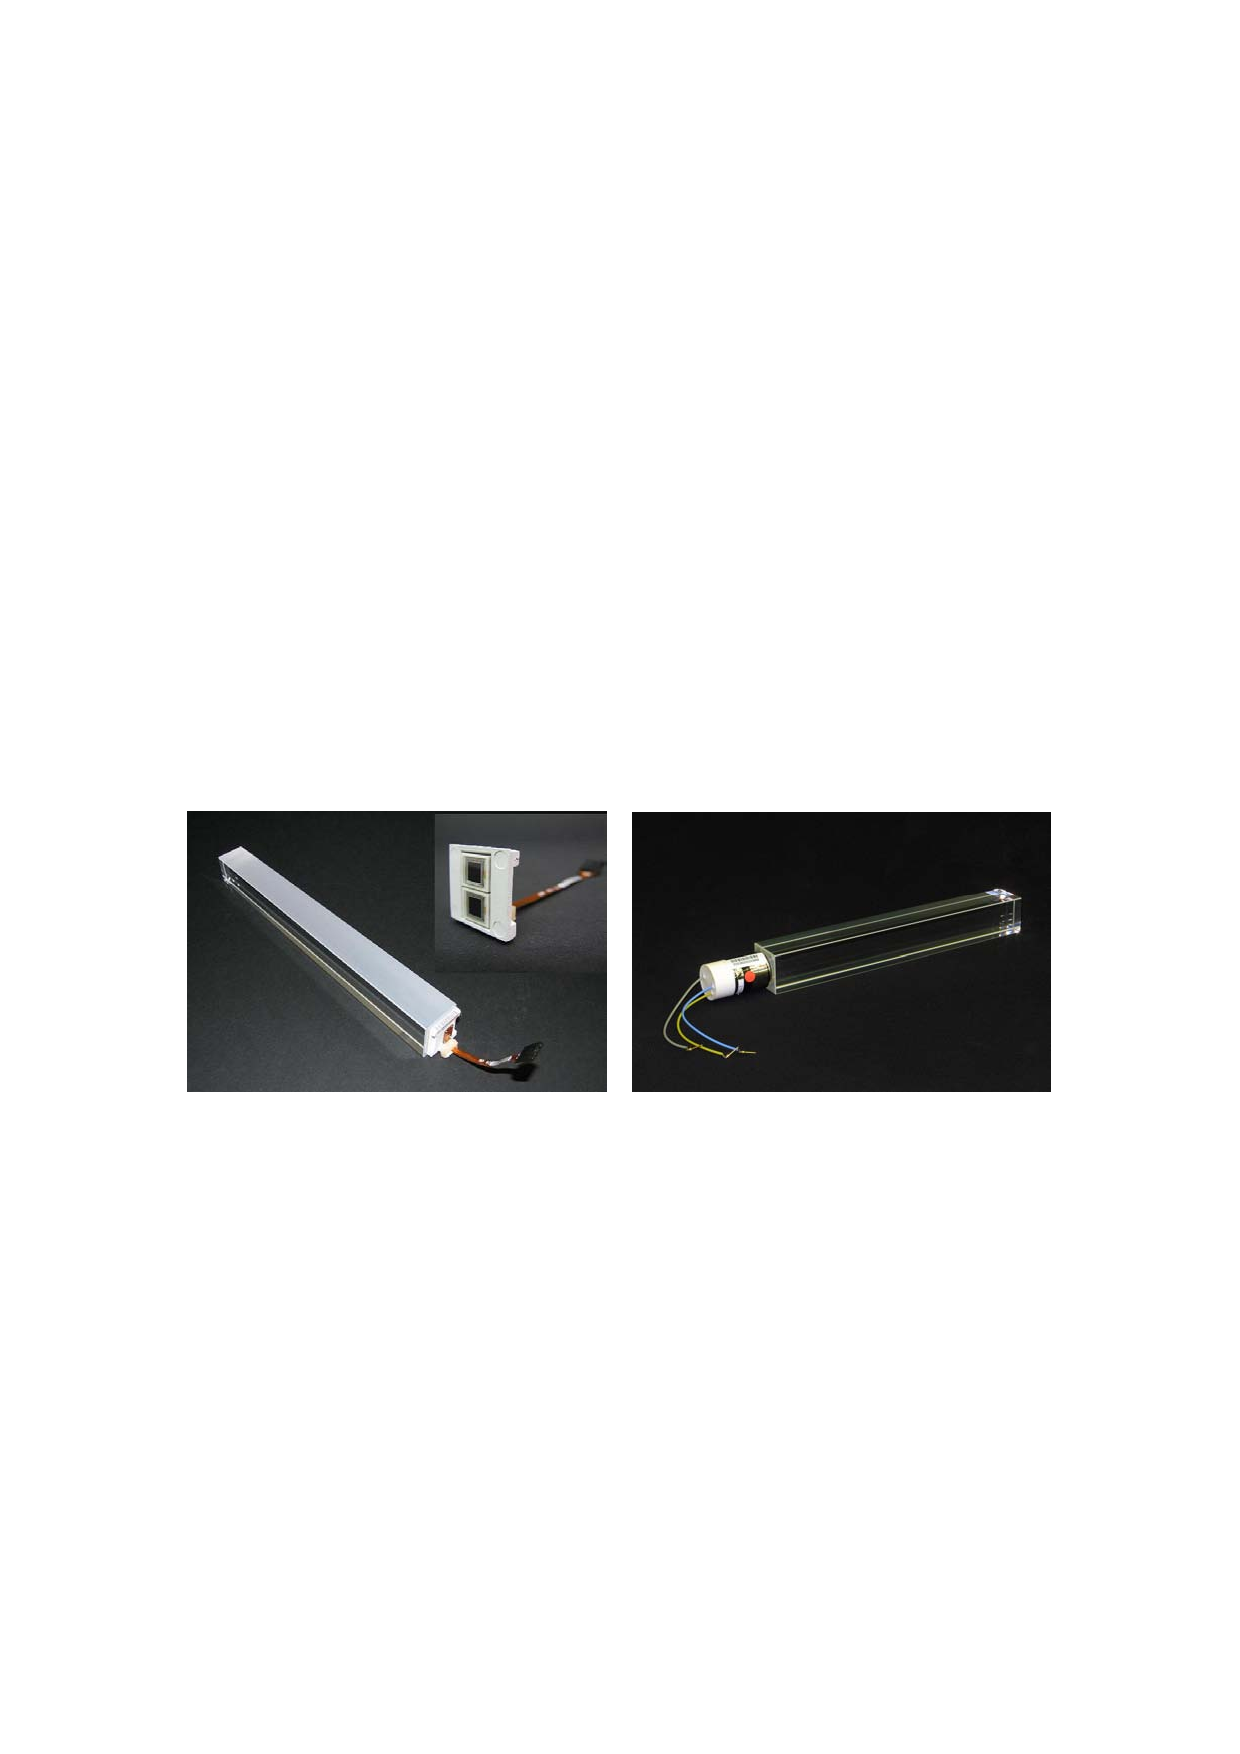
\includegraphics[scale=1.0]{ECAL_crystals}
	\caption{Left: EB crystal with attached APD.  Right: EE crystal with attached VPT.  Reprinted from Fig. 4.2 of ref. \cite{1748-0221-3-08-S08004}.}
	\label{fig:ECAL_crystals}
\end{figure}

For each trigger, 10 samples, each separated by 25 ns, are read out.  The 10-sample pulse is amplified and shaped by a multi-gain preamplifier (MGPA) residing on a very front end (VFE) card serving five crystals.  The MGPA can switch between gains 1, 6, and 12 to avoid saturation of the electronics, and affords a dynamic range up to 3 TeV.  The samples are digitized on the VFE card, then sent to the front end (FE) card serving five VFEs.  Digitized samples are buffered in the FE card until receipt of a trigger, when they are sent over an optical link to the data concentrator card (DCC) that interfaces to the global DAQ.  The DCC interfaces to the \textit{selective readout} processor, which decides whether a crystal should be read out with or without zero suppression based on its proximity to a high-energy hit.  The clock is transmitted to the FE cards from the Clock and Control System (CCS) boards.  A flow chart of the crystal readout is given in Figure~\ref{fig:ECAL_readout}.

\begin{figure}
	\centering
	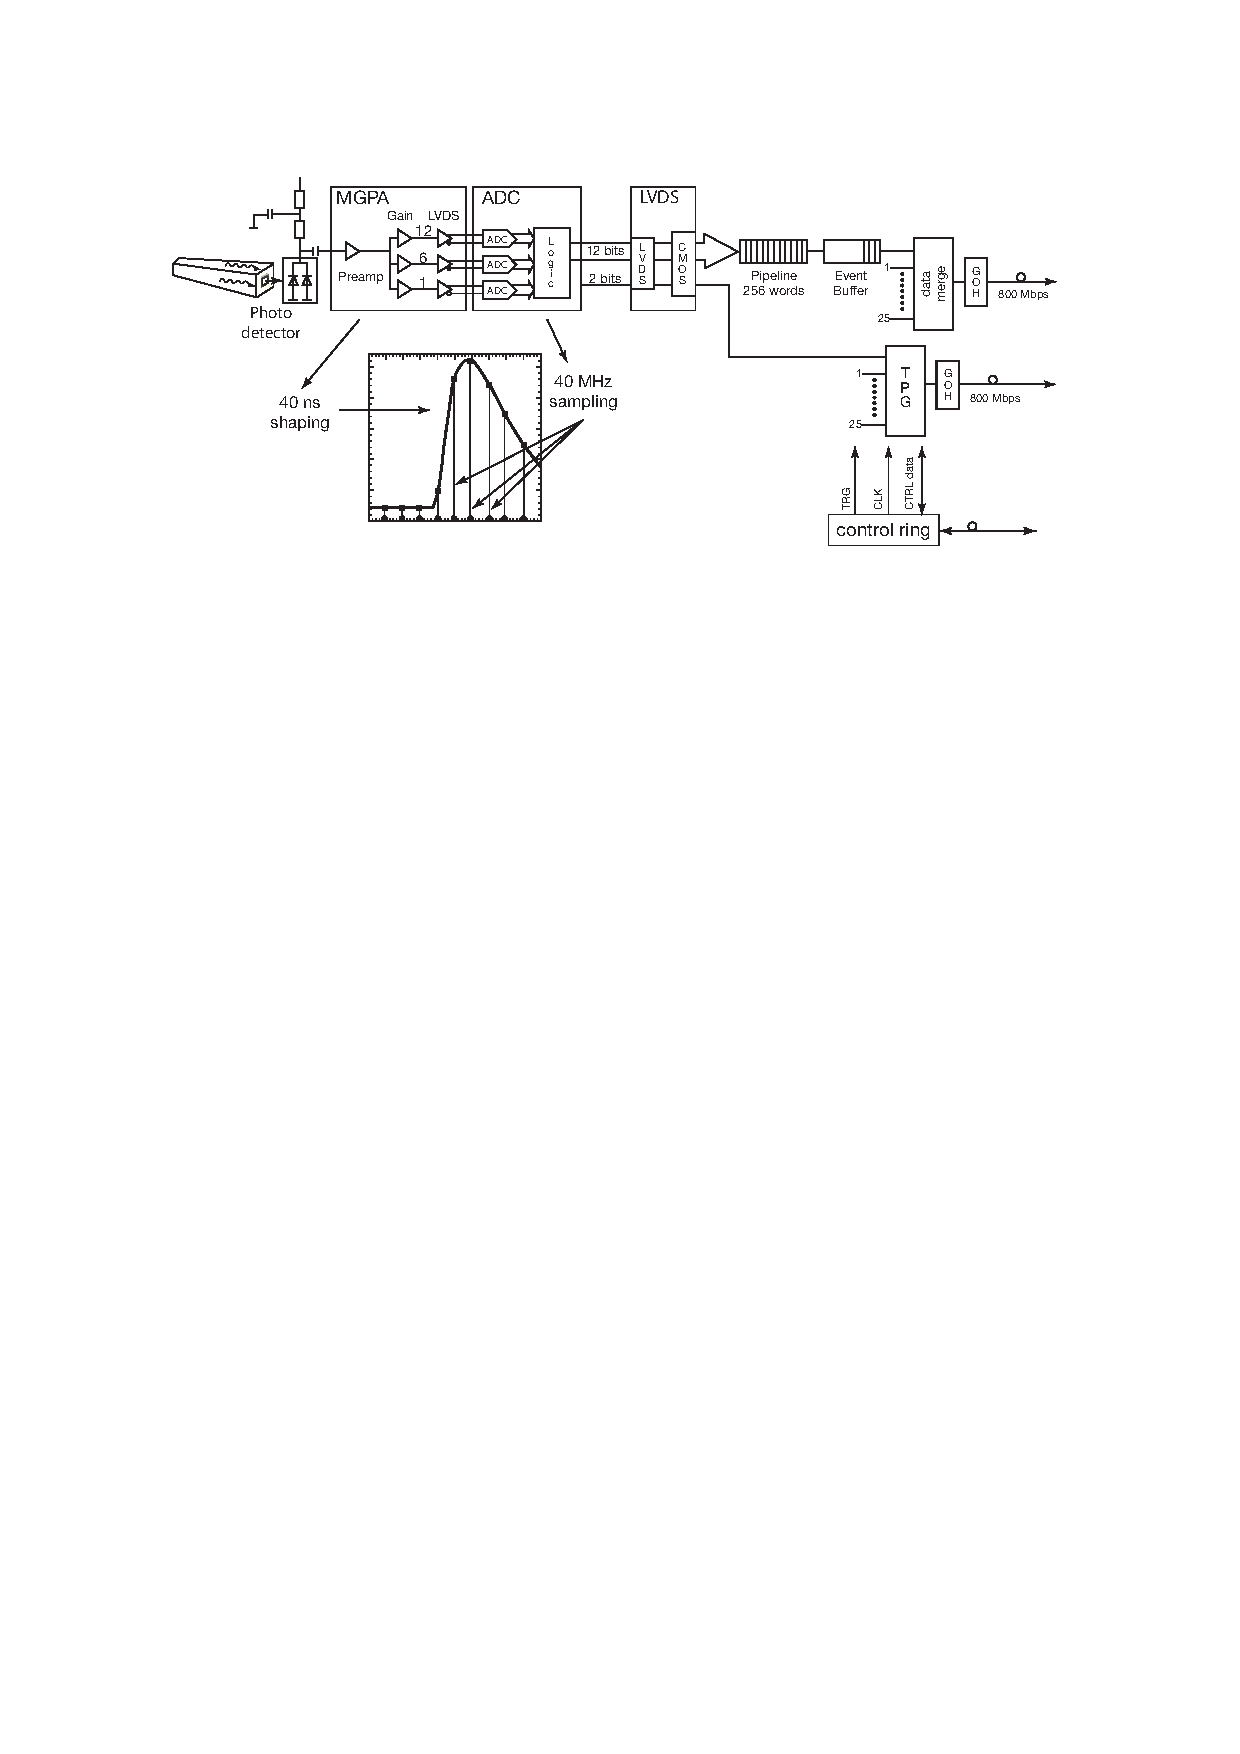
\includegraphics[scale=1.0]{ECAL_readout}
	\caption{Flow chart of the crystal readout, showing the 10-sample pulse shape.  Reprinted from Fig. 4.9 of ref. \cite{1748-0221-3-08-S08004}.}
	\label{fig:ECAL_readout}
\end{figure}

At each bunch crossing, the trigger concentrator cards (TCC) of the ECAL compute \textit{trigger primitives} from $5\times5$ non-overlapping transverse energy sums (in the endcaps the geometry is not always $5\times5$).  This information, along with a special bit in EB only characterizing the transverse shower profile that is used for rejection of anomalous APD hits (see Sec.~\ref{sec:Calibrated EB/EE Hits}), is transmitted from the TCCs to the synchronization and link boards (SLBs), and then on to the global trigger system.  The trigger decision is communicated to the DCCs, which request the buffered data from the front ends if the decision is affirmative.

Despite the radiation hardness of lead tungstate relative to other types of crystals, it still suffers from transparency loss due to radiation-induced lattice damage, as shown in Figure~\ref{fig:ECAL_rad_damage}.  In addition, any unforeseen change in the gains of the MGPAs and VPTs, or in the pedestal levels, will degrade the energy resolution.  For this reason, a continuously running calibration system is installed with the ECAL.  The system makes use of the LHC abort gaps to read out the pedestal levels, test pulses fired into the MGPAs, and laser (EB and EE) or LED (EE only) pulses fired into the crystals at regular intervals.  Laser and LED events are used to compute corrections to the crystal gains for transparency loss, while the other types of calibration events serve to monitor changes in the electronics performance due to magnetic field or high voltage cycling.  The mean time between transparency measurements is $\sim40$ minutes.  Figure~\ref{fig:ECAL_laser_system} shows the architecture of the laser monitoring system.  The additional EE light monitoring system consisting of LEDs serves to (a) stabilize the response of the VPTs and (b) corroborate the laser calibration measurements.  I describe it here in some detail because it is my principal contribution to the CMS detector.

\begin{figure}
	\centering
	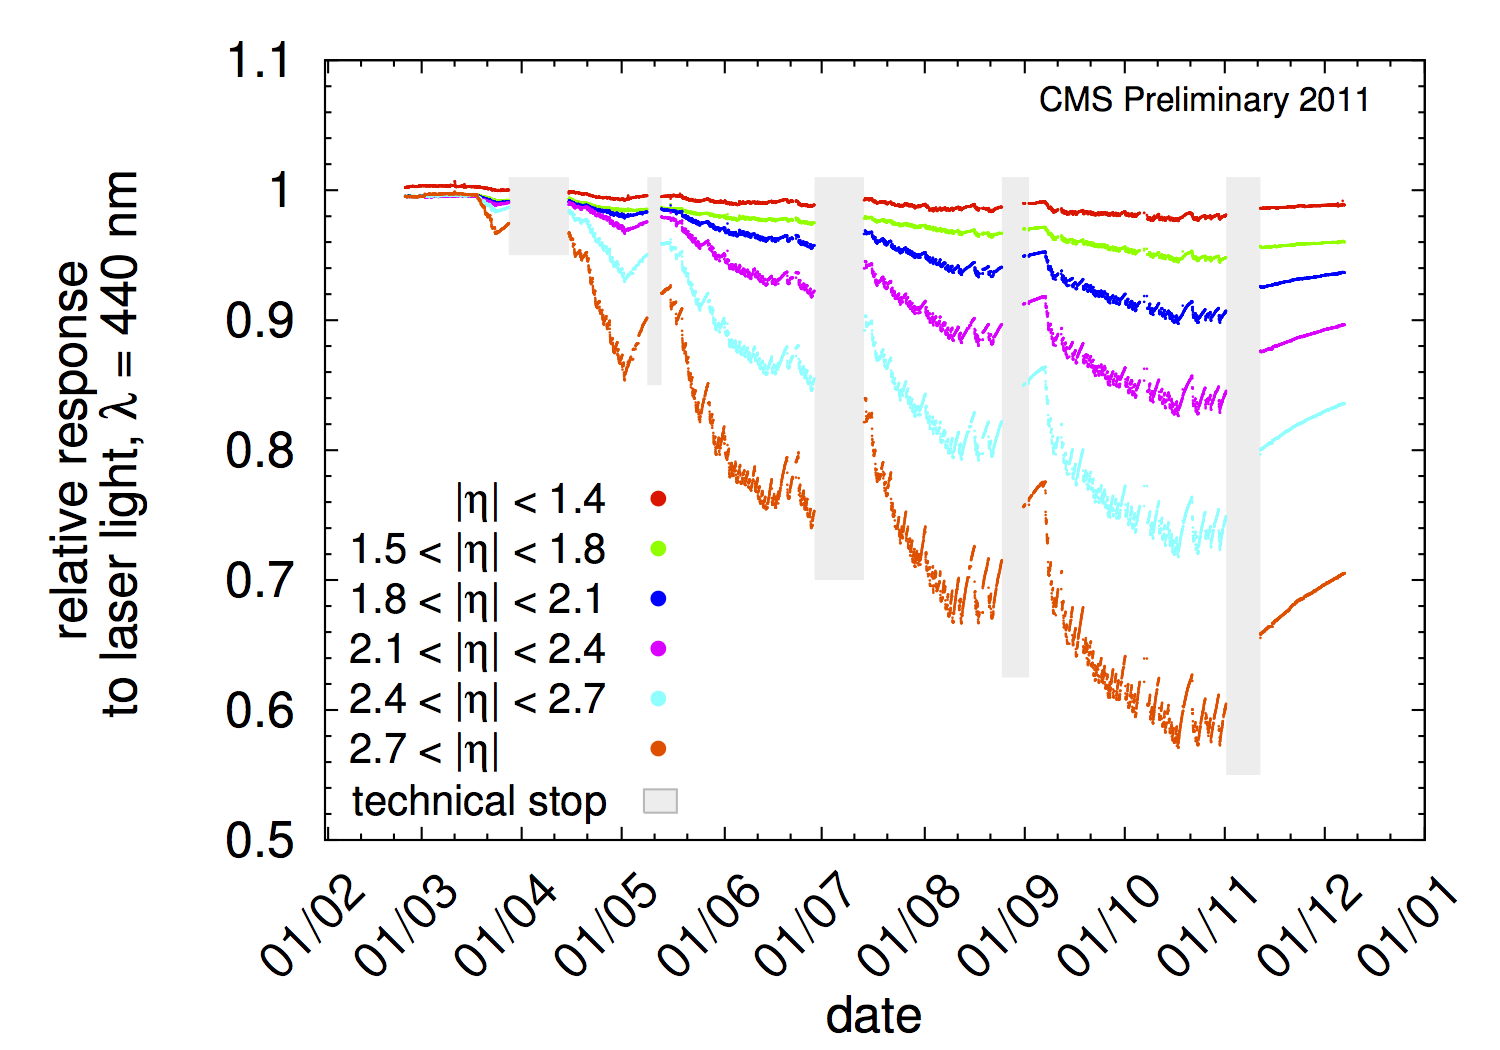
\includegraphics[scale=1.0]{ECAL_rad_damage}
	\caption{Relative response of the crystals to blue laser pulses from February 1, 2011 to January 1, 2012 \cite{ECAL_DPG_Twiki_rad_damage}.  Technical stops, during which the LHC is turned off for maintenance and development, are shown in gray.  These periods of inactivity correspond to growth in the crystal response, as radiation damage recovery occurs.}
	\label{fig:ECAL_rad_damage}
\end{figure}

\begin{figure}
	\centering
	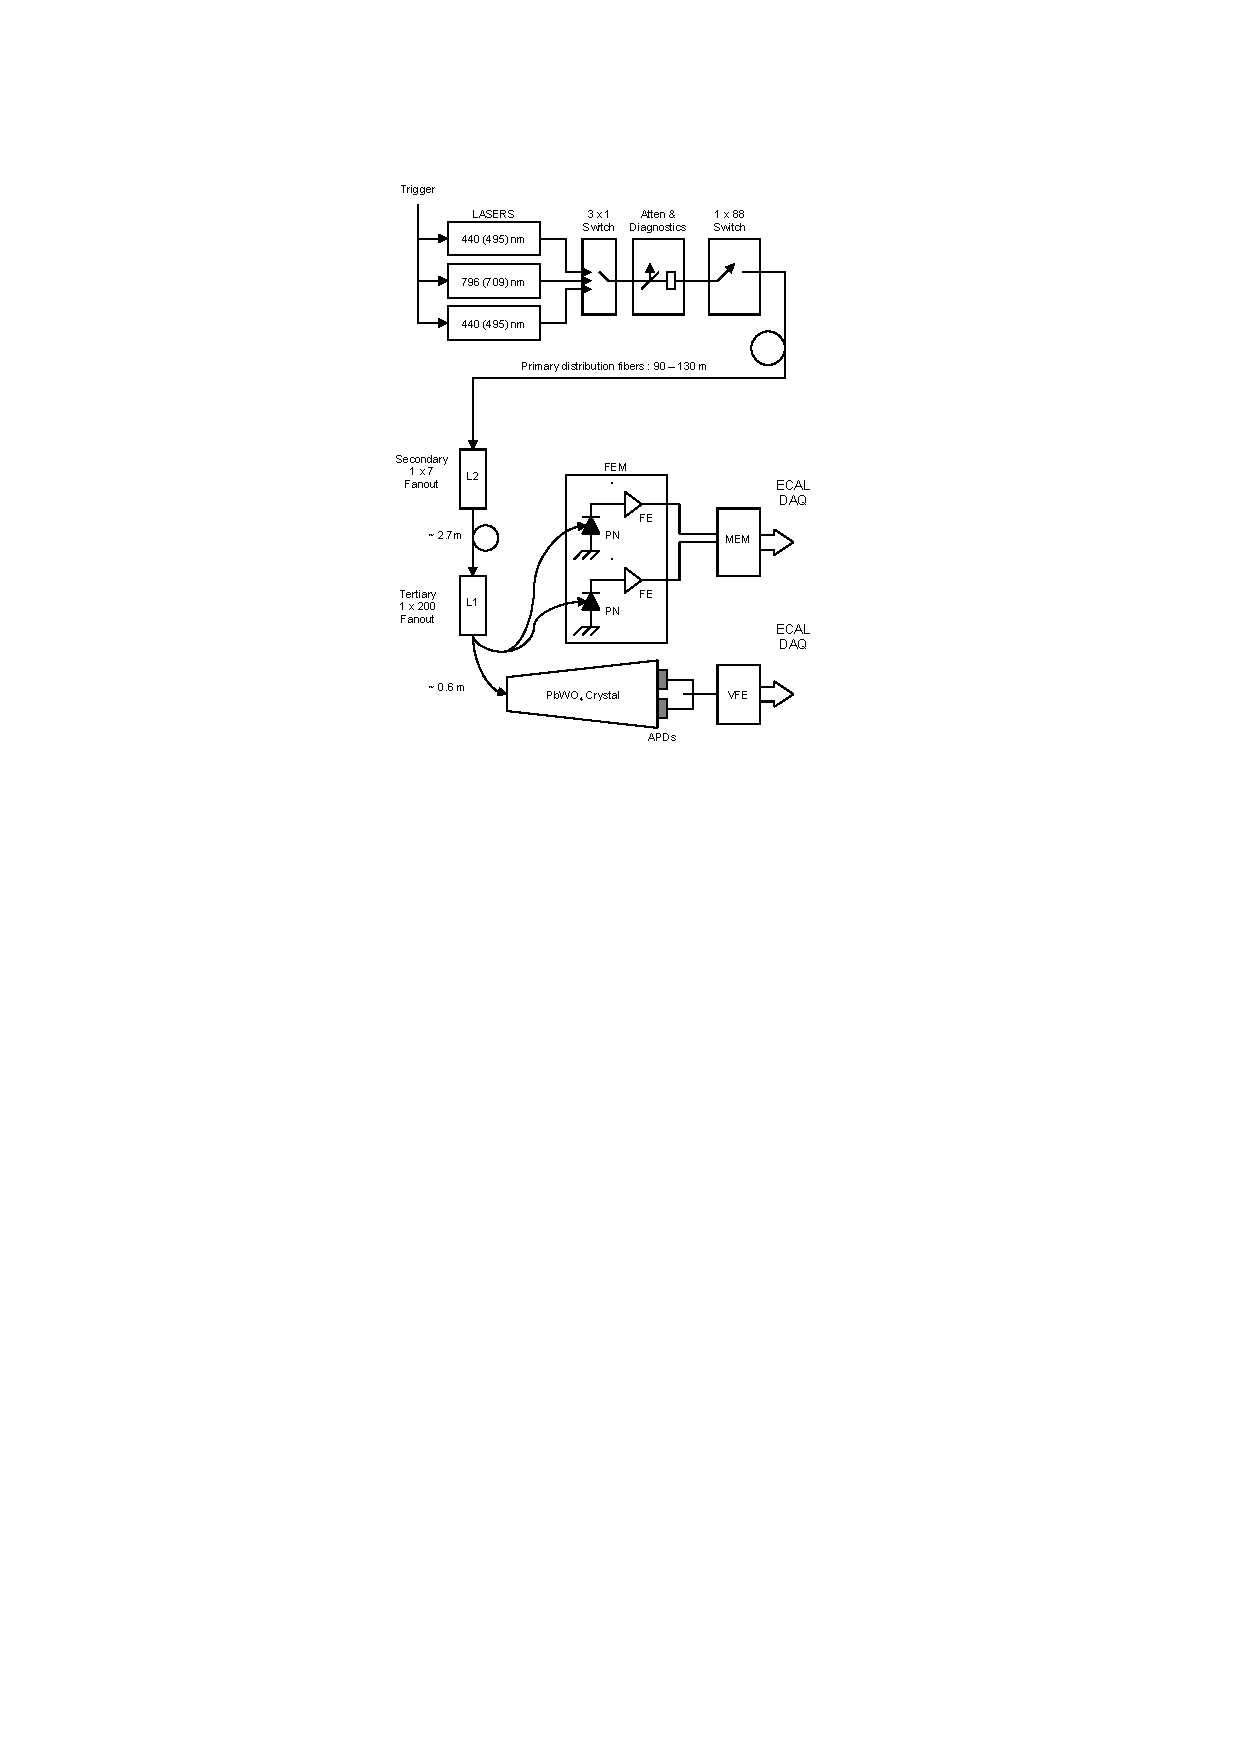
\includegraphics[scale=1.0]{ECAL_laser_system}
	\caption{Architecture of the laser monitoring system.  Reprinted from Fig. 4.16 of ref. \cite{1748-0221-3-08-S08004}.}
	\label{fig:ECAL_laser_system}
\end{figure}

VPT gains are known to be sensitive to the frequency and amplitude of incident light \cite{Akopdzhanov1979247}.  In general, as the pulsing frequency increases the gain decreases and vice versa, but some VPTs may exhibit a different dependence on rate changes.  The gain changes are most abrupt when a source of pulsed light (i.e. the LHC) is suddenly turned on or off.  Deviations of a few percent to over ten percent have been observed in the lab (see Figure~\ref{fig:VPT_gain_changes}).  The EE LED system mitigates the effects of LHC beam injections and dumps on the stability of the VPTs by continuously providing light pulses to the VPTs, irrespective of the state of the beam.  At LHC on/off transitions, the frequency change seen by the VPTs is therefore less severe due to the continuous presence of the background LED pulse, leading to a reduced change in gain.  Note that although the VPT effect is strongly suppressed in the 3.8 T magnetic field of CMS, the LED system is still required in light of the stringent requirements on ECAL stability imposed by the $C = 0.5\%$ resolution goal.  At present, there is no indication of a significant VPT effect discernible on top of the radiation damage, but in the future improved calibration precision will demand control over small effects like VPT gain fluctuations.

\begin{figure}
	\centering
	\includegraphics[scale=0.7]{on_off-1_graph}
	\caption{Change in response of nine different VPTs in zero magnetic field vs. time.  The response of each VPT is normalized to its response for the earliest data point taken.  For times less than 0, no light pulsing is applied to the VPTs.  For times between 0 and 20 minutes, pulsed LED light was applied to the VPTs.  For times later than 20 minutes, the pulsing source was again removed.}
	\label{fig:VPT_gain_changes}
\end{figure}

In addition to their stabilizing effect, the LED pulses are also read out as part of the ECAL calibration cycle and used to correct for crystal transparency loss and VPT gain loss due to aging.  Figure~\ref{fig:VPT_aging} shows the decrease in response of a VPT in the lab at 3.8 T as a function of integrated charge at the VPT photocathode.  The loss of response due to photocathode aging differs from VPT to VPT, but a typical value is $\sim25\%$ per 0.05 C of integrated charge.  The intrinsic time stability of LEDs (sub-percent) over the laser (few percent) used for ECAL calibration makes the LED information very useful despite the smaller light intensity delivered.  LED data are used to correct for transparency loss and VPT aging whenever laser data are missing due to technical problems.

\begin{figure}
	\centering
	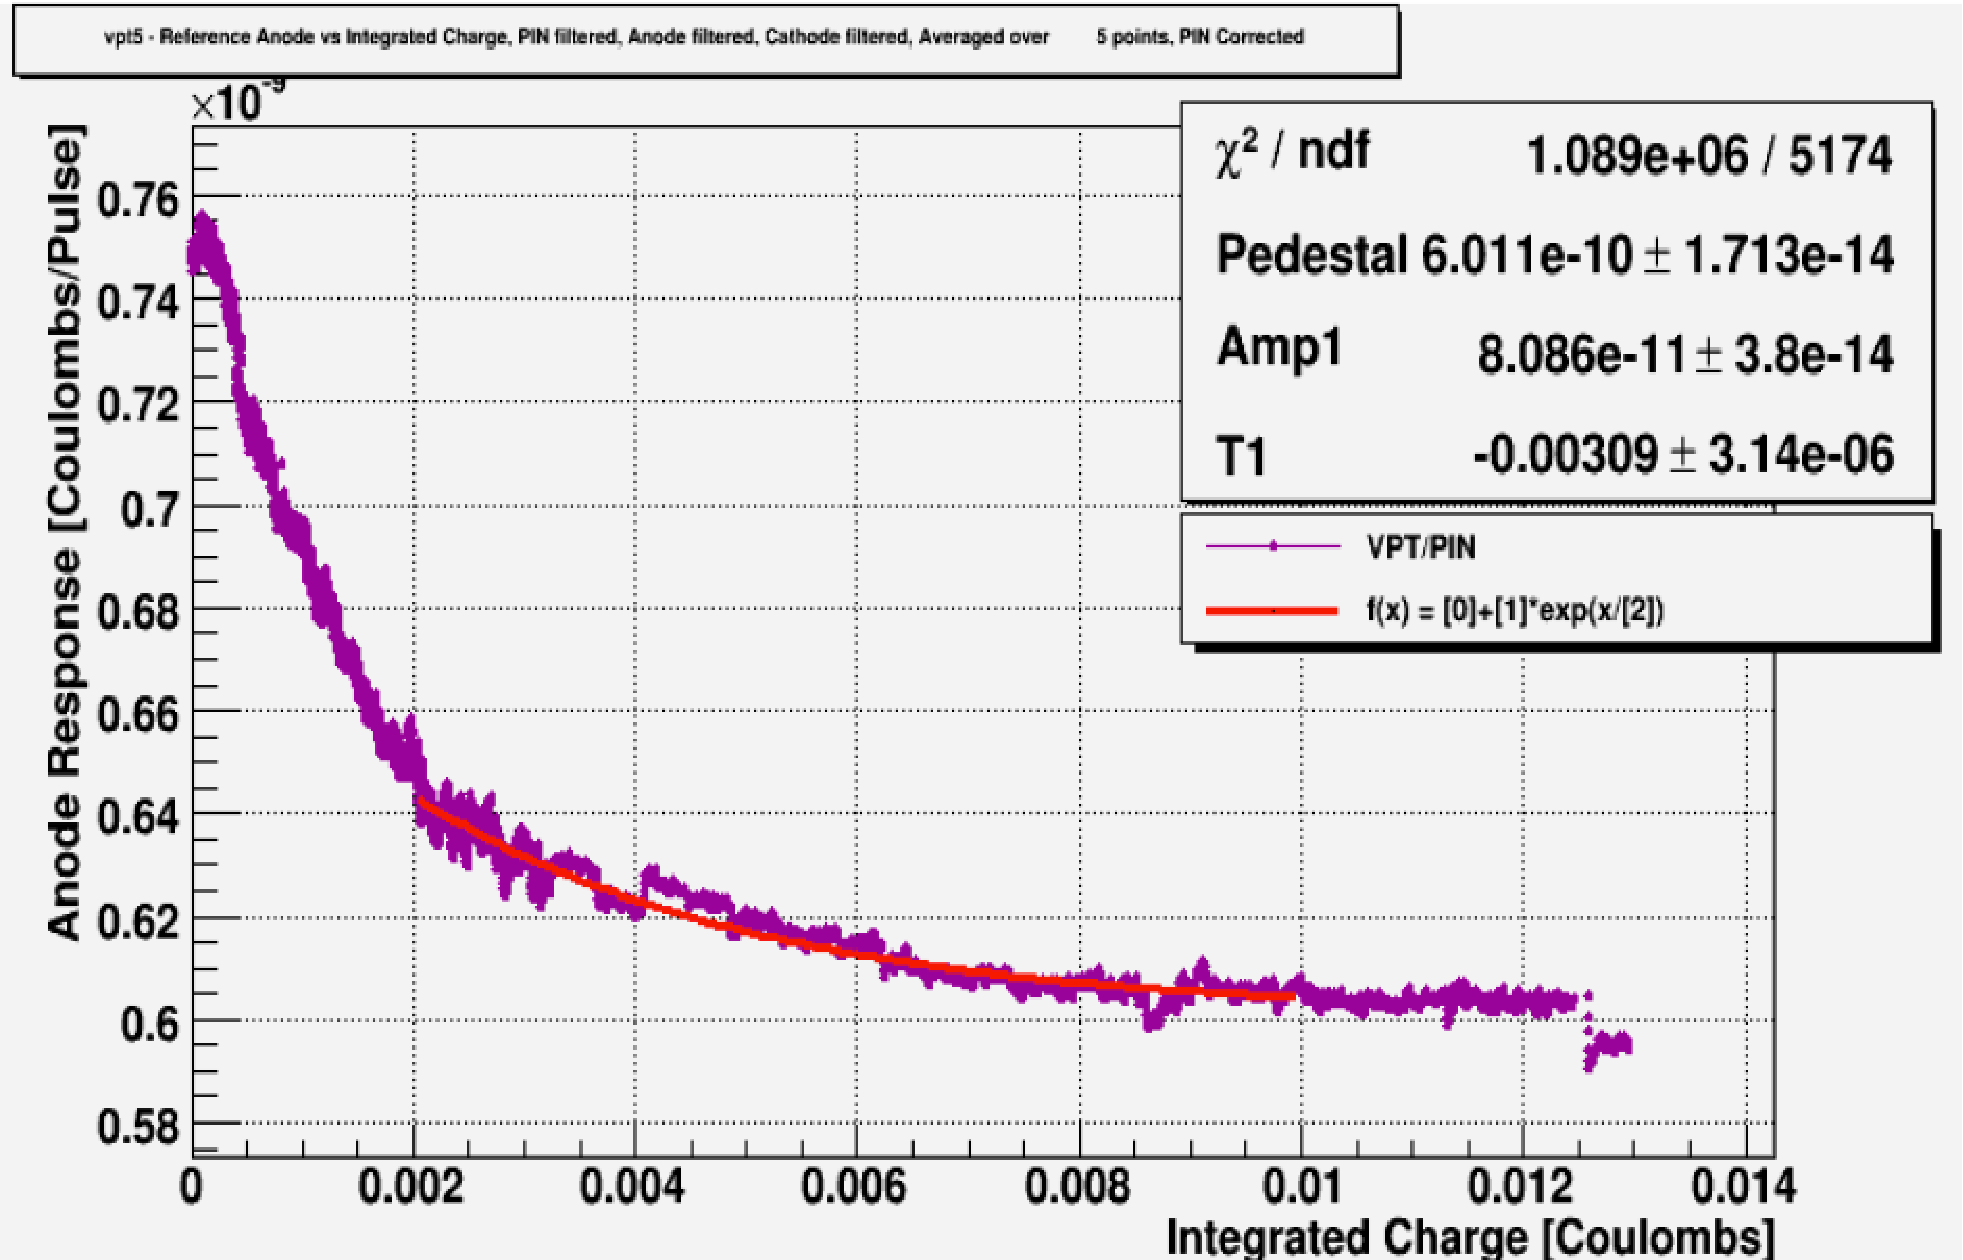
\includegraphics[scale=0.375]{VPT_aging}
	\caption{VPT response in a 3.8 T laboratory magnetic field to blue LED light vs. integrated charge at photocathode \cite{Wood}.  The response is corrected for changes in the LED light output by PIN diode normalization.  For integrated charge less than $\sim0.003$ C, the average current draw at the photocathode is $\sim1$ nA, delivered by blue LED triggered at 2 kHz.  For integrated charge greater than $\sim0.003$ C, the average current draw is $\sim10$ nA from a 20 kHz trigger rate.}
	\label{fig:VPT_aging}
\end{figure}

The LED system utilizes two wavelengths.  Blue LEDs, at 450 nm wavelength, are near the peak of the crystal scintillation and VPT photocathode efficiency, and therefore are ideal for transmitting the maximum amount of light to VPTs for stability pulsing.  Orange LED light, at 617 nm wavelength, is transparent to the crystals but still somewhat efficient for the VPT photocathode, allowing loss of response from crystal damage to be disentangled from VPT gain changes.  In addition, the orange wavelength serves as a second calibration wavelength in EE, where there is only a blue laser.  Each endcap disk holds 38 LED circuits, with each circuit driving four blue and three orange LEDs.  Each of the seven LEDs of a circuit is coupled to the same diffusing sphere by an optical fiber whose cleaved end is stuck inside a hole drilled into the LED surface.  The light entering the diffusing sphere is fanned out to $\sim200$ crystals + two PN diodes for tracking of the stability of the LED itself.  A diagram of the inputs and outputs of a single diffusing sphere is shown in Figure~\ref{fig:LED_DS_diagram}.  38 diffusing spheres cover a single endcap disk.

\begin{figure}
	\centering
	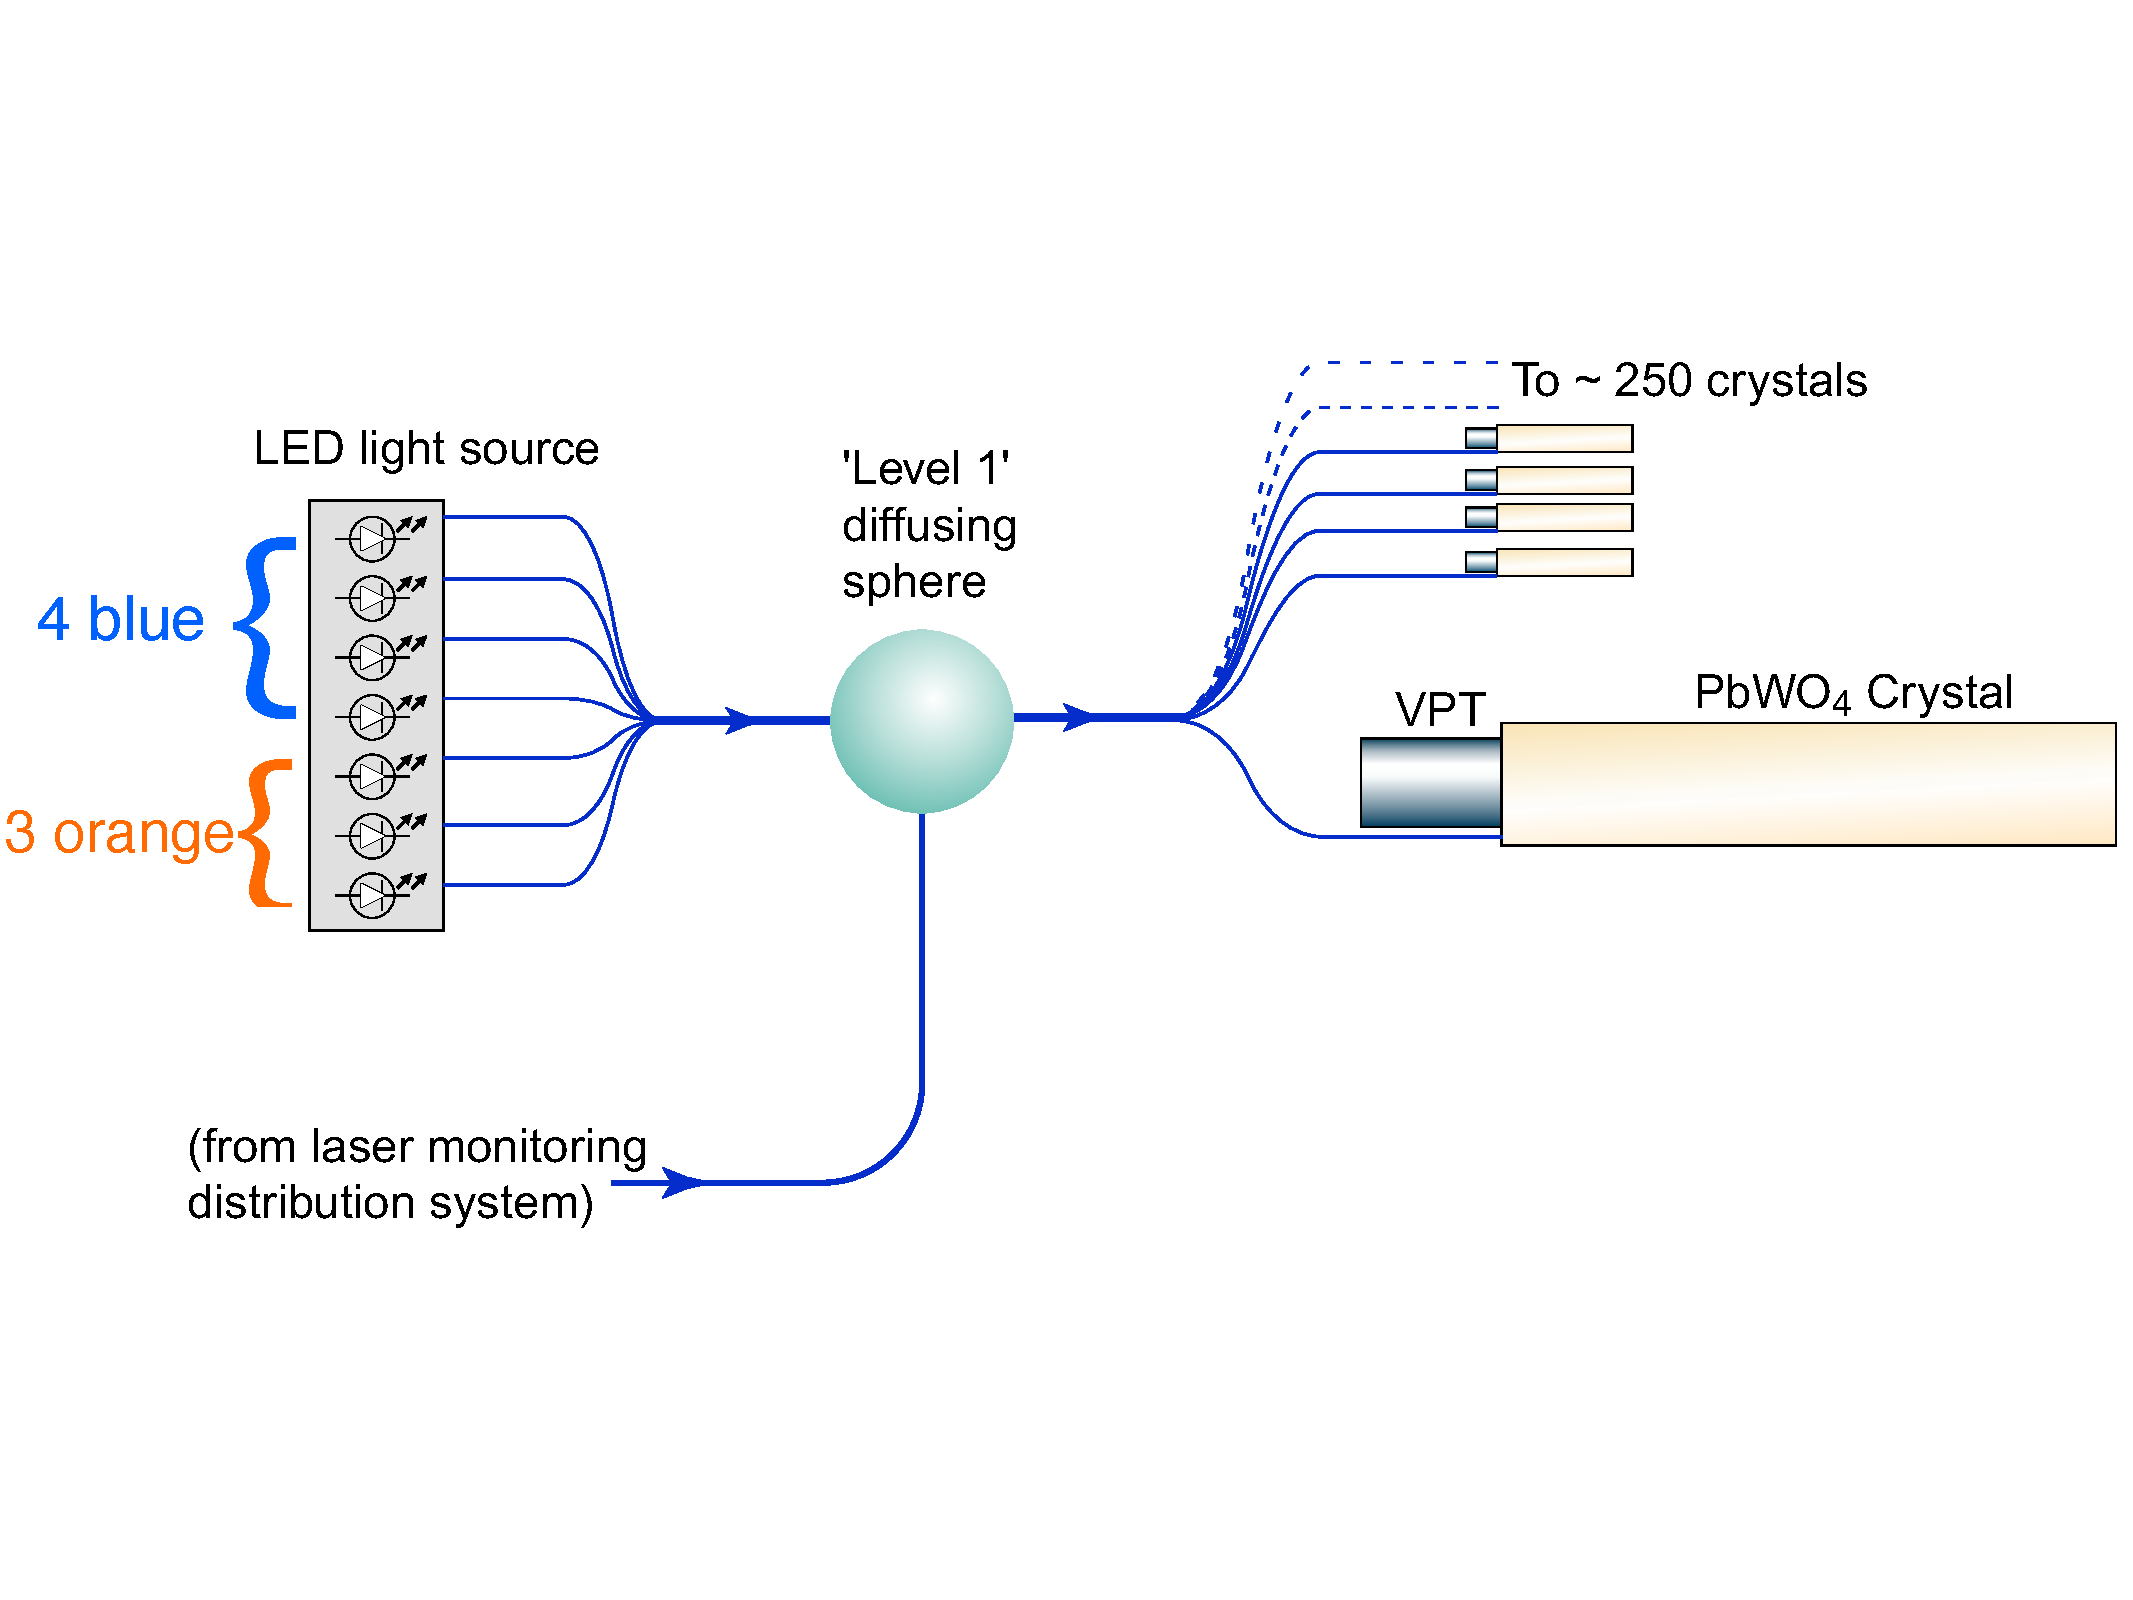
\includegraphics[scale=0.375]{LED_DS_diagram}
	\caption{Diagram of the LED inputs to a diffusing sphere and the fanout to the crystals.  Adapted from Fig. 4.8 of ref. \cite{1748-0221-3-08-S08004}.}
	\label{fig:LED_DS_diagram}
\end{figure}

The LED driver circuits are grouped into boxes that serve six, four, or three diffusing spheres each, for a total of four boxes per half-endcap ``dee" (eight per disk).  Each box is powered from supplies residing in the underground control room at Point 5.  One power supply channel feeds four LED boxes.  The four boxes per dee receive a common clock signal and LED pulse trigger from a control box in the underground control room.  The amplitude of a group of four blue or three orange LEDs is controlled by a single digital-to-analog converter (DAC) chip.  For the blue LED groups, the amplitude ranges from zero to $\sim50$ GeV equivalent.  Due to the lower photocathode efficiency for orange light, the amplitude of orange groups ranges from zero to $\sim5$ GeV equivalent.  Power distribution, LED amplitudes, and pulse widths and delays are set by a computer program that interfaces to the hardware via an Ethernet-to-serial converter.  The hardware setup of the LED system is shown in Figure~\ref{fig:LED_hardware}.

\begin{figure}
	\centering
	\includegraphics[scale=0.375]{LED_control_and_monitoring}
	\caption{Hardware setup of the LED system.}
	\label{fig:LED_hardware}
\end{figure}

The LED system has two modes: calibration, in which both blue and orange LED pulses are read out and processed for calibration purposes; and stability, in which blue LED pulses are fired continuously but not read out.  During a calibration cycle, the LED system is in stability mode except during the calibration mode readout periods.  For a given EE wedge, these calibration periods occur approximately every 40 minutes and last $\sim6$ seconds.  Orange or blue LED triggers are read out during the calibration periods.  Once they end, the EE wedge returns to stability mode.  Critically, stability pulsing occurs both inside and outside of a CMS data taking run, insuring the stability of the VPTs.  The calibration and stability pulsing rates, as well as the overall health of the LED hardware, is monitored every ten minutes.

Calibration and stability triggers come once per LHC abort gap (see Sec.~\ref{sec:Beam Injection}).  The calibration trigger readout rate is always 100 Hz, corresponding to a trigger every 114 abort gaps, while the stability pulsing rate can range between 100 Hz and 11.4 kHz (corresponding to a trigger every abort gap) in steps of 100 Hz.  The stability pulsing rate cannot go below 100 Hz (unless it is exactly 0 Hz) because the pulse itself is generated upon receipt of a calibration trigger.  For calibration events, the entire 119-bunch-crossing long abort gap is dedicated to calibration triggers.  However, in the rest of the abort gaps, only the last 35 bunch crossings of the gap are reserved for LED stability pulses.  This arrangement allows the rest of the abort gap to be used to search for long-lived exotic particles decaying at random with respect to the LHC collision frequency \cite{PhysRevLett.106.011801}.  A very small portion of the tail of the triggered VPT pulse ``leaks" into the first few bunch crossings of the orbit following the abort gap, leading to an increase in the pedestal level of $\sim0.7$ ADC counts (compared to a noise level of $\sim2$ ADC counts).

Transitions between calibration and stability modes are executed by selectively zeroing the amplitudes of certain LED groups and maximizing the amplitudes of others.  The computer program that controls the DACs of the LED system is itself controlled by a server running on a dedicated PC at Point 5.  This server listens to commands from a program that coordinates the calibration cycles and consequently dictates the state of the LEDs (on or off) at any given time.  Status information is sent back to the master program from the LED server.  The master program is an XDAQ executive (see Sec.~\ref{sec:Data Acquisition System}) that itself interfaces to the top level CMS run control.  A diagram of the software control flow is given in Figure~\ref{fig:LED_software}.

\begin{figure}
	\centering
	\includegraphics[scale=0.375]{LED_software}
	\caption{Software control flow of the LED system.}
	\label{fig:LED_software}
\end{figure}

The current ECAL energy resolution is somewhat worse than the design goal of 0.5\%.  An incomplete understanding of (a) the transparency loss and (b) the photon conversion and electron bremsstrahlung processes in the $\sim1X_{0}$ of tracker material in front of the ECAL are the main limiting factors in improving the resolution.  However, as more data accumulate, more refined models of transparency loss and EM interactions in the tracker can be built, leading to better resolution.  Energy resolution vs. $|\eta|$ can be seen in Figure~\ref{fig:ECAL_res_vs_eta}.

\begin{figure}
	\centering
 	\subfloat[EB \cite{ECAL_DPG_Twiki_res_vs_eta_EB}.]{\label{fig:ECAL_res_vs_eta_EB}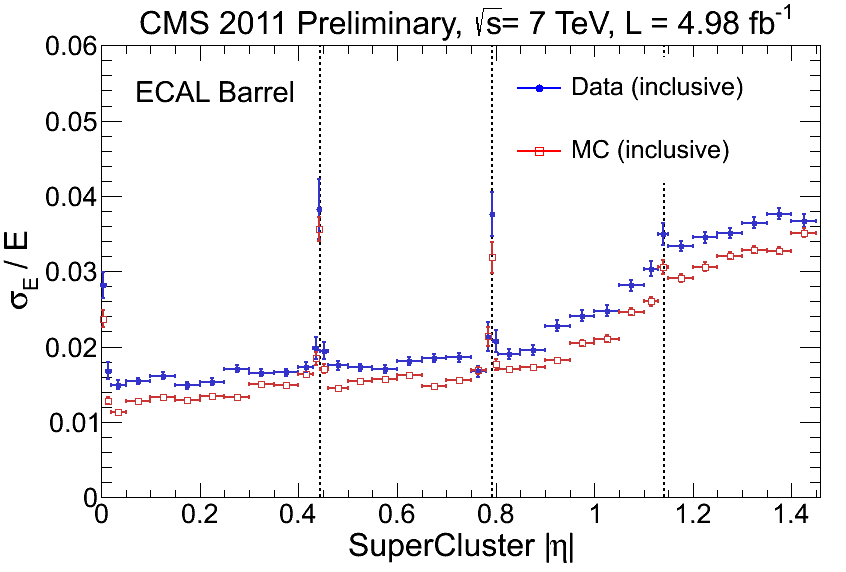
\includegraphics[scale=0.2]{ECAL_res_vs_eta_EB}}
	\hspace{1cm}
	\subfloat[EE \cite{ECAL_DPG_Twiki_res_vs_eta_EE}.]{\label{fig:ECAL_res_vs_eta_EE}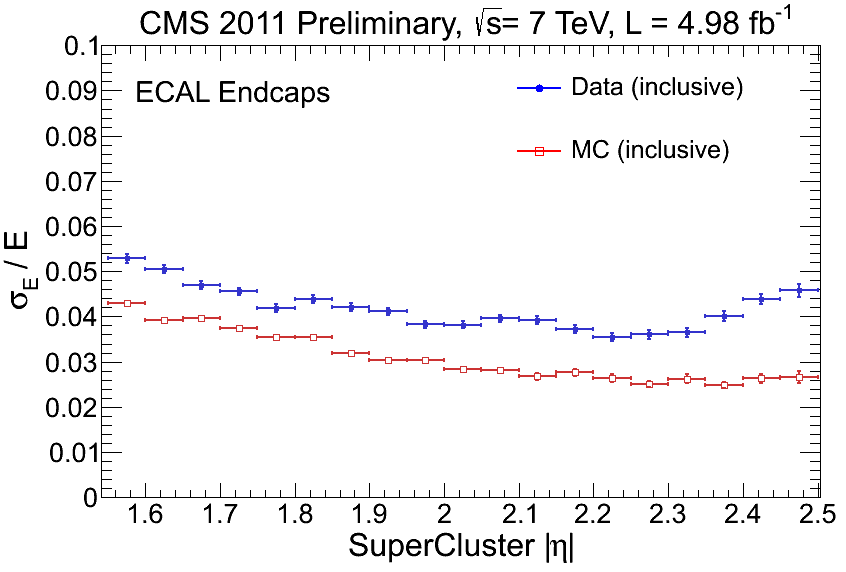
\includegraphics[scale=0.2]{ECAL_res_vs_eta_EE}}
	\caption{Energy resolution vs. $|\eta|$ for $Z$ decay electrons for data (filled blue circles) and MC (empty red squares).  The dotted lines show the locations of module gaps (three per SM).}
	\label{fig:ECAL_res_vs_eta}
\end{figure}

The 10-sample readout coupled with the fast scintillation time of lead tungstate allows for a very precise reconstruction of the time of ECAL hits.  ECAL timing is used for searches for long-lived particles that decay to photons or jets, such as long-lived neutralinos in GMSB \cite{CMS-PAS-EXO-11-067}.  Figure~\ref{fig:ECAL_timing_res} shows the timing resolution in EE.

\begin{figure}
	\centering
	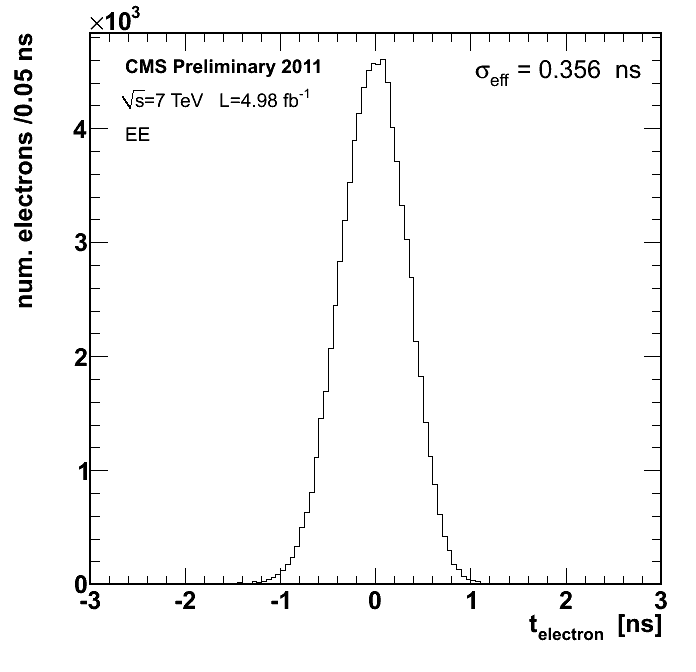
\includegraphics[scale=0.3]{ECAL_timing_res}
	\caption{Distribution of reconstructed times of $Z$ decay electrons in EE \cite{ECAL_DPG_Twiki_timing_res}.}
	\label{fig:ECAL_timing_res}
\end{figure}

\subsection{Hadronic Calorimeter}

The CMS hadronic calorimeter (HCAL) has four parts: HCAL barrel (HB), HCAL endcap (HE), and HCAL outer (HO), which all utilize the same brass absorber / plastic scintillator sandwich technology; and HCAL forward (HF), which is a \u{C}erenkov detector made of quartz fibers.  A quarter longitudinal cross-sectional view of HCAL is shown in Figure~\ref{fig:HCAL_longitudinal_xsec}.  Like EB, HB is formed of 36 $\phi$-wedges (18 cover $2\pi$ in positive $\eta$, 18 cover $2\pi$ in negative $\eta$).  Each wedge is divided into 16 along $\eta$ and four along $\phi$, for a total of 64 readout towers per wedge (compare 1700 individually read out crystals per EB wedge).  HE is divided into 36 $\phi$-wedges containing 38 readout towers each.  HO consists of five rings around HB and HE distributed symmetrically along $z$.  There are 72 $\phi$-slices per ring, with each $\phi$-slice further divided into 5, 6, or 8 along $z$ depending on ring.  The HF fibers are distributed within the steel absorber.  HF is divided into 18 $\phi$-wedges per endcap side, each containing 24 readout towers.  All HB towers have a single readout channel except for the two in each wedge at highest $|\eta|$, which are segmented into two longitudinal layers for readout.  In HE, all towers have two longitudinal readout layers, except for the three rings of towers closest to the beam line, which have three.  There are also two longitudinal depths of HF fibers.

\begin{figure}
	\centering
	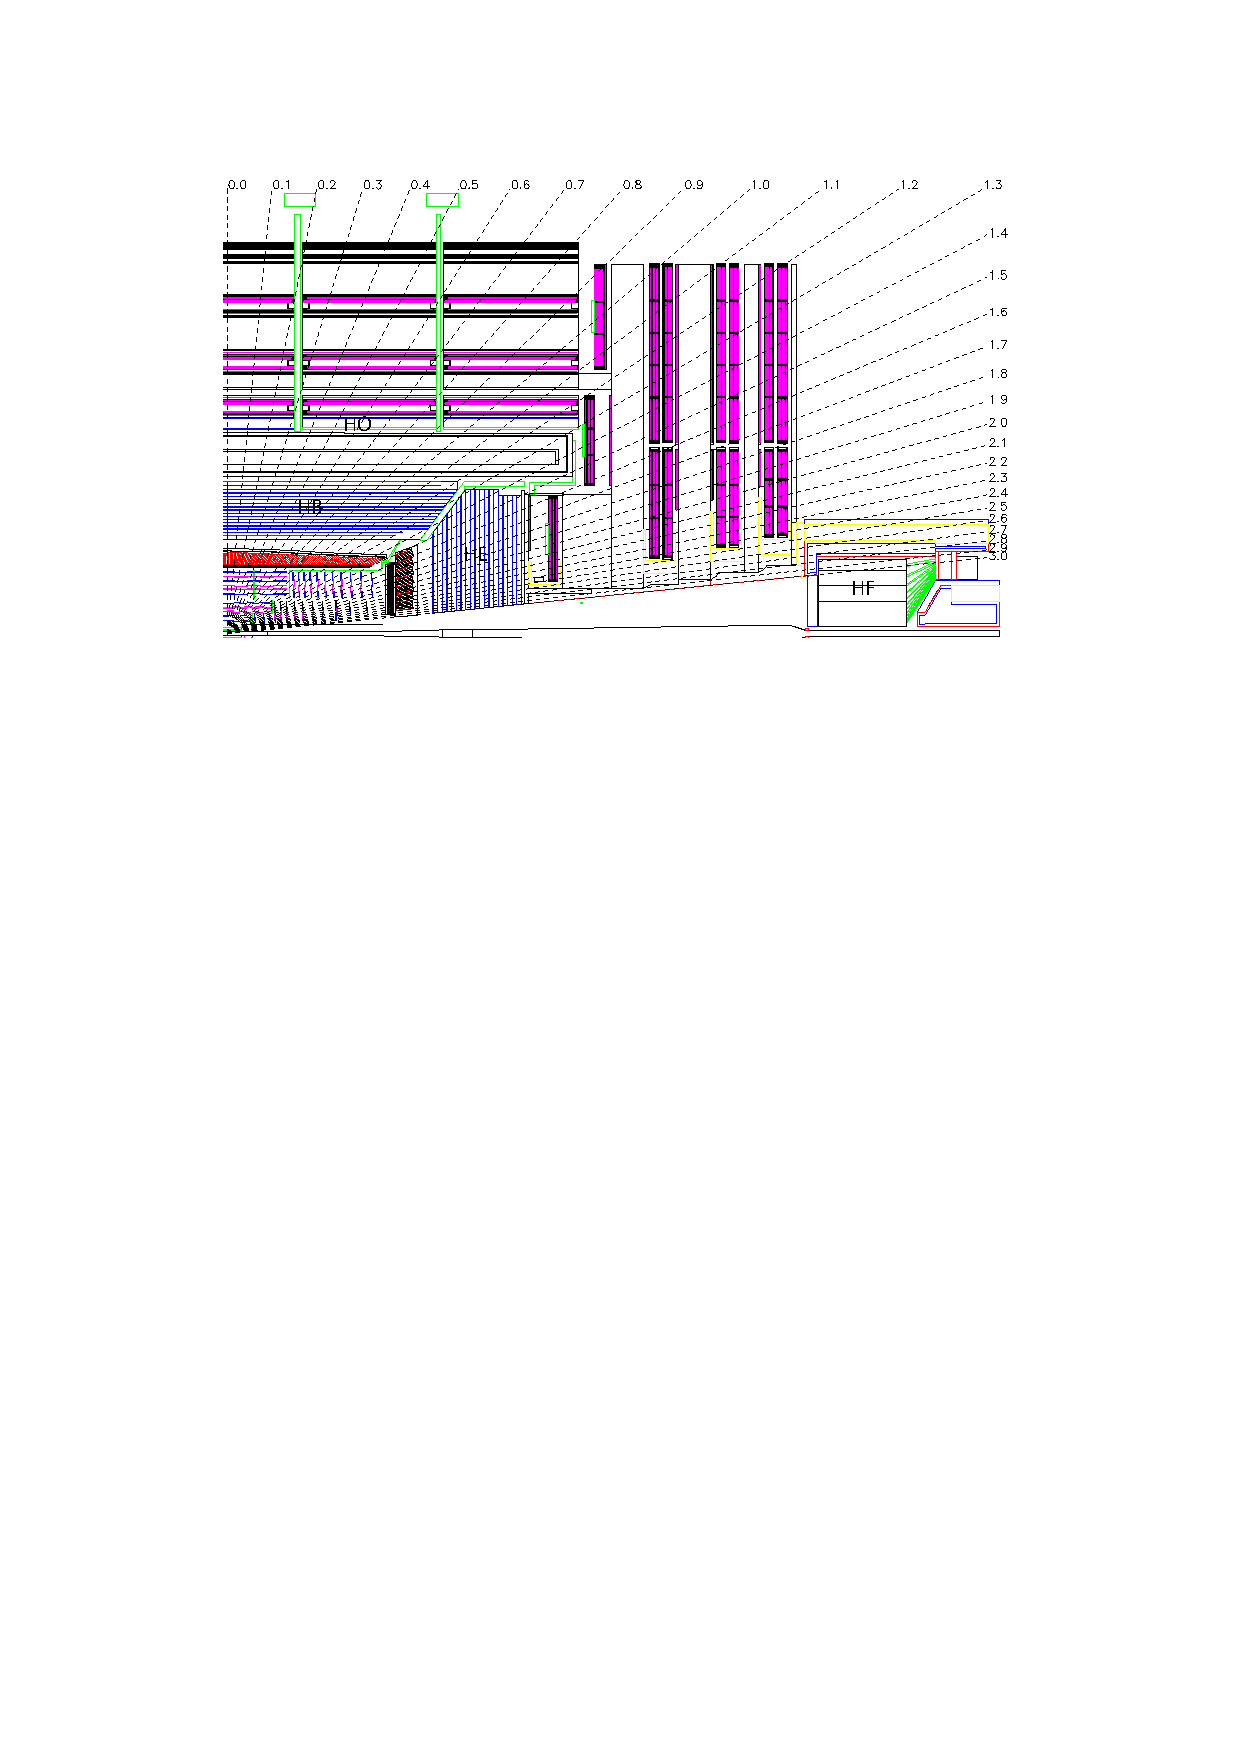
\includegraphics[scale=1.0]{HCAL_longitudinal_xsec}
	\caption{Quarter longitudinal cross-sectional view of HCAL (and muon stations in purple).  Reprinted from Fig. 5.1 of ref. \cite{1748-0221-3-08-S08004}.}
	\label{fig:HCAL_longitudinal_xsec}
\end{figure}

HB, HE, and HO are all sampling calorimeters consisting of alternating layers of brass absorber and plastic scintillator.  The absorber initiates the hadronic shower, and as shower particles travel through the scintillator the scintillation light is read out by wavelength-shifting (WLS) fibers connected to the scintillator tiles.\footnote{By contrast, in the ECAL, the crystal material acts as both absorber and scintillator, greatly reducing the contribution to energy resolution from sampling fluctuations.}  The full development of the shower is sampled by the layers of instrumented scintillator.  The scintillator tiles are staggered so that there are no cracks in coverage along the direction projected back to the beam spot.  Light output from all tiles in a single readout tower is collected via the WLS fibers and merged into a single signal that is amplified by a hybrid photodiode (HPD).  A diagram of the optical readout of HB (similar for HE and HO) is shown in Figure~\ref{fig:HCAL_HB_optics}.

\begin{figure}
	\centering
	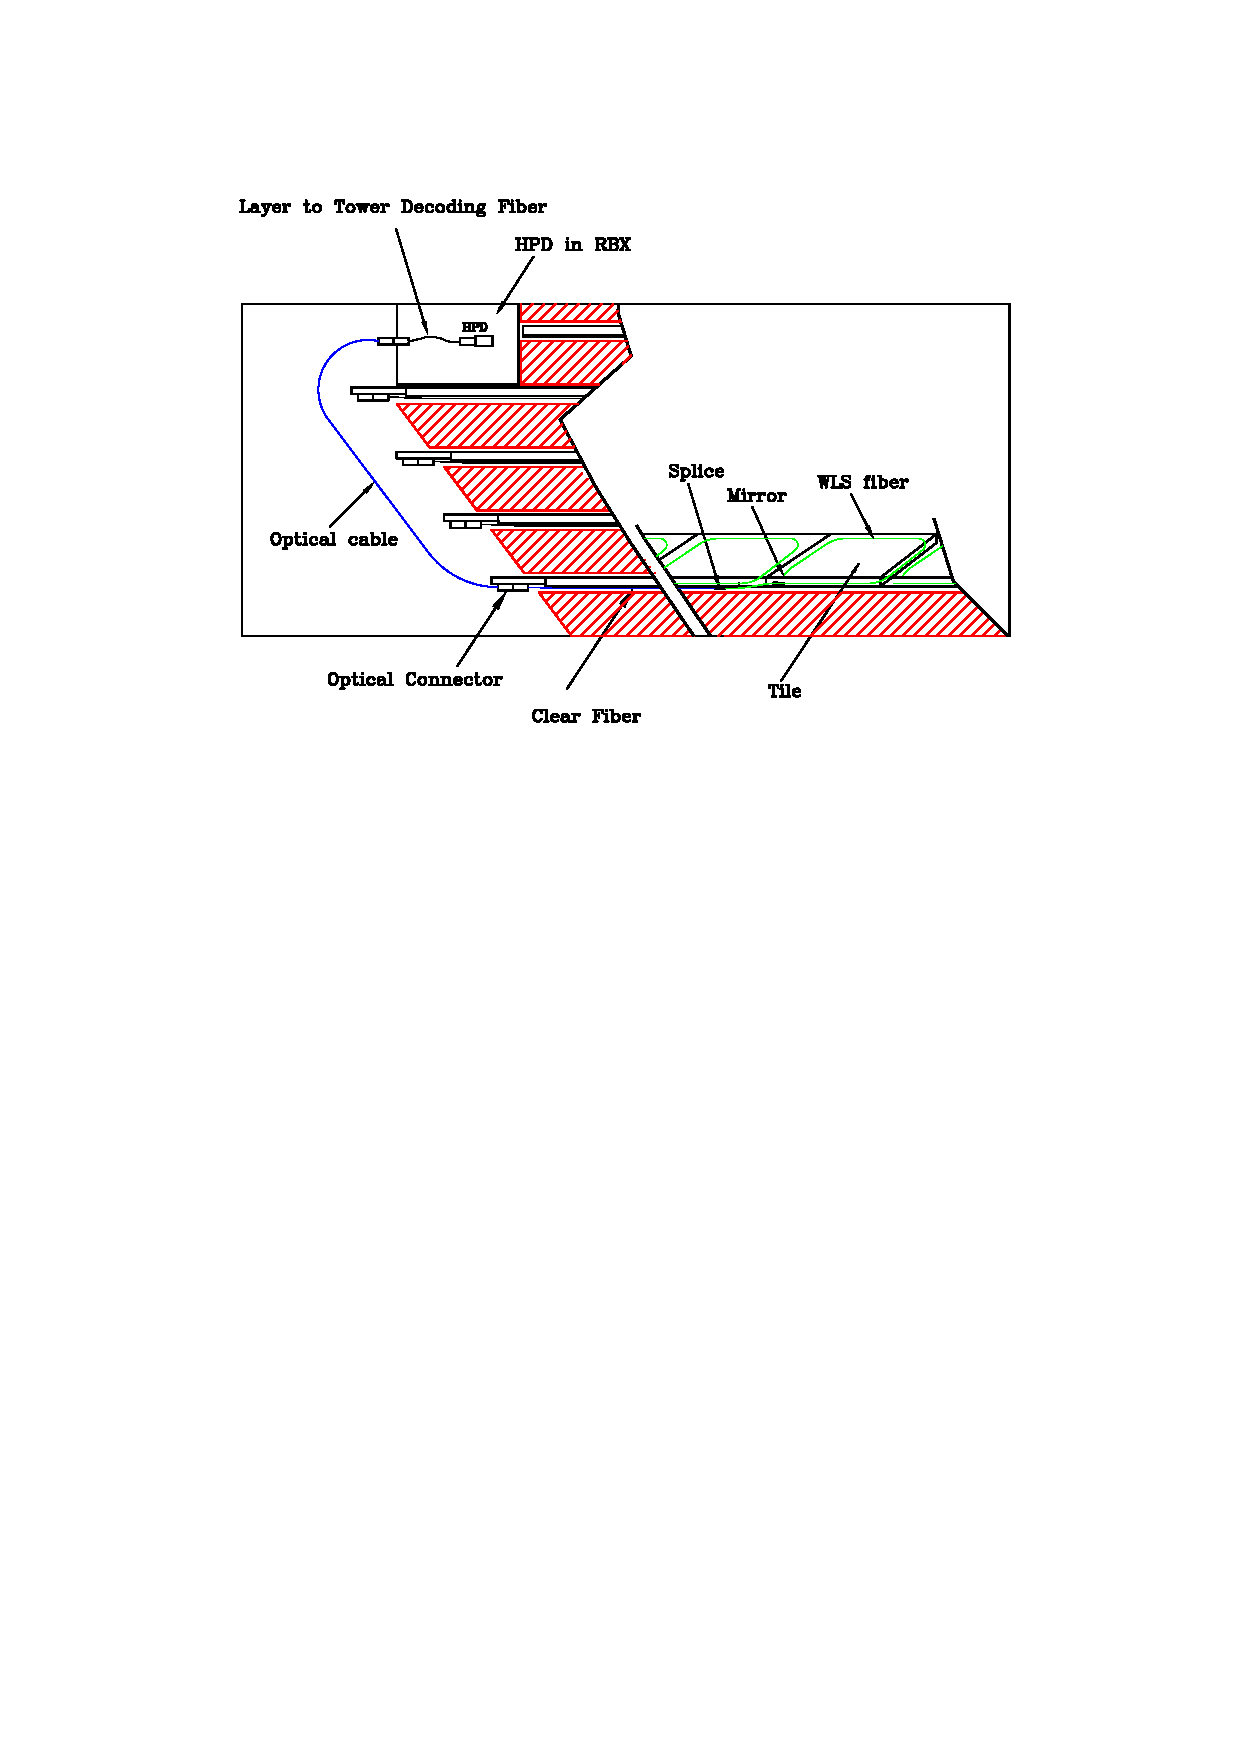
\includegraphics[scale=1.0]{HCAL_HB_optics}
	\caption{Diagram of the optical readout of HB.  Reprinted from Fig. 5.7 of ref. \cite{1748-0221-3-08-S08004}.}
	\label{fig:HCAL_HB_optics}
\end{figure}

Due to the extremely harsh radiation environment near the beam line, HF is constructed of a 1.2-m thick, 1.7-m long ring of steel absorber with radiation hard quartz fibers distributed within the steel and running parallel to the beam line.  Hadronic showers develop in the steel and are sampled in the quartz fibers when charged shower particles hit the the fibers and emit \u{C}erenkov light.  The light is transmitted by total internal reflection down the fibers to a photomultiplier tube (PMT), where the signals from all fibers in an HF tower are merged into one.  Since only relativistic particles emit \u{C}erenkov light in these fibers, it is mostly the EM component of the hadronic shower, consisting of neutral pions decaying to photons that interact electromagnetically with the absorber, that is sampled \cite{Akchurin_Wigmans}.  The charged hadrons produced in hadronic showers are typically too slow to generate \u{C}erenkov light.  Figure~\ref{fig:HCAL_HF_xsec} shows a cross-sectional view of one side of HF.

\begin{figure}
	\centering
	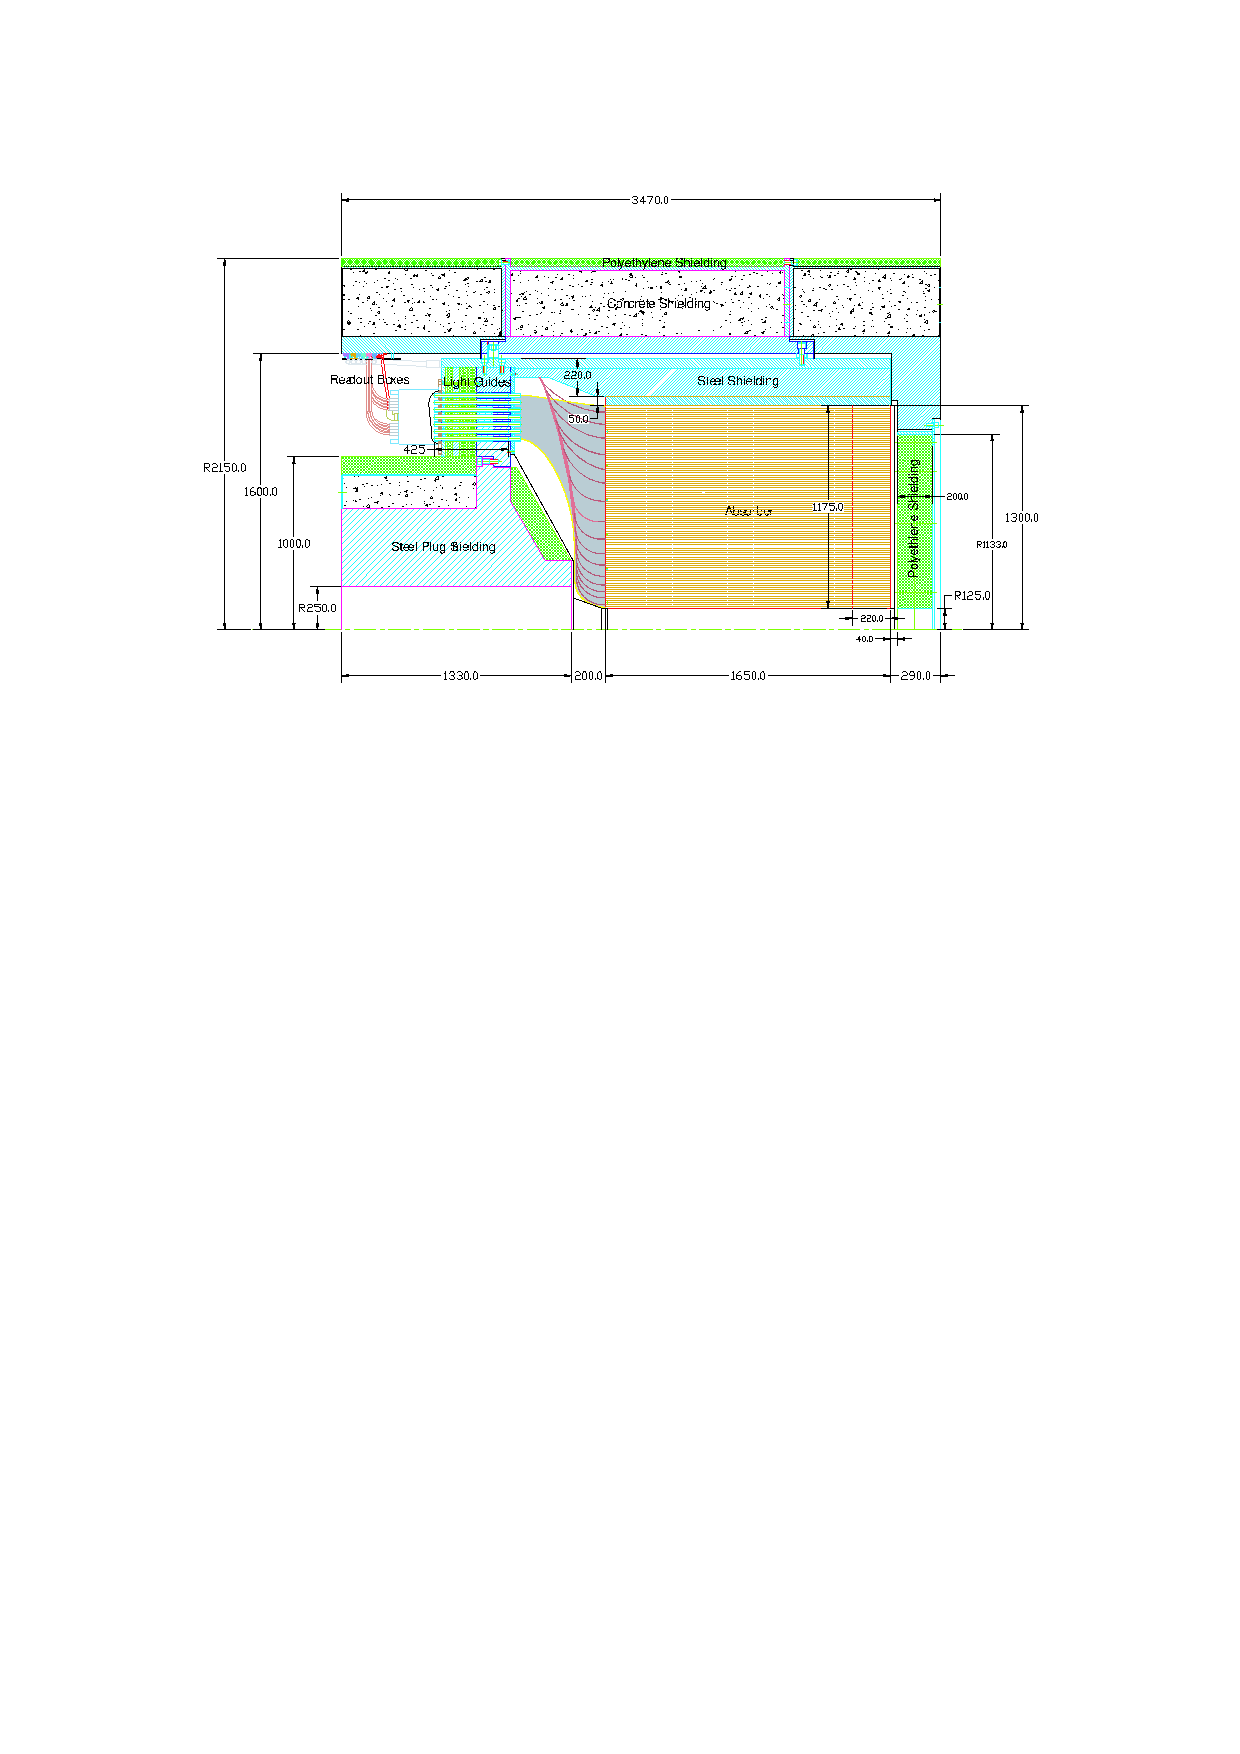
\includegraphics[scale=1.0]{HCAL_HF_xsec}
	\caption{Cross-sectional view of one side of HF.  The $z$-axis is horizontal.  Reprinted from Fig. 5.28 of ref. \cite{1748-0221-3-08-S08004}.}
	\label{fig:HCAL_HF_xsec}
\end{figure}

Electrical signals from either HPDs (HB/HE/HO) or PMTs (HF) are digitized on the front ends by means of a fast charge-integrating ADC.  The digitized signals are sent off-detector to the HCAL Trigger/Read-Out (HTR) boards, where they await a trigger decision.  If the trigger is accepted, the signals are sent on to the HCAL data concentrator cards (DCCs), which interface to the global DAQ system.  HCAL trigger primitives, consisting of transverse energy sums over an entire tower, are calculated in the HTR boards and sent to the global trigger system.

Selected HCAL performance results can be seen in Figure~\ref{fig:HCAL_performance}.

\begin{figure}
	\centering
 	\subfloat[Data/MC comparison of HB response to charged tracks of 9-11 GeV/$c$ momentum \cite{CMS-DP-2010-025}.]{\label{fig:HCAL_performance_HB_response}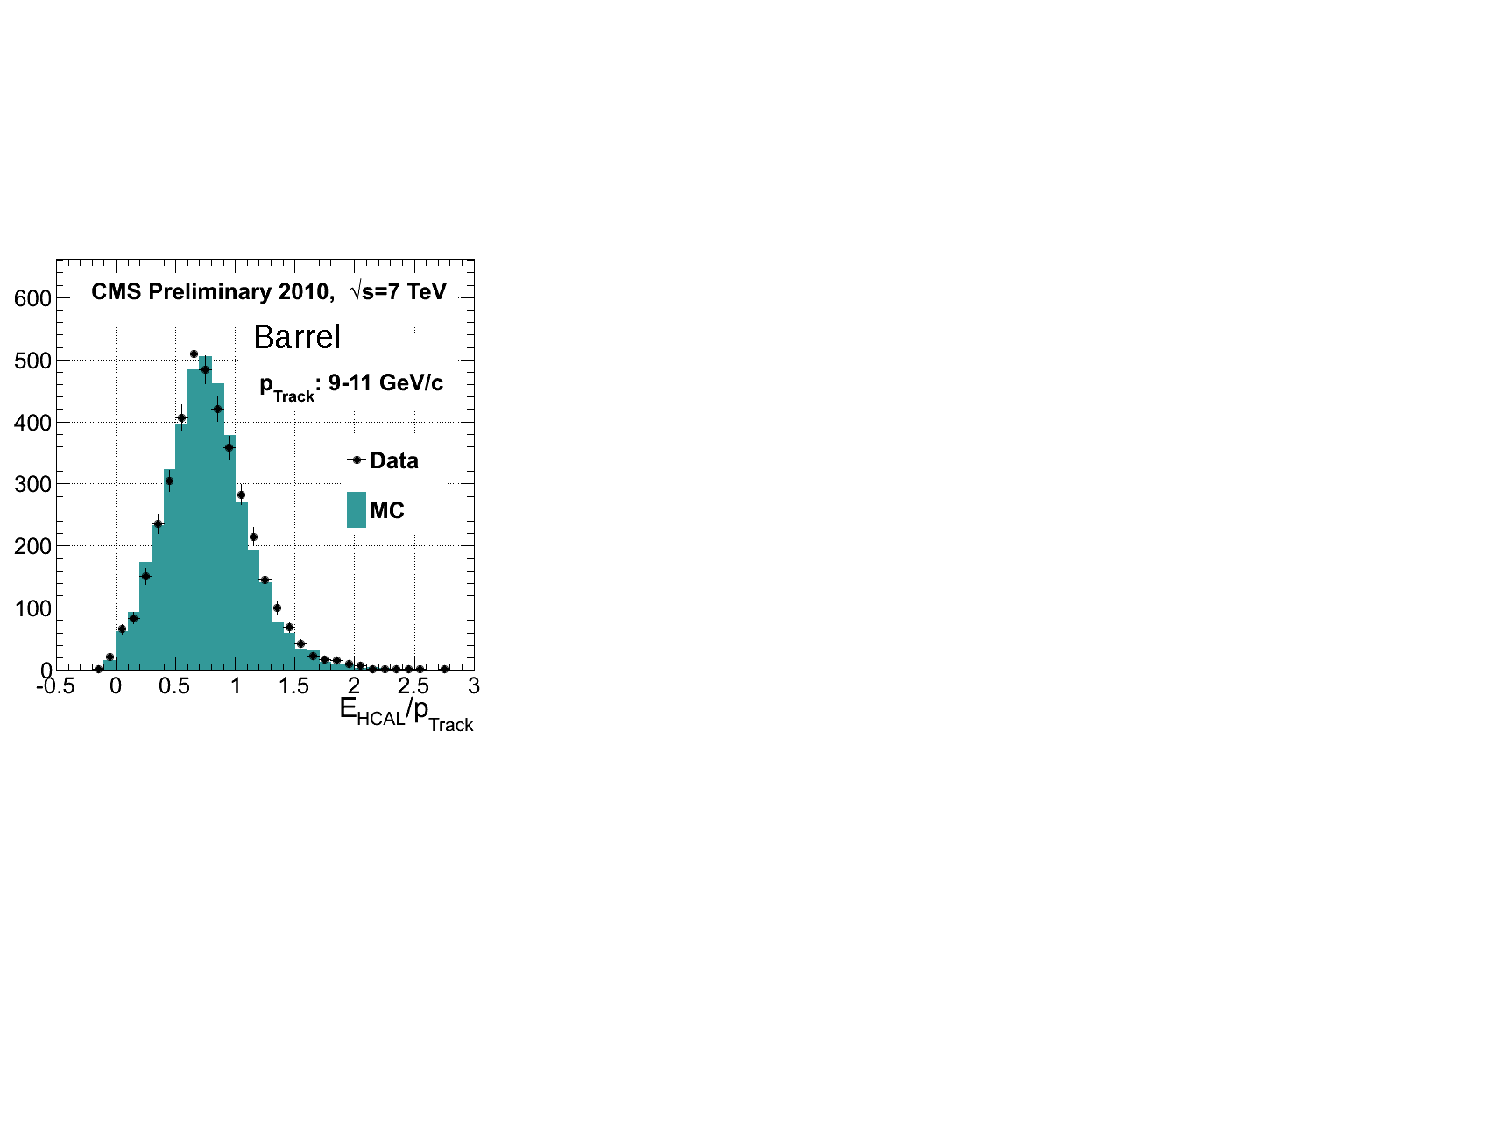
\includegraphics[scale=0.7]{HCAL_performance_HB_response}}
	\\
	\subfloat[Distribution of tower multiplicity, clearly showing three peaks in rate corresponding to noise sources (see Sec.~\ref{sec:Event Quality}) \cite{1748-0221-5-03-T03014}.]{\label{fig:HCAL_performance_noise}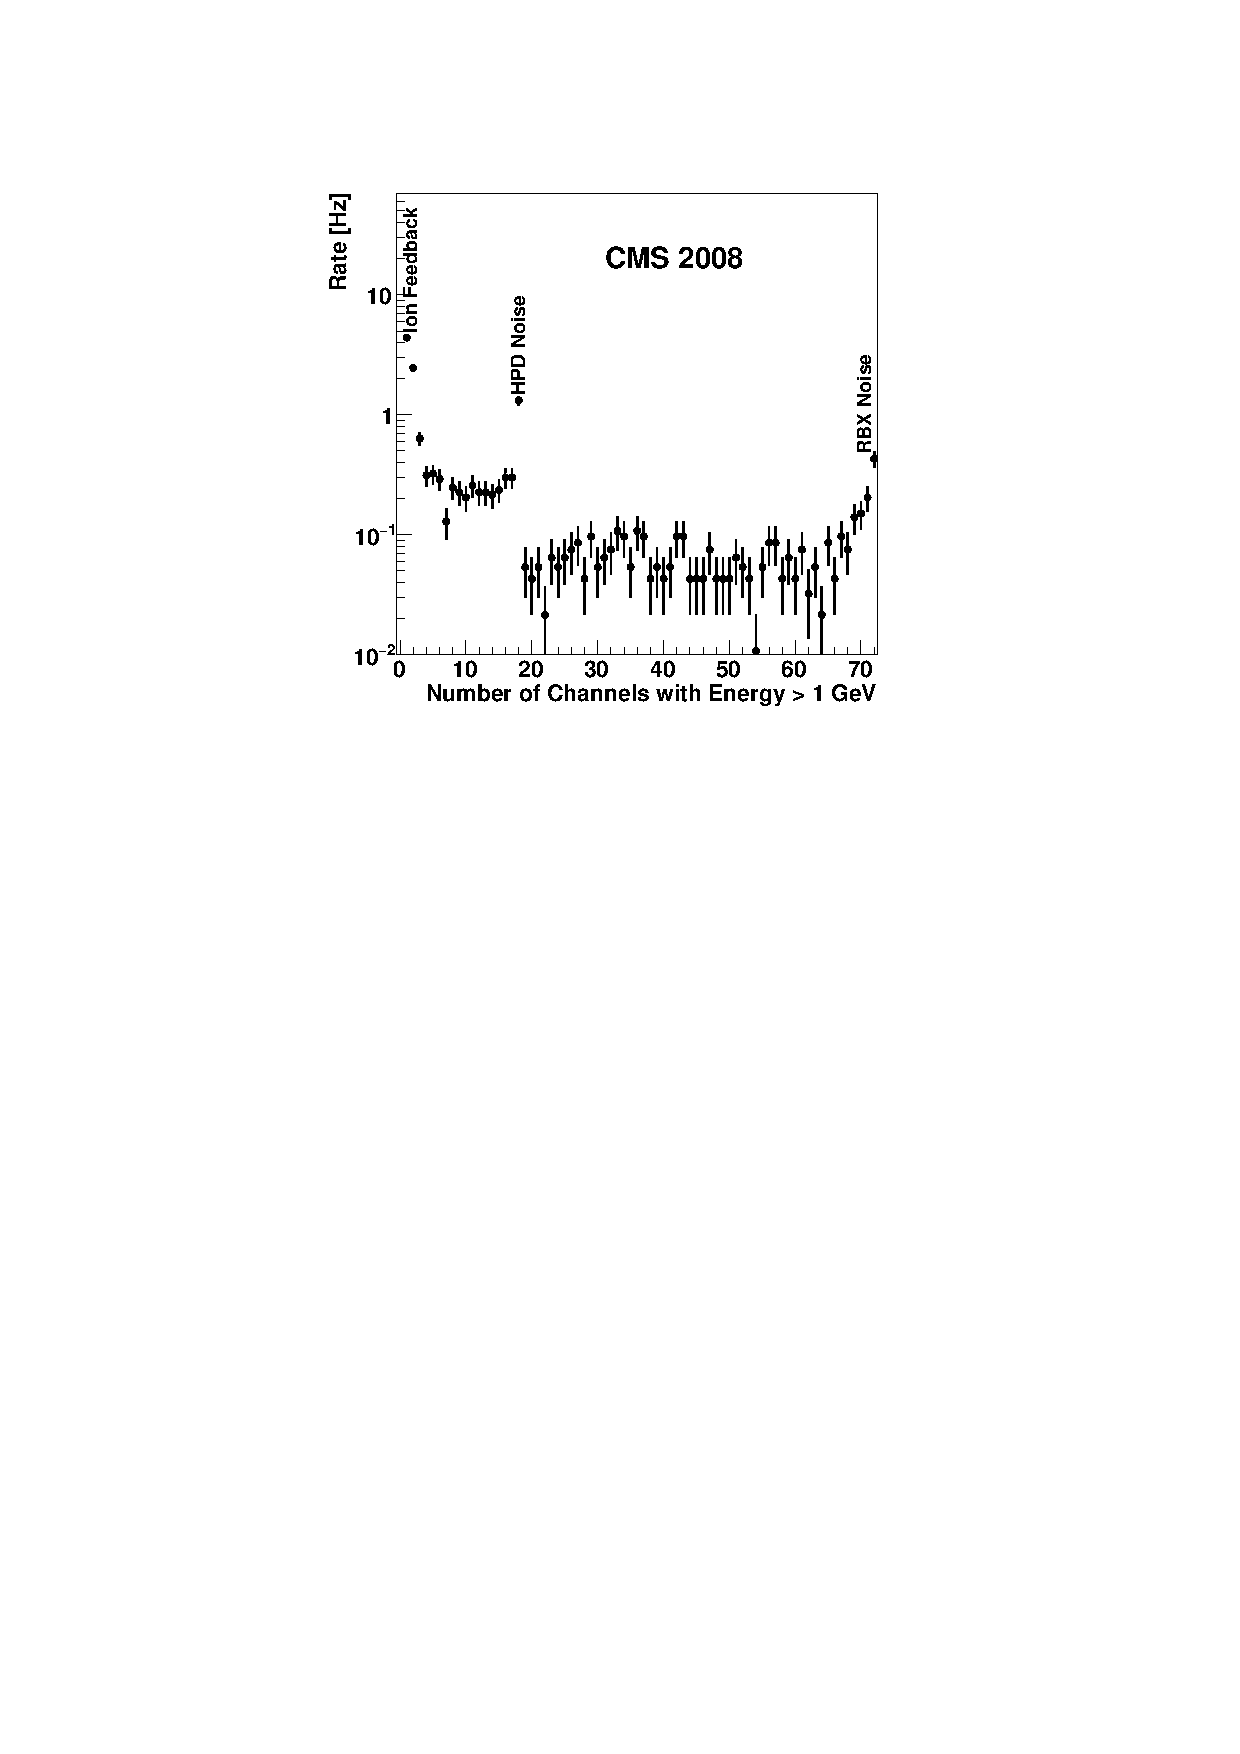
\includegraphics[scale=0.7]{HCAL_performance_noise}}
	\\
	\subfloat[Timing resolution vs. tower energy \cite{CMS-DP-2010-025}.]{\label{fig:HCAL_performance_timing}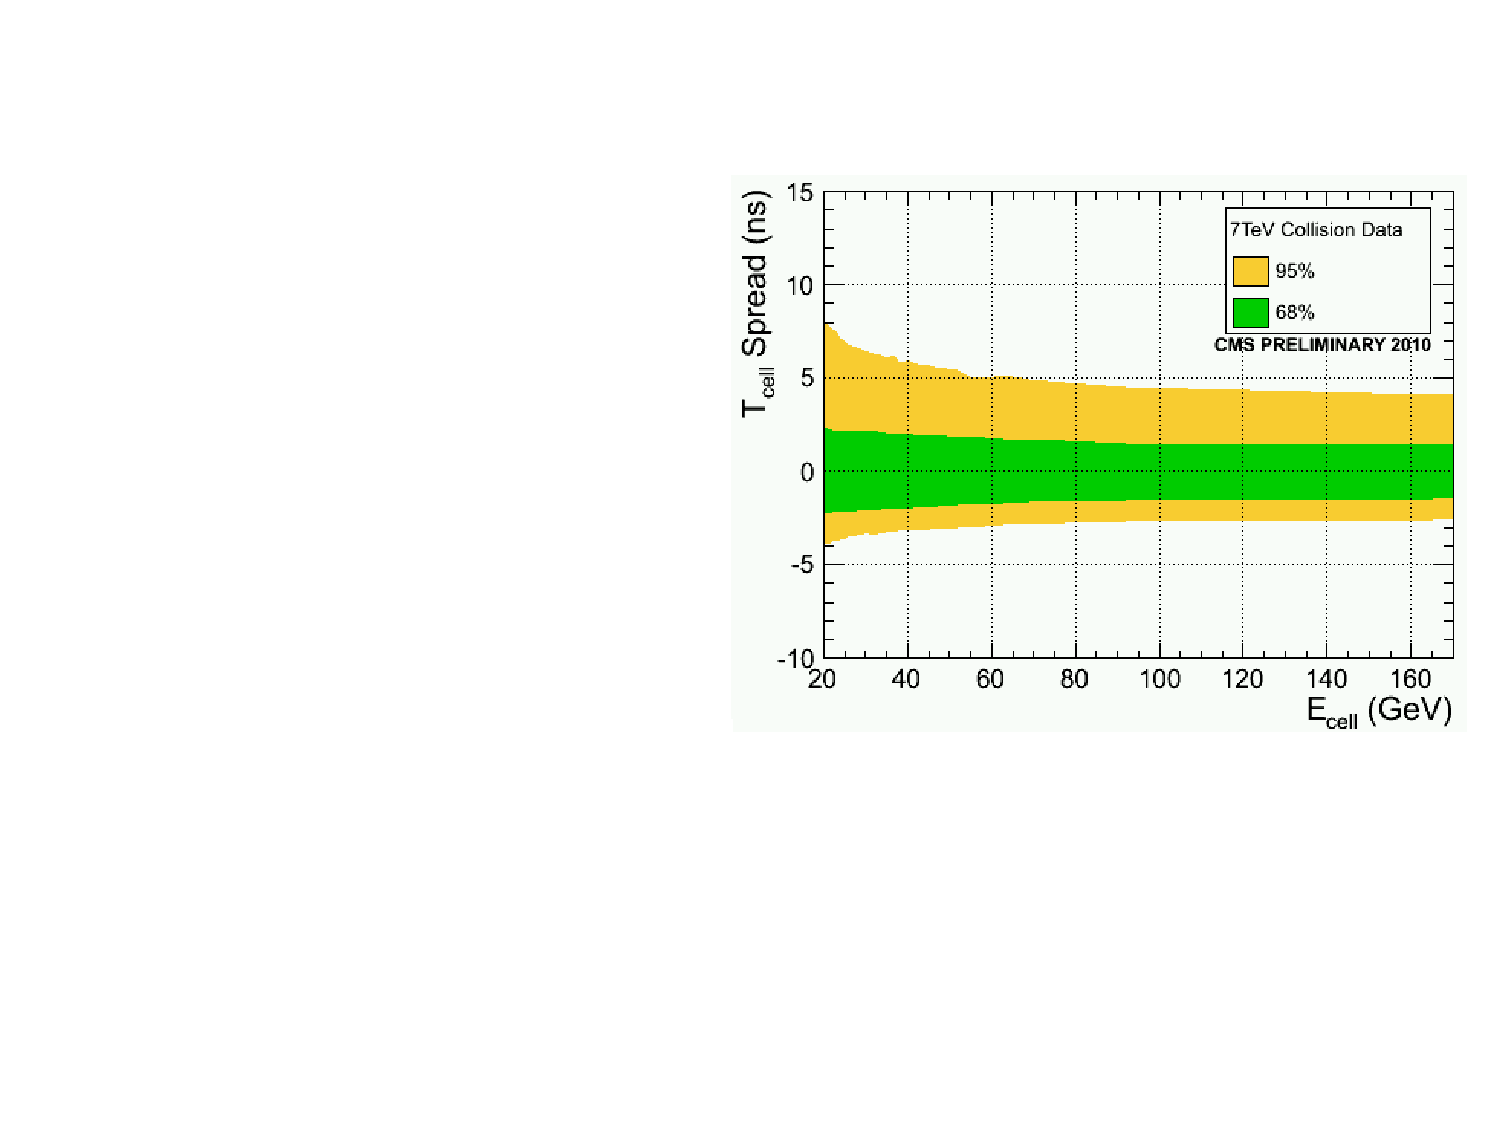
\includegraphics[scale=0.7]{HCAL_performance_timing}}
	\caption{Selected HCAL performance results.}
	\label{fig:HCAL_performance}
\end{figure}

\subsection{Muon System}

Beginning at a radius of $\sim10$ interaction lengths from the beam line, where all particles except muons should have been stopped by the HCAL, are the muon chambers, interspersed with the iron return yoke of the CMS magnetic field.  Three technologies are employed: drift tubes in the barrel section (MB), cathode strip chambers (CSCs) in the endcap section (ME), and resistive plate chambers (RPCs) in both sections to provide an independent trigger with superior time resolution.  There are four barrel layers of stations extending out to $|\eta| = 1.2$.  Each endcap consists of five disks of stations as shown in Figure~\subref*{fig:muons_layout_ME}, covering $1.4 < |\eta| < 2.4$.  RPCs populate the barrel and endcap muon systems alongside the DT chambers and CSCs.  Since they have time resolution much better than a few ns, they are used to assign the bunch crossing of muon tracks and provide a $p_{T}$ trigger with sharp turn-on.

\begin{figure}
	\centering
 	\subfloat[One of the five wheels of MB, showing the four layers of muon stations.  The five wheels are spaced symmetrically in $z$ about $z = 0$.  As a muon traverses the muon detectors, its curvature in the transverse plane changes direction and magnitude due to the magnetic field in the return yoke, which is of opposite sign and reduced strength relative to the field within the solenoid volume.  Reprinted from Fig. 7.3 of ref. \cite{1748-0221-3-08-S08004}.]{\label{fig:muons_layout_MB}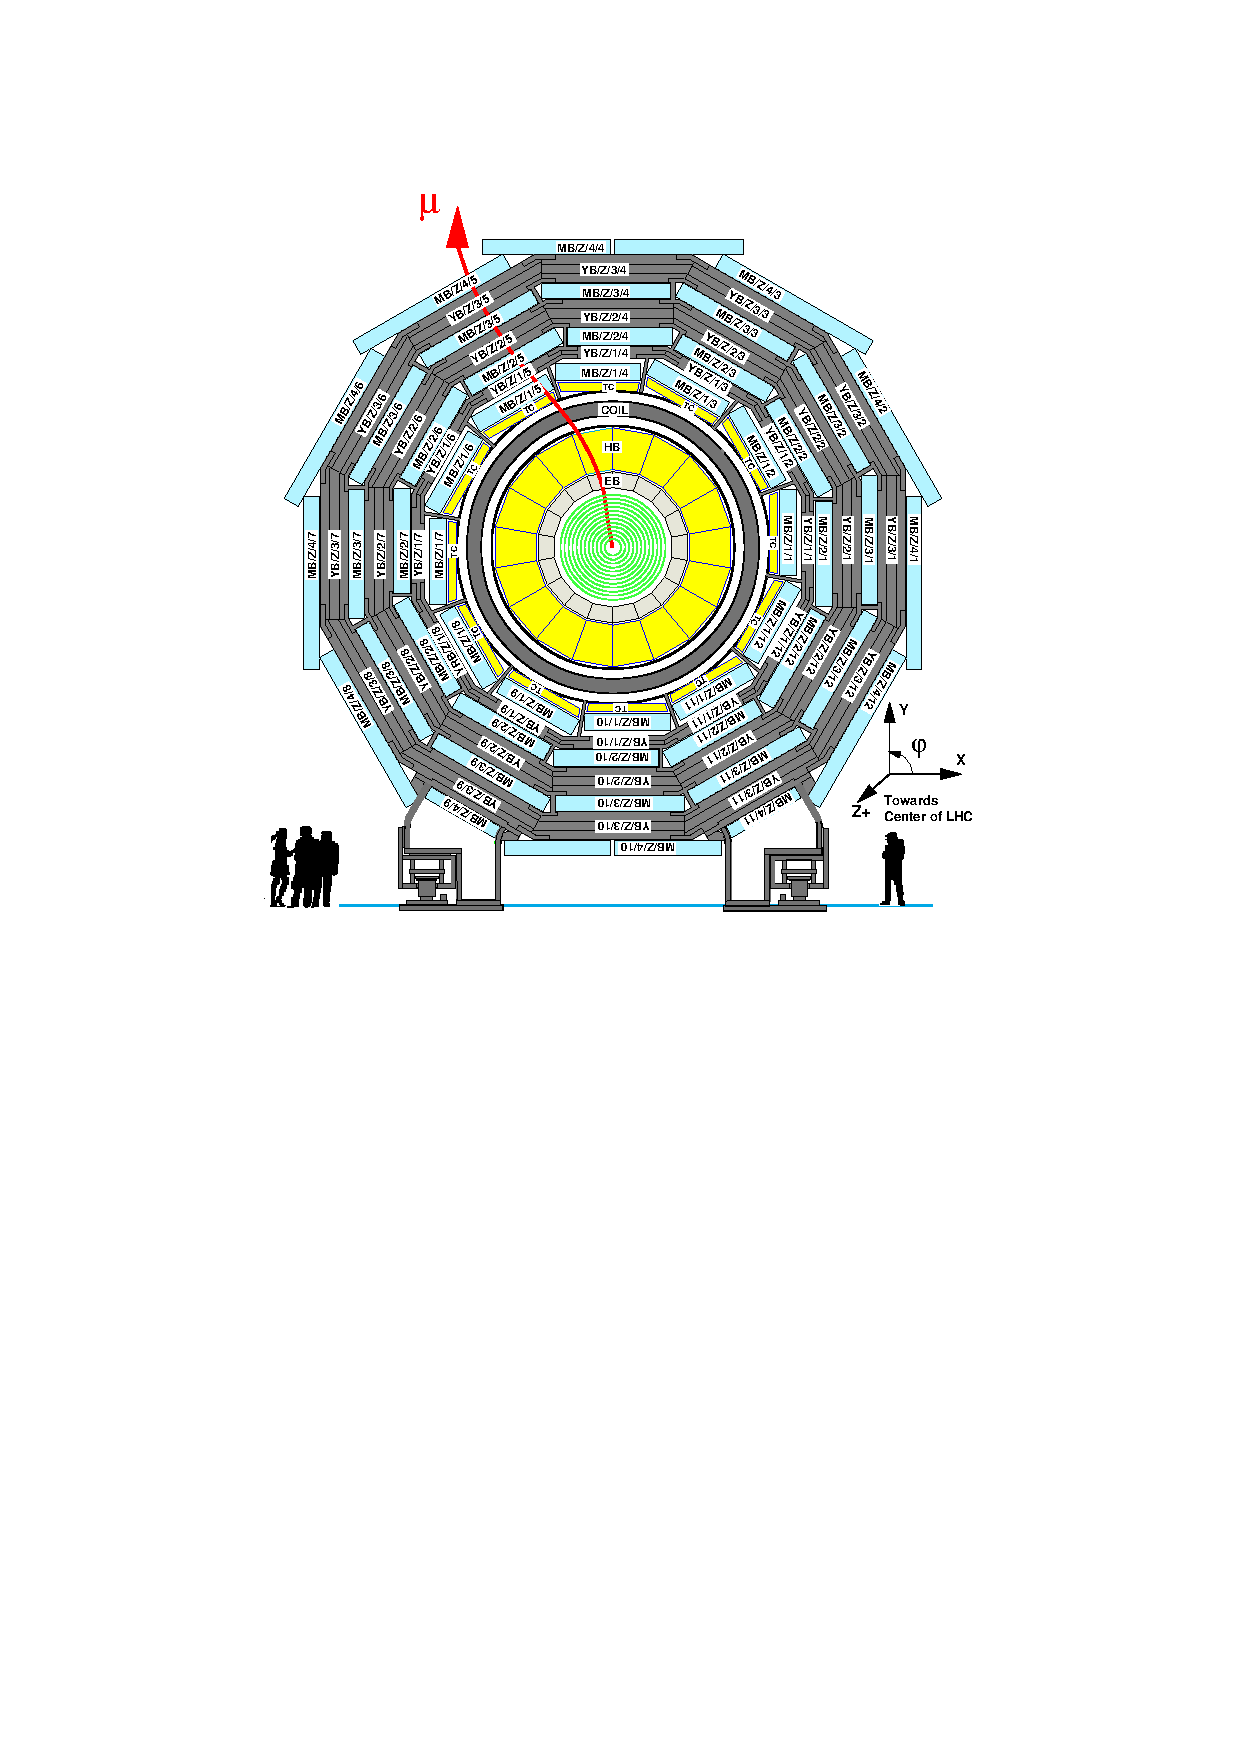
\includegraphics[scale=0.6]{muons_layout_MB}}
	\\
	\subfloat[Quarter longitudinal cross section of CMS highlighting the location of the ME disks.  Reprinted from Fig. 7.47 of ref. \cite{1748-0221-3-08-S08004}.]{\label{fig:muons_layout_ME}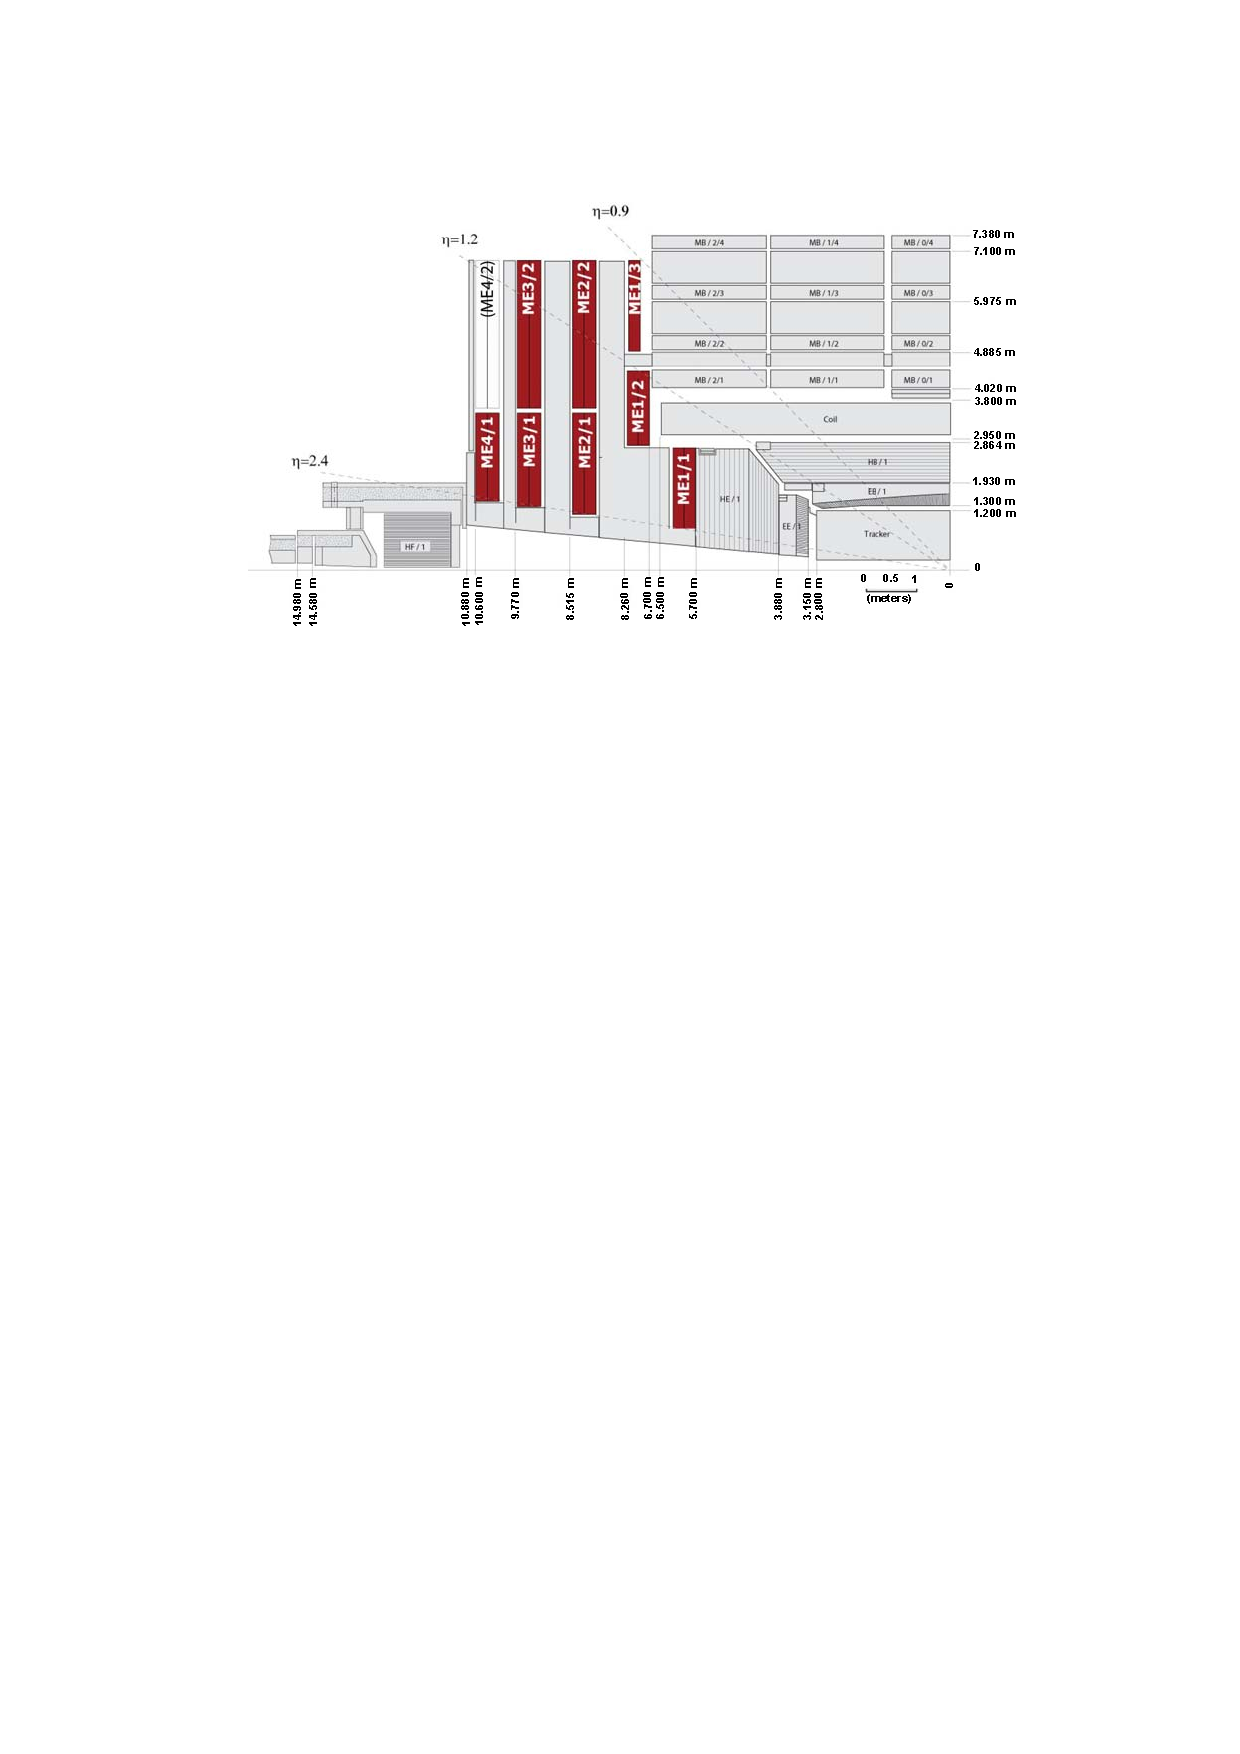
\includegraphics[scale=0.6]{muons_layout_ME}}
	\caption{View of the MB and ME layout in CMS.}
	\label{fig:muons_layout}
\end{figure}

Each DT chamber consists of two $r\cdot\phi$ superlayers (SLs) and optionally one $z$ SL (in all chambers except those in the fourth layer).  The SLs contain four rows of drift tubes, with the rows staggered such that there are no gaps in the coverage.  The $r\cdot\phi$ SLs have the tube axis parallel to the beam line, while the $z$ SL is perpendicular to the beam line.  The tubes are $\sim2.4$ m in length and $13\mbox{ mm}\times42\mbox{ mm}$ in cross section.  Each chamber therefore records eight $r\cdot\phi$ tracking points and optionally four $z$ tracking points.  The tubes are filled with an 85\%Ar + 15\% $\mbox{CO}_{2}$ gas mixture.  An anode wire at 3600 V runs the length of the tube, while the walls are covered with electrodes held at 1800 V or -1200 V depending on wall.  When a muon passes through the tube, it ionizes the gas atoms.  The liberated electrons drift along the electric field lines created by the electrodes to the anode, which is read out.  Figure ~\ref{fig:muons_DT} shows the electric field lines within a drift tube as well as the contours of equal drift time.  The maximum drift time is 380 ns.

\begin{figure}
	\centering
	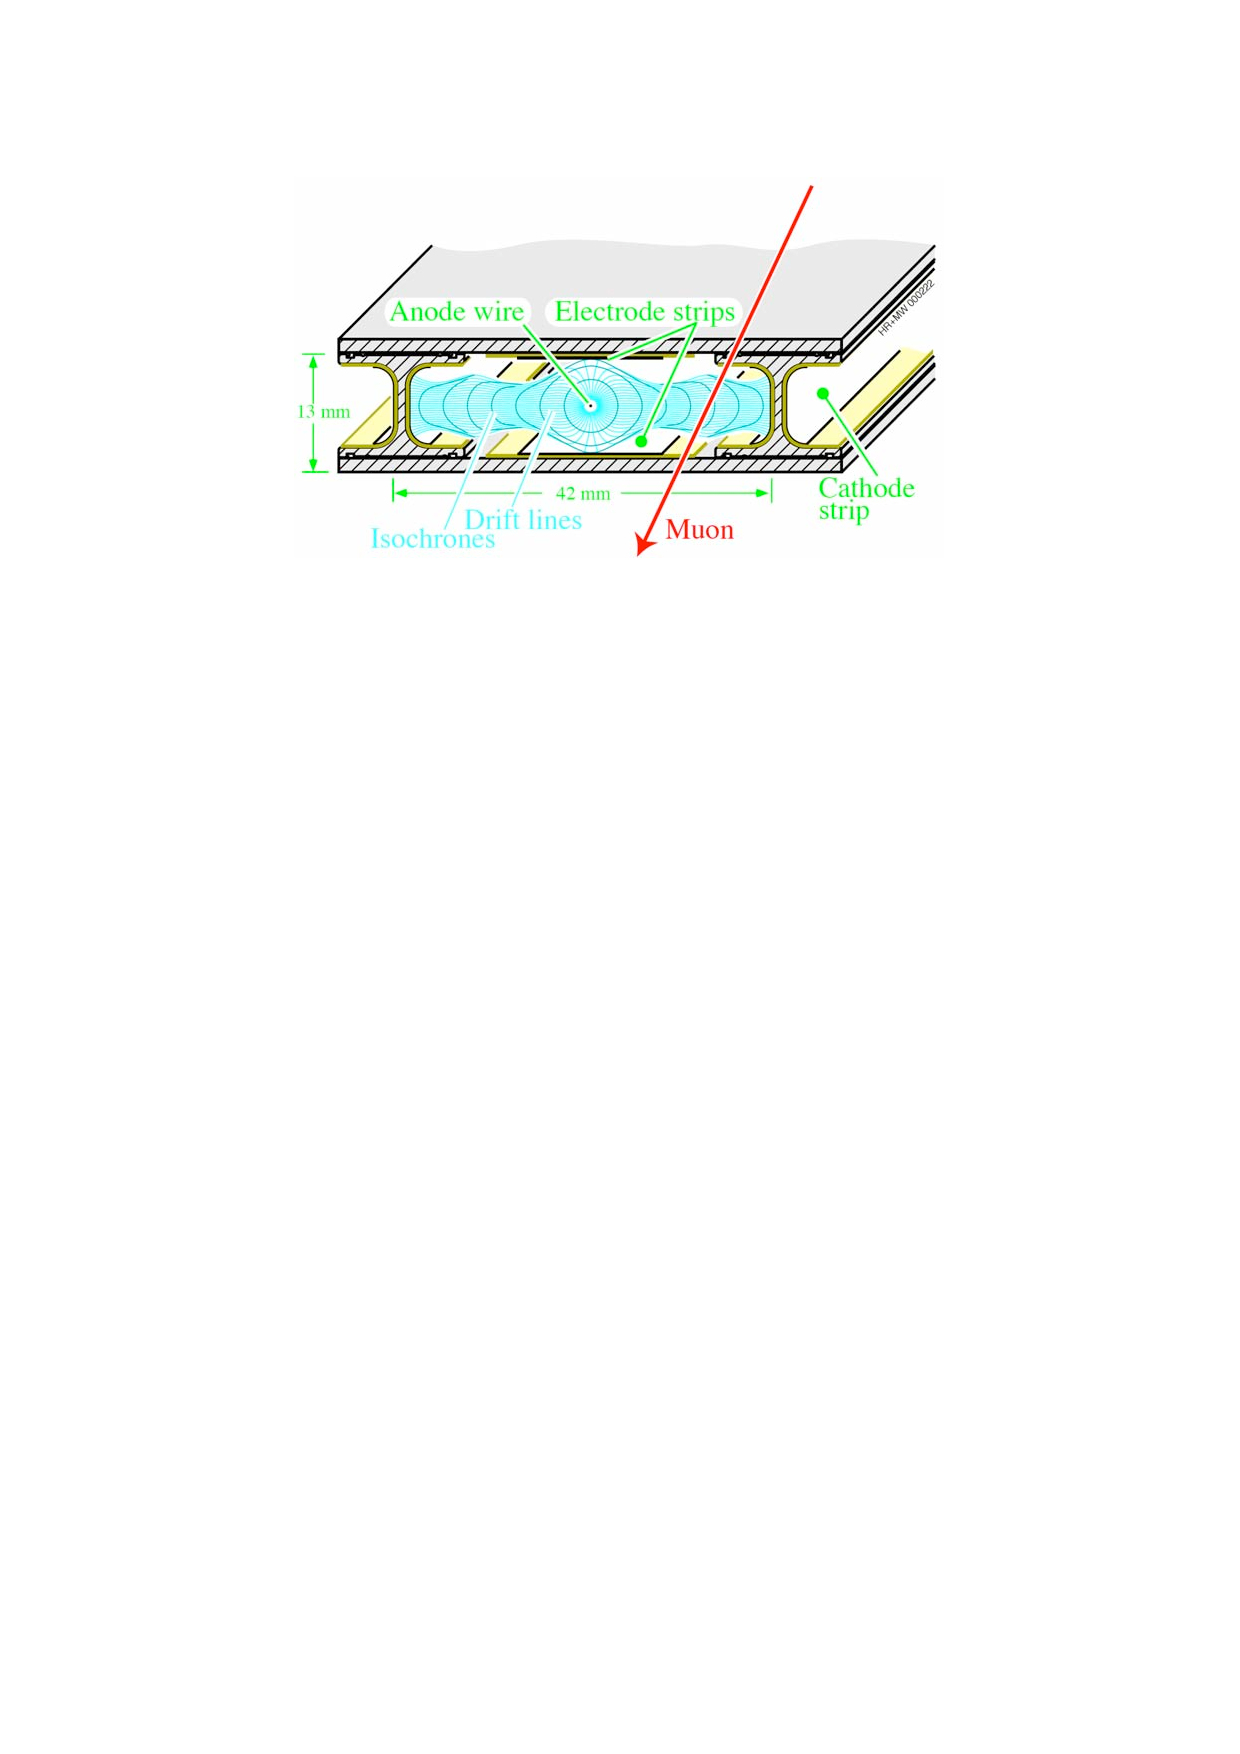
\includegraphics[scale=1.0]{muons_DT}
	\caption{Electric field lines within a drift tube as well as the contours of equal drift time.  Reprinted from Fig. 7.5 of ref. \cite{1748-0221-3-08-S08004}.}
	\label{fig:muons_DT}
\end{figure}

CSCs consist of alternating layers of cathode strips (four planes oriented along $r$) and anode wires (three planes oriented along $\phi$).  A 40\%Ar + 50\%$\mbox{CO}_{2}$ + 10\%$\mbox{CF}_{4}$ gas mixture fills the space between two successive planes, forming six gas gaps.  When a muon ionizes the gas atoms, the positive ions drift toward the anode and are read out to provide a measurement of $r$, just as in the DTs.  However, an image charge is induced on the cathode strips, which is also read out to provide a measurement of $\phi$.  The wires are spaces 3.2 mm apart.  The cathode strips have pitch varying from 8.4 mm at the end closest to the beam line to 16 mm at the other end, and are spaced 0.5 mm apart.  A trapezoidal CSC is shown in Figure~\ref{fig:muons_CSC_wedge}.

\begin{figure}
	\centering
	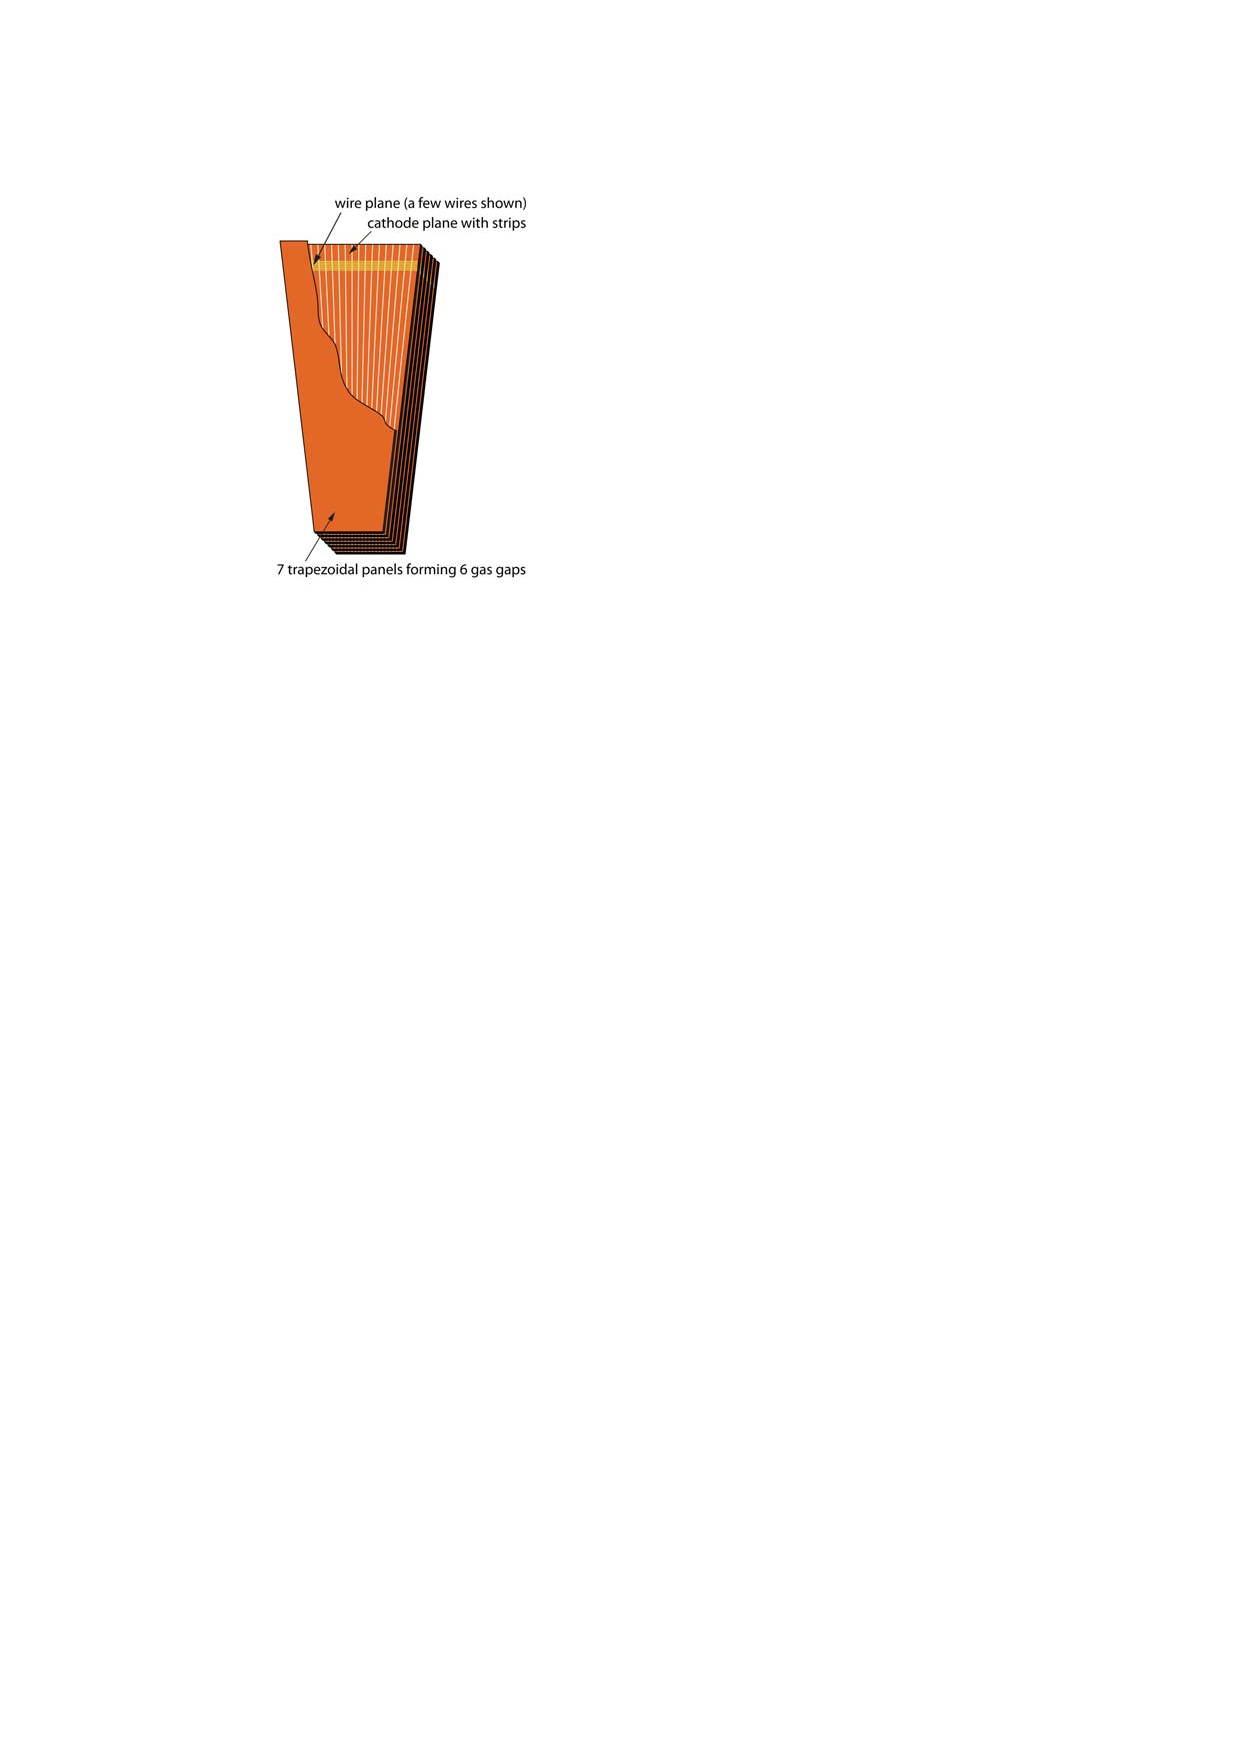
\includegraphics[scale=1.0]{muons_CSC_wedge}
	\caption{CSC wedge, showing the cathode and wire planes.  Reprinted from Fig. 7.49 of ref. \cite{1748-0221-3-08-S08004}.}
	\label{fig:muons_CSC_wedge}
\end{figure}

Track stubs from the muon system are combined with tracks from the tracking system to form more precise muon tracks than either system could form alone, as shown in Figure~\ref{fig:muon_pT_res}.  This leads to extremely good di-muon invariant mass resolution (Figure~\ref{fig:muon_inv_mass}) over a large $p_{T}$ range.

\begin{figure}
	\centering
	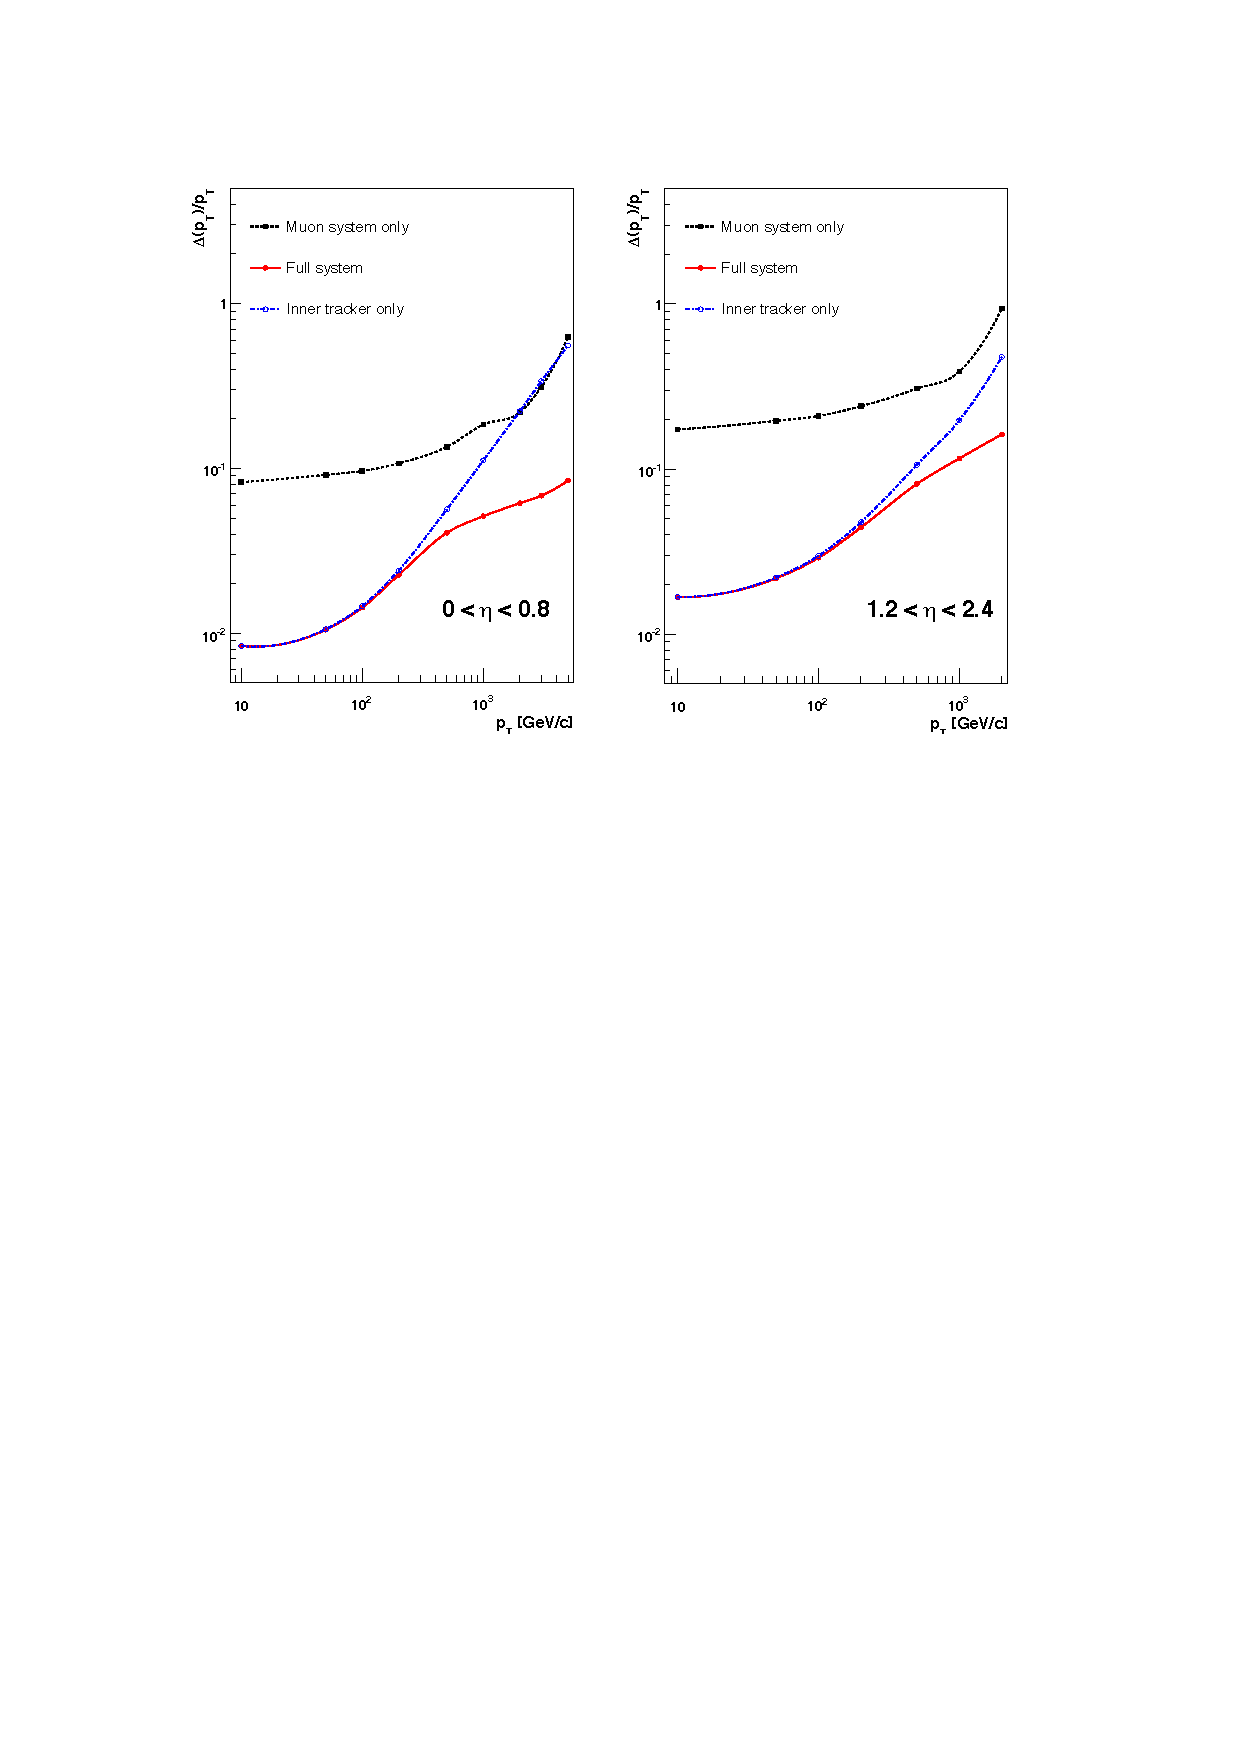
\includegraphics[scale=1.0]{muon_pT_res}
	\caption{Muon $p_{T}$ resolution as a function of muon $p_{T}$ for tracker information only (blue), muon information only (black), and both tracker and muon information combined (red).  Reprinted from Fig. 1.2 of ref. \cite{1748-0221-3-08-S08004}.}
	\label{fig:muon_pT_res}
\end{figure}

\begin{figure}
	\centering
	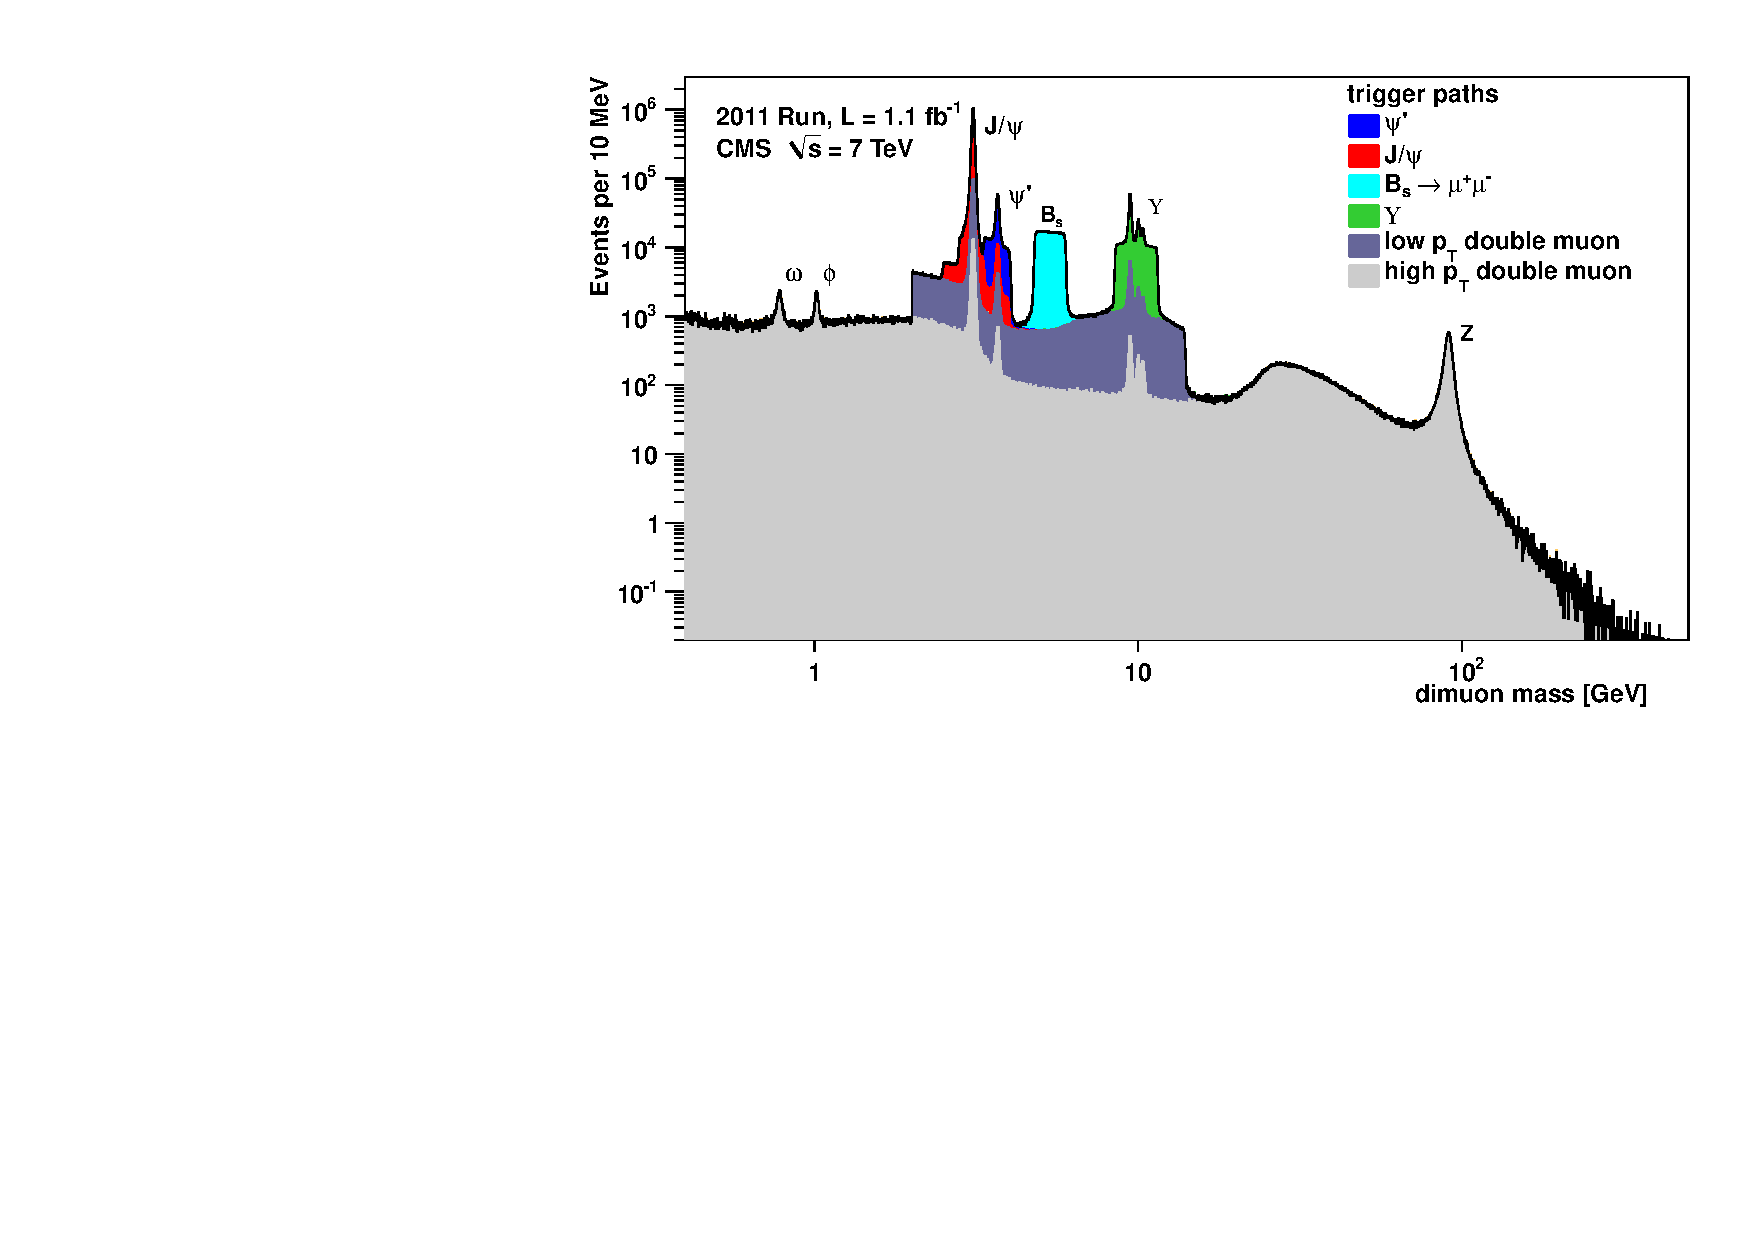
\includegraphics[scale=0.7]{muon_inv_mass}
	\caption{Di-muon invariant mass spectrum broken down by trigger path \cite{MUO_POG_Twiki_inv_mass}.  The light(dark) gray regions show the contribution from high-$p_{T}$(low-$p_{T}$) di-muon triggers.  Note that no $B_{s}\rightarrow\mu^{+}\mu^{-}$ decays have been observed \cite{springerlink:10.1007/JHEP04(2012)033}; the light blue region just shows the amount of triggers dedicated to the $B_{s}\rightarrow\mu^{+}\mu^{-}$ search.}
	\label{fig:muon_inv_mass}
\end{figure}

\section{Triggering, Data Acquisition, and Data Transfer}
\label{sec:Triggering, Data Acquisition, and Data Transfer}

\subsection{Level 1 and High Level Trigger Systems}
\label{sec:Level 1 and High Level Trigger Systems}

The Level-1 (L1) trigger system, which encompasses dedicated hardware processors to construct trigger objects (typically high $p_{T}$ jets, electrons, photons, taus, and muons) out of the calorimeter and muon hits, distributes a L1 accept or reject to all subdetectors at the LHC bunch crossing frequency of 40 MHz.  Further data filtering is performed by the High Level Trigger (HLT) system, a farm of $\sim1000$ commercially available processors running a slimmed down version of the CMS event reconstruction software CMSSW.  The data rate received by the HLT is $\sim100$ kHz; the output rate of events permanently written to disk is $\sim100$ Hz.  An L1 trigger \textit{latency} (time between the collision and the distribution of the L1 decision to the subdetectors) of 3.2 $\mu\mbox{s}$ is achieved via the use of fast electronics and sufficiently deep buffers to pipeline trigger primitives waiting to be analyzed.  This latency corresponds to the length of the LHC abort gap, so in principle CMS may be operated with zero \textit{dead time} (during which LHC bunches are missed because the L1 system is blocked while processing other triggers).

At the bottom, the L1 trigger consists of trigger primitive generators (TPGs) in the calorimeter and muon systems that send $E_{T}$ sums or muon track stubs to the regional calorimeter trigger (RCT) or muon track finders, respectively.  The EB TPG also sends a \textit{fine grain veto bit} \cite{1546528}, which encodes information about the EM shower pattern in the $5\times5$ array of crystals, and is used to reject anomalous signals (see Sec.~\ref{sec:Calibrated EB/EE Hits}).  The RCT, DT track finder (DTTF), and CSC track finder (CSCTF) sort and rank the regional trigger primitives based on $p_{T}$ and quality.  The ranked RCT candidates and muon track stubs are sent to the global calorimeter trigger (GMT) and global muon trigger (GMT), respectively, where high-level objects like isolated and non-isolated muons and EM candidates, jets, taus, and \MET are constructed from all the regional inputs and ranked.  Calorimeter isolation sums for muons are also sent from the RCT to the GMT.  The highest ranked global objects are sent to the global trigger (GT), which sits at the top of the L1 trigger.  The GT issues the final L1 accept or reject to all subdetectors based on a comparison of the GMT and GCT candidates with the requirements of its programmed trigger menu.  A block diagram of the L1 trigger is shown in Figure~\ref{fig:L1_trigger_diagram}.

\begin{figure}
	\centering
	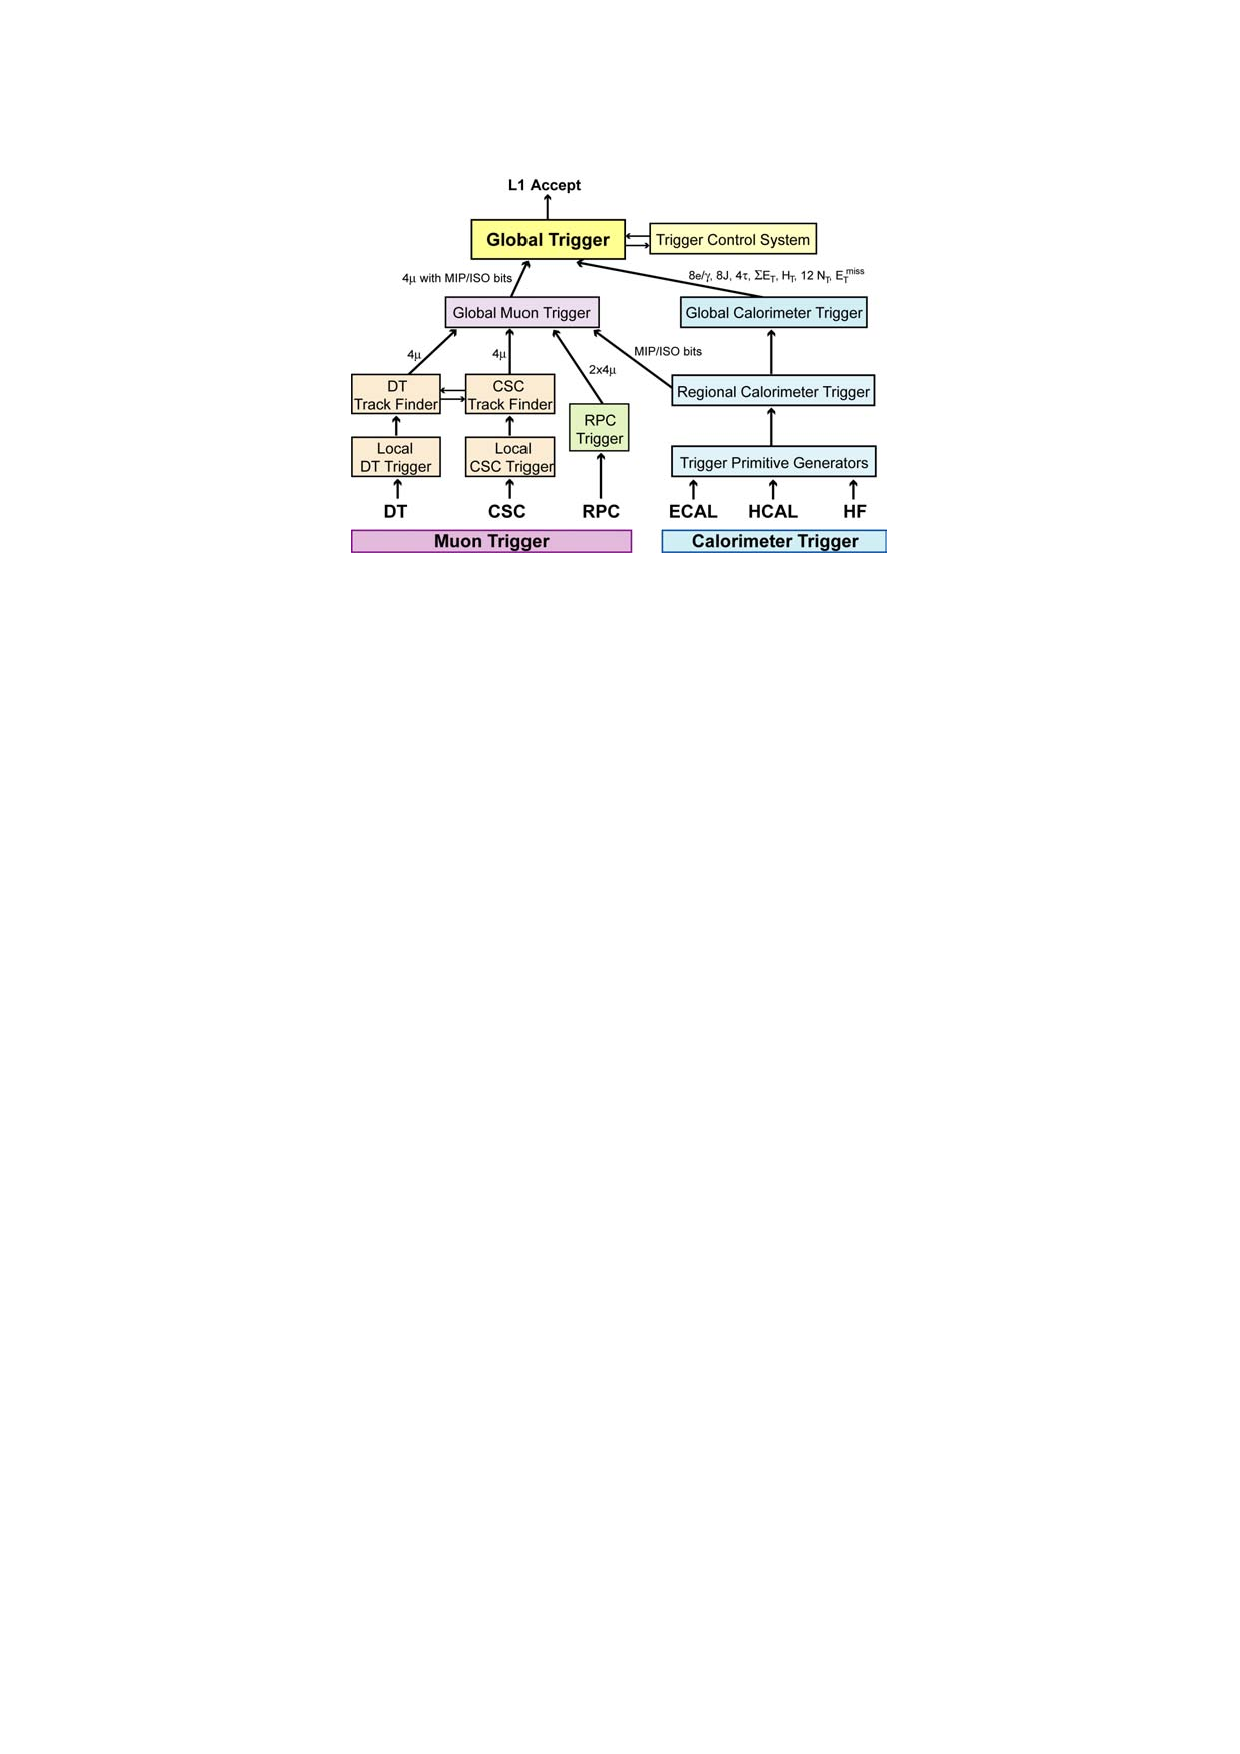
\includegraphics[scale=1.0]{L1_trigger_diagram}
	\caption{Block diagram of the L1 trigger.  Reprinted from Fig. 8.1 of ref. \cite{1748-0221-3-08-S08004}.}
	\label{fig:L1_trigger_diagram}
\end{figure}

A region in the RCT consists of a matrix of $4\times4$ trigger towers.  A trigger tower in EB/HB is one HCAL tower + the $5\times5$ matrix of ECAL crystals in front of it; in EE/HE the idea is similar but the counting of crystals and HE towers is slightly more complicated.  An EM RCT candidate is built around a high $E_{T}$ seed tower.  The $E_{T}$ of the candidate is the sum of the tower $E_{T}$ and the $E_{T}$ of its highest-$E_{T}$ broad side neighbor (see Figure~\ref{fig:RCT_EG_candidate} for a definition of the broad side neighbors).  Two isolation criteria are defined based on (a) the ratio of the EM energy to the HCAL energy in the tower and (b) the shower shape.  For a non-isolated EM candidate, the highest-$E_{T}$ broad side neighboring tower must pass these two isolation criteria; for an isolated EM candidate, all eight neighboring towers must the criteria, and there must also be at least one quiet corner with the $E_{T}$ of all five towers in the corner below some threshold (see Fig.~\ref{fig:RCT_EG_candidate}).  The process is repeated until four isolated and four non-isolated EM candidates are found, starting with the highest-$E_{T}$ tower in the region and moving down in tower $E_{T}$.  An RCT region is flagged as consistent with tau decay only if the pattern of tower transverse energy sums defines at most a $2\times2$ matrix of energetic towers within the $4\times4$ RCT region.

\begin{figure}
	\centering
	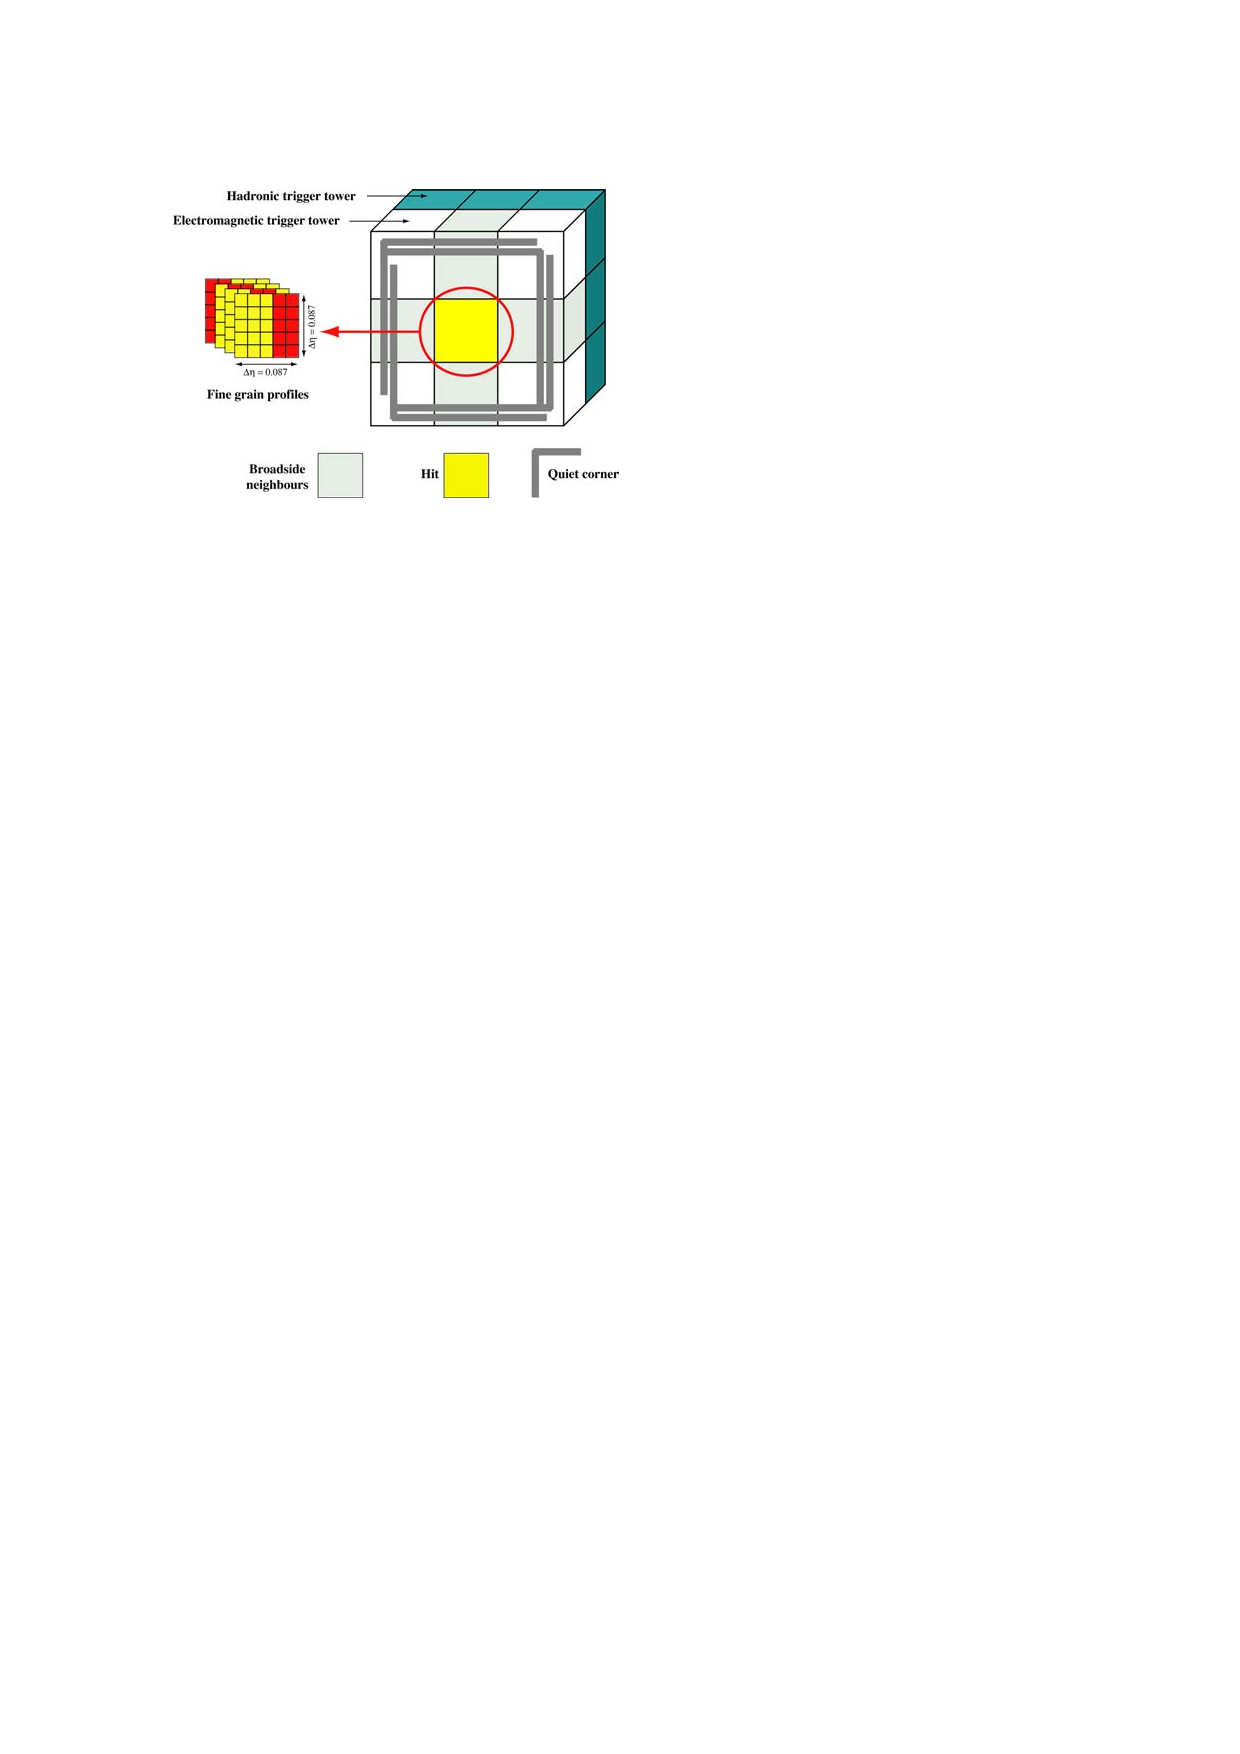
\includegraphics[scale=1.0]{RCT_EG_candidate}
	\caption{Geometry of an EM RCT candidate.  Reprinted from Fig. 8.2 of ref. \cite{1748-0221-3-08-S08004}.}
	\label{fig:RCT_EG_candidate}
\end{figure}

From the tower transverse energy sums, eight EM candidates, and tau flag received from each RCT, the GCT computes the total $E_{T}$ in the calorimeter (and the total $E_{T}$ above some programmable threshold, called $H_{T}$), and the \MET.  It also classifies the towers into jets and determines the globally highest ranked isolated and non-isolated EM candidates.  The jet finding uses a clustering algorithm based on the energy of a sub-cluster with respect to its neighbors \cite{Smith}.  Jets are classified as tau decays if all of the RCT regions participating in the jet clustering had energy patterns consistent with tau decay.  Counts of jets above 12 different programmable $E_{T}$ thresholds are calculated.  The jet counts, energy sums, \MET, and highest ranked EM candidates are sent to the GT, where the final L1 decision is taken and transmitted to the sub-detectors.  The GT can execute a maximum of 128 trigger algorithms in parallel.  If any one of these algorithms yields an accept, the event is accepted, and all trigger information is sent on to the HLT for further filtering.  The double-photon HLT paths used in this analysis (see Sec.~\ref{sec:HLT}) require isolated L1 seeds (i.e. EM candidates built by the RCT) with $E_{T} > 12$ or 20 GeV, depending on path.

No muon triggers are used in the two-photon analysis.  A description of the muon trigger system can be found in ref.\cite{1748-0221-3-08-S08004}.

\subsection{Data Acquisition System}
\label{sec:Data Acquisition System}

The CMS data acquisition (DAQ) system takes event fragments (calorimeter hits, track hits, etc.) from each of the 626 subdetector front end drivers (FEDs), assembles them into a data structure representing the full event, and sends the event on to the HLT for further filtering.  The DAQ must operate at an input rate of $\sim100$ GB/s, corresponding to an input rate from the L1 trigger of $\sim100$ kHz.  To facilitate expansion of the system as the need arises, the DAQ is composed of eight nearly independent slices.  Each slice functions as a smaller version of the whole DAQ that can handle an input event rate up to $\sim12.5$ kHz.  A diagram of the DAQ system, showing schematically the eight slices, is given in Figure~\ref{fig:DAQ_overview}.

\begin{figure}
	\centering
	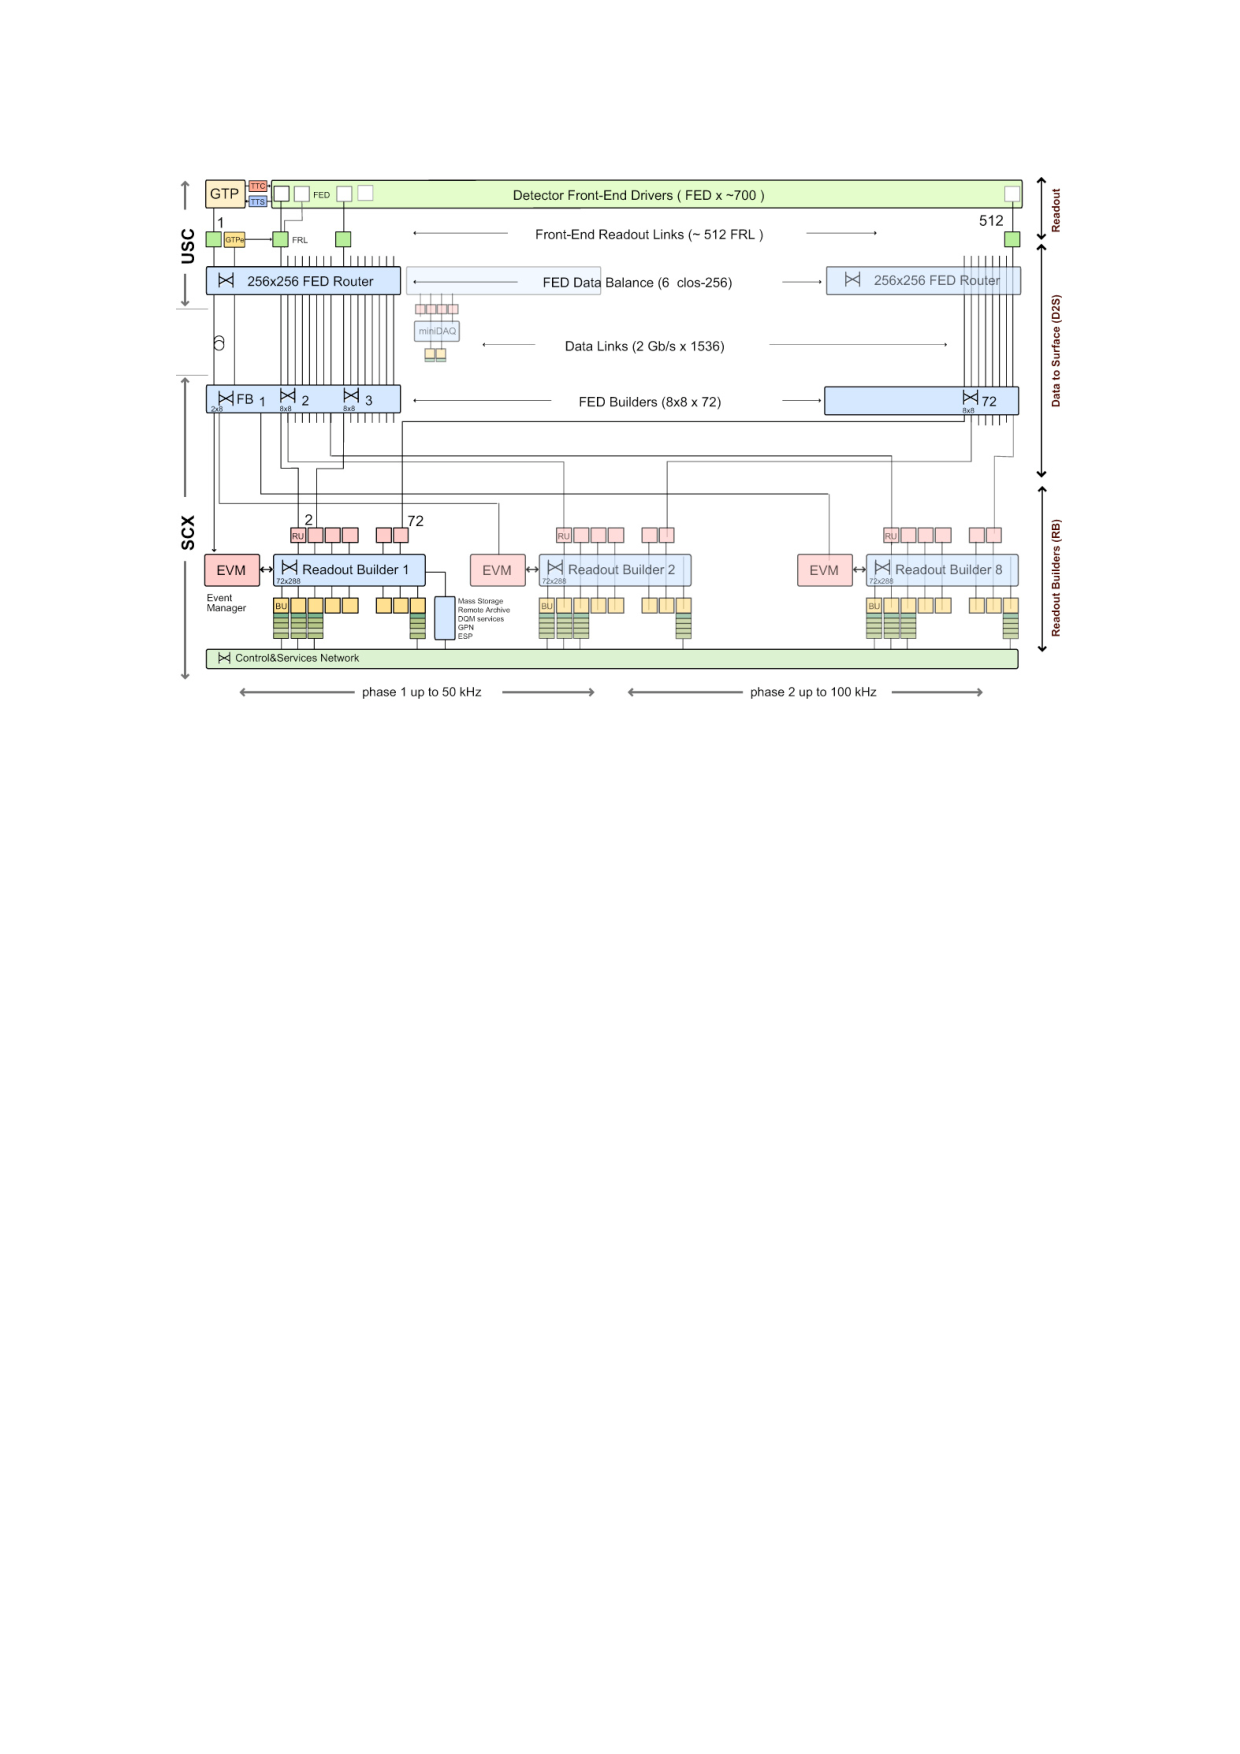
\includegraphics[scale=1.0]{DAQ_overview}
	\caption{Diagram of the DAQ system.  The identical event builder systems, shown as inputs and outputs to the boxes labeled ``Readout Builder 1", ``Readout Builder 2", etc., represent the eight slices.  Within one slice, data can flow from the detector front ends to the readout systems to the builder network (which assembles the event fragments) to the filter systems (HLT) independently of the other slices.  Reprinted from Fig. 9.8 of ref. \cite{1748-0221-3-08-S08004}.}
	\label{fig:DAQ_overview}
\end{figure}

Data from the front ends is collected by the FEDs and pushed to the front end readout links (FRLs), which may take inputs from up to two FEDs simultaneously.  The FRLs check for transmission errors, generate event fragments with size $\sim2$ kB, buffer the fragments in 64 kB memories, and finally send them to the FED builders.  The FEDs, FRLs, and FED builders are located in the underground control room.  The 72 FED builders each construct one $\sim16$ kB \textit{super-fragment} from the input event fragments, then send the super-fragment on to a readout unit (RU) located in the surface control room $\sim80$ m away.  Super-fragments belonging to the same event are sent to RUs in the same DAQ slice.  There are 72 RUs per readout builder, one for each super-fragment of an event, with each DAQ slice built around one readout builder (see Fig.~\ref{fig:DAQ_overview}).  Each readout builder hosts a number of builder units (BUs) that perform the final integration of super-fragments into complete events.

Resource brokers (RBs) in the HLT filter farm request complete events from the BUs and distribute those events to the filter units (FUs) for HLT selection.  If an event passes any one of the HLT paths in the predefined menu, it is sent back to the RB for transfer to the storage manager (SM).  The SM nodes transfer accepted events to the CERN Tier-0 prompt reconstruction facility for unpacking of the raw data into ROOT \cite{Brun199781} files that can be accessed by physicists wishing analyze the data.  The lag time between recording of an event in the DAQ and availability of the fully reconstructed event for analysis is typically 48 hours.

If the buffers of the upstream DAQ elements (the filter farm, readout builders, FED builders, or FRLs) are full, those elements will not request new events from downstream.  This can lead to a buildup of events in the downstream element buffers, \textit{back-pressuring} all the way down to the FEDs themselves.  The CMS trigger throttling system (TTS) consists of dedicated lines between the FEDs and the GT for the purpose of sending predefined signals to the GT about the state of the FED buffers.  If the buffer of a particular FED is getting full, it can alert the GT to reduce the trigger rate so as to prevent FED buffer overflows and loss of time synchronization between event fragments.  The TTS latency is $\sim1 \mu\mbox{s}$.  Causes of back-pressure (hence dead time) include: problems with the FED electronics (in this case, the upstream elements request events but the FEDs have trouble sending them), increases in the L1 accept rate (perhaps due to a noisy detector channel) beyond what the upstream DAQ elements can handle, increases in the event size due to high pileup or a poor quality beam that scrapes against the beam pipe, failures of the DAQ transmission lines or DAQ hardware such that events are not requested from the FEDs fast enough, or bottlenecks at the SM nodes or filter farm due to hardware failures or large event sizes.

All components of the DAQ, from the FEDs up to the SMs, are controlled by cross-platform DAQ (XDAQ) \cite{springerlink:10.1023/A:1012744721976} processes, or \textit{executives}.  The Simple Object Access Protocol (SOAP) \cite{SOAP} protocol is used to transmit control and monitoring data between XDAQ-enabled devices and to the end user, who can view the running of a XDAQ executive via a Web interface called HyperDAQ \cite{HyperDAQ}.  The Run Control and Monitoring System (RCMS) handles the configuration and control of all XDAQ executives via a hierarchical structure.  At the top of the hierarchy is the Level-0 \textit{function manager} (FM), controlling the Level-1 sub-detector FMs, which in turn control their Level-2 system-specific XDAQ executives.  The central DAQ and L1 trigger each have their own Level-1 FM.  A unit of data acquisition, called a \textit{run}, may be configured, started, and stopped by an end user interacting with the RCMS Web interface.

\subsection{Data Processing and Transfer to Computing Centers}
\label{sec:Data Processing and Transfer to Computing Centers}

Data leaving the filter farm are grouped into datasets based on HLT path, i.e. there are different datasets for events passing diphoton triggers, jet triggers, muon + electron triggers, etc.  At the Tier-0 facility, the datasets are go through three levels of processing to create three \textit{data tiers}.  The first layer produces RAW data by unpacking the detector byte streams sent from the DAQ and L1 trigger into data structures holding the ADC counts recorded for each channel of the detector, digitized trigger primitives, and the L1 decision.  A single event has $\sim1.5$ MB of RAW data.  The next layer of processing is the reconstruction, which forms channel energies in GeV, applies calibrations, and creates high-level objects like photons, electrons, muons, taus, jets, \MET, and charged tracks.  The RECO data tier occupies $\sim0.5$ MB per event.  Finally, analysis object data (AOD) is a subset of the RECO data, comprising the high-level objects but usually excluding the individual channel hit information if it is not associated to a physics object.  This tier occupies $\sim0.1$ MB per event.  One copy of the RAW data is stored permanently at CERN and another copy is distributed amongst the Tier-1 facilities (see below) for permanent storage.  Changes in the reconstruction algorithms periodically require reprocessing of the RAW data to form a new RECO tier.  In general, only the AOD tier is available to physicists wishing to perform analyses due to the smaller size and faster replication and transfer time of AOD with respect to RAW or RECO.

There are three tiers of computing and data storage sites within the Worldwide LHC Computing Grid (WLCG) \cite{Eck:840543}.  The tier closest to CMS is Tier-0, which is located at CERN and performs archiving of the RAW data, prompt reconstruction of the data within $\sim48$ hours of its being collected, and transferral of copies of the RECO datasets to Tier-1 facilities.  There are a few Tier-1 centers worldwide, hosted by national computing facilities and laboratories.  They store parts of the RAW dataset and copies of the RECO datasets, participate in subsequent reconstruction passes after the prompt reconstruction at Tier-0, and ship AOD datasets upon request to the Tier-2 centers.  Analysts interact primarily with the Tier-2 centers, which store AOD datasets and run batch processing queues for running analysis jobs over the datasets.  Different layers of WLCG software control data transfer between sites, data storage, and batch processing.  A diagram of the WLCG tier system is given in Figure~\ref{fig:WLCG_diagram}.

\begin{figure}
	\centering
	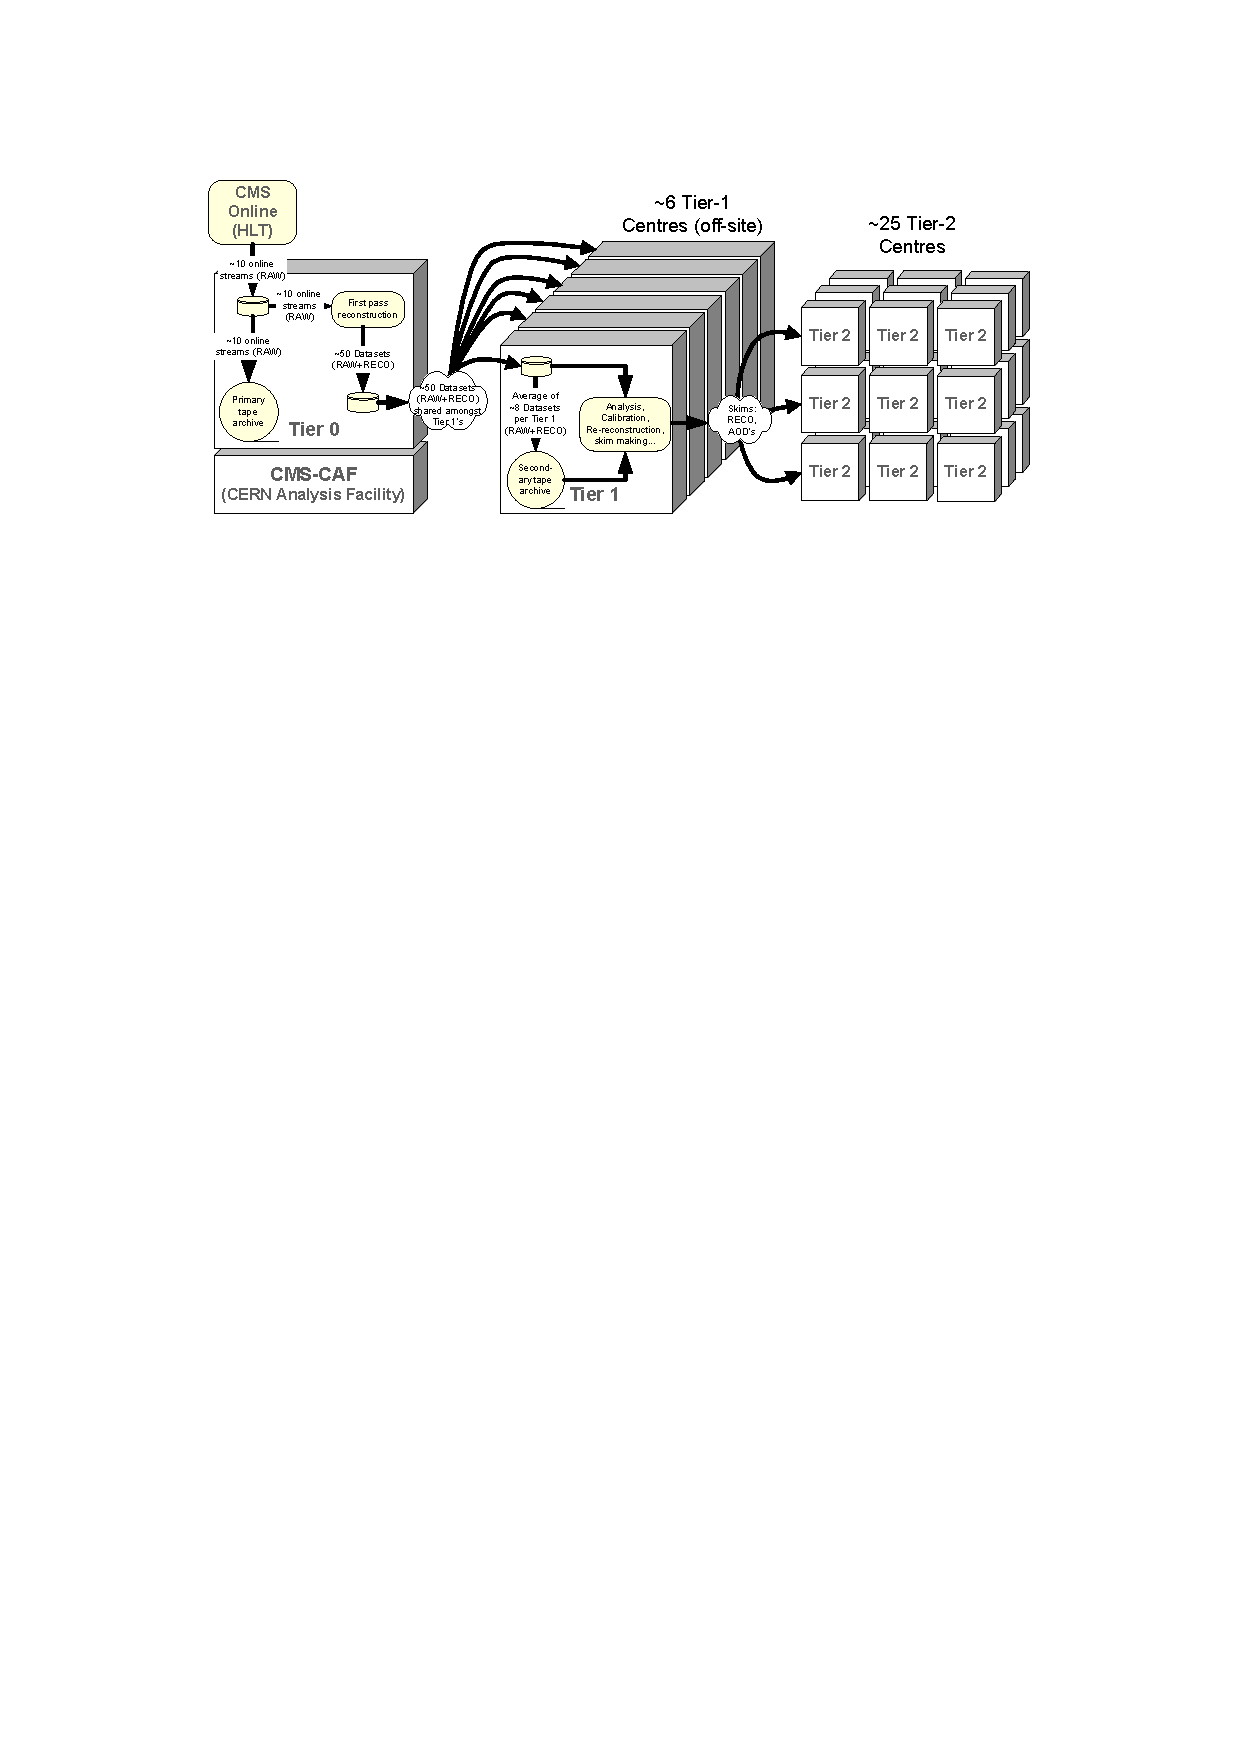
\includegraphics[scale=1.0]{WLCG_diagram}
	\caption{Diagram of the WLCG tier system showing data archival and reconstruction at each tier along with data transfer between tiers.  Reprinted from Fig. 11.2 of ref. \cite{1748-0221-3-08-S08004}.}
	\label{fig:WLCG_diagram}
\end{figure}

\end{document}